% ============================================================
% CO3043 - Phát triển Ứng dụng trên Thiết bị Di động (HCMUT)
% OneSpace — Ứng dụng giải trí tích hợp 4-trong-1 trên Android
% Presentation - team: Pham Khanh Duy, Nguyen Tran Yen Nhi, Tang Hong Ai
% Style: mirrors the DataWarehouse midterm deck (Madrid + BKTemplate)
% Structure: 4 sections — Giới thiệu · Phạm vi sản phẩm · UI/UX · Kiến trúc kỹ thuật
% ============================================================
\documentclass[aspectratio=169]{beamer}
\usetheme{Madrid}
\usefonttheme{structurebold}
\usefonttheme[onlymath]{serif}

\definecolor{BKTemplate}{rgb}{0.11765, 0.30588, 0.47451}
\usecolortheme[named=BKTemplate]{structure}
\setbeamercolor{title}{fg=BKTemplate,bg=}
\usepackage{xcolor}
\setbeamertemplate{caption}[numbered]
\setbeamertemplate{navigation symbols}{}
\usepackage[utf8]{inputenc}
\usepackage[T1]{fontenc}
\usepackage[utf8]{vntex}   % Vietnamese diacritics (T5 encoding), as in the team report
\usepackage[english]{babel}
\usepackage{lmodern}       % vector Type 1 fonts for T1 + T5: no bitmap glyphs
\usepackage{url}
\usepackage{booktabs}
\usepackage{amsfonts}
\usepackage{amsmath}
\usepackage{amssymb}
\usepackage{array}
\usepackage{multirow}
\usepackage{multicol}
\usepackage{graphicx}
\usepackage{colortbl}
\usepackage{tikz}
\usetikzlibrary{positioning, arrows.meta, shapes.geometric, calc, fit}
\usepackage{hyperref}
\renewcommand\UrlFont{\color{blue}\rmfamily}

% Custom colors
\definecolor{AccentGold}{HTML}{E8A838}
\definecolor{BKDark}{HTML}{0D2B45}
\definecolor{BKLight}{HTML}{2A6BA5}
\definecolor{LightBG}{HTML}{F0F4F8}
\definecolor{TextGray}{HTML}{5A6C7D}
\definecolor{GreenOK}{HTML}{27AE60}
\definecolor{RedNo}{HTML}{E74C3C}
\definecolor{OrangeWarn}{HTML}{F39C12}

%------------------------------------------------------------
% Ký hiệu ma trận đối thủ
%------------------------------------------------------------
\newcommand{\cmark}{\textcolor{GreenOK}{\checkmark}}
\newcommand{\pmark}{\textcolor{OrangeWarn}{$\triangle$}}
\newcommand{\xmark}{\textcolor{TextGray}{$\times$}}

%------------------------------------------------------------
% Ô màu swatch cho bảng design token
%------------------------------------------------------------
\newcommand{\sw}[2]{\colorbox[HTML]{#1}{\textcolor[HTML]{#2}{\rule[-2.5pt]{13pt}{13pt}}}}

%------------------------------------------------------------
% Ảnh mockup. Một tính năng có thể có NHIỀU ảnh chụp, đánh số
% liên tiếp: figures/app/<mã>-01.png, -02.png, ... (tối đa 6).
% Thư mục tìm kiếm: presentation/figures/app rồi figures/app của
% repo; chưa có ảnh nào thì vẽ khung placeholder.
% \imgdir  — tiền tố thư mục chứa ảnh (rỗng hoặc ../)
% \imgn    — số ảnh tìm thấy (đánh số liền kề từ 01)
%------------------------------------------------------------
\newcommand{\mockimg}[1]{%
  \def\imgdir{}%
  \IfFileExists{figures/app/#1-01.png}{}{%
    \IfFileExists{../figures/app/#1-01.png}{\def\imgdir{../}}{}%
  }%
  \def\imgn{0}%
  \IfFileExists{\imgdir figures/app/#1-01.png}{\def\imgn{1}}{}%
  \ifnum\imgn>0 \IfFileExists{\imgdir figures/app/#1-02.png}{\def\imgn{2}}{}\fi
  \ifnum\imgn>1 \IfFileExists{\imgdir figures/app/#1-03.png}{\def\imgn{3}}{}\fi
  \ifnum\imgn>2 \IfFileExists{\imgdir figures/app/#1-04.png}{\def\imgn{4}}{}\fi
  \ifnum\imgn>3 \IfFileExists{\imgdir figures/app/#1-05.png}{\def\imgn{5}}{}\fi
  \ifnum\imgn>4 \IfFileExists{\imgdir figures/app/#1-06.png}{\def\imgn{6}}{}\fi
  \ifnum\imgn=0
    % Kiểu cũ: đúng một tệp <mã>.png
    \IfFileExists{figures/app/#1.png}{%
      \includegraphics[height=6.1cm]{figures/app/#1.png}%
    }{%
    \IfFileExists{../figures/app/#1.png}{%
      \includegraphics[height=6.1cm]{../figures/app/#1.png}%
    }{%
      \begin{tikzpicture}
        \node[draw=BKTemplate!60, dashed, thick, rounded corners=6pt, fill=LightBG,
              minimum width=3.1cm, minimum height=5.2cm, align=center] {%
          {\small\bfseries\color{BKTemplate} Mockup}\\[3pt]
          {\scriptsize\ttfamily\color{TextGray} \imgdir figures/app/#1-01.png}};
      \end{tikzpicture}%
    }}%
  \else
    \ifcase\imgn
    \or % 1 ảnh
      \includegraphics[height=6.1cm]{\imgdir figures/app/#1-01.png}%
    \or % 2 ảnh
      \includegraphics[width=2.75cm]{\imgdir figures/app/#1-01.png}\hspace{0.25cm}%
      \includegraphics[width=2.75cm]{\imgdir figures/app/#1-02.png}%
    \or % 3 ảnh
      \includegraphics[width=2.32cm]{\imgdir figures/app/#1-01.png}\hspace{0.2cm}%
      \includegraphics[width=2.32cm]{\imgdir figures/app/#1-02.png}\hspace{0.2cm}%
      \includegraphics[width=2.32cm]{\imgdir figures/app/#1-03.png}%
    \or % 4 ảnh
      \includegraphics[width=1.72cm]{\imgdir figures/app/#1-01.png}\hspace{0.12cm}%
      \includegraphics[width=1.72cm]{\imgdir figures/app/#1-02.png}\hspace{0.12cm}%
      \includegraphics[width=1.72cm]{\imgdir figures/app/#1-03.png}\hspace{0.12cm}%
      \includegraphics[width=1.72cm]{\imgdir figures/app/#1-04.png}%
    \or % 5 ảnh
      \includegraphics[width=1.36cm]{\imgdir figures/app/#1-01.png}\hspace{0.1cm}%
      \includegraphics[width=1.36cm]{\imgdir figures/app/#1-02.png}\hspace{0.1cm}%
      \includegraphics[width=1.36cm]{\imgdir figures/app/#1-03.png}\hspace{0.1cm}%
      \includegraphics[width=1.36cm]{\imgdir figures/app/#1-04.png}\hspace{0.1cm}%
      \includegraphics[width=1.36cm]{\imgdir figures/app/#1-05.png}%
    \or % 6 ảnh
      \includegraphics[width=1.12cm]{\imgdir figures/app/#1-01.png}\hspace{0.08cm}%
      \includegraphics[width=1.12cm]{\imgdir figures/app/#1-02.png}\hspace{0.08cm}%
      \includegraphics[width=1.12cm]{\imgdir figures/app/#1-03.png}\hspace{0.08cm}%
      \includegraphics[width=1.12cm]{\imgdir figures/app/#1-04.png}\hspace{0.08cm}%
      \includegraphics[width=1.12cm]{\imgdir figures/app/#1-05.png}\hspace{0.08cm}%
      \includegraphics[width=1.12cm]{\imgdir figures/app/#1-06.png}%
    \fi
  \fi
}

%------------------------------------------------------------
% Bố cục slide mockup: cột trái là mã + mô tả, cột phải là ảnh
% \mockbody{F-VID-01}{Tên tính năng}{mô tả}
%------------------------------------------------------------
\newcommand{\mockbody}[3]{%
\begin{columns}[T]
\begin{column}{0.46\textwidth}
{\small\bfseries\color{BKTemplate} #1: #2}\\[2.5mm]
#3
\end{column}
\begin{column}{0.50\textwidth}
\centering
\mockimg{#1}
\end{column}
\end{columns}}

%------------------------------------------------------------
% Reusable statistic card
%------------------------------------------------------------
\newcommand{\statcard}[3]{%
\begin{tikzpicture}
\node[draw=BKTemplate, line width=1pt, fill=LightBG, rounded corners=6pt,
      minimum width=2.9cm, minimum height=2.55cm, align=center, inner sep=5pt] {%
{\fontsize{32}{34}\selectfont\bfseries\color{BKTemplate}#1}\\[2pt]
{\small\bfseries\color{BKDark}#2}\\[1pt]
{\scriptsize\color{TextGray}#3}};
\end{tikzpicture}}

%------------------------------------------------------------
\title[Phát triển Ứng dụng trên Thiết bị Di động]{OneSpace --- Ứng dụng giải trí tích hợp 4-trong-1 trên Android}

\subtitle{CO3043 --- Phát triển Ứng dụng trên Thiết bị Di động · Bài tập lớn}

\author[Khoa Khoa học và Kỹ thuật Máy tính]{Phạm Khánh Duy (2310510) \and Nguyễn Trần Yến Nhi (2312506) \and Tăng Hồng Ái (2310167)}

\institute[]{Faculty of Computer Science and Engineering, HCMUT, VNU-HCM, Vietnam \and Advisor: TS.\ Phan Trần Minh Khuê}

\date[CO3043 · Nov 2026]{November 2026}

%------------------------------------------------------------
% Section divider: TOC với section hiện tại highlight, các section khác mờ
%------------------------------------------------------------
\AtBeginSection[]
{
  \begin{frame}
    \frametitle{Nội dung}
    \tableofcontents[currentsection,hideallsubsections]
  \end{frame}
}
%------------------------------------------------------------

\begin{document}

% ============================================================
% TITLE SLIDE — nền riêng FrontBackground (logo ở trên và dưới,
% khối chữ nằm giữa, chừa trống hai đầu)
% ============================================================
\setbeamertemplate{background canvas}{
    
\includegraphics[width=\paperwidth,height=\paperheight]{images/FrontBackground.pptx.pdf}
}
\begin{frame}[plain]
% Logo nền chiếm khoảng 40pt trên đỉnh; khối chữ hạ xuống dưới nó,
% mép dưới giữ nguyên (logo đáy bắt đầu ~234pt trên trang cao 255pt).
\vspace*{1.6cm}
\begin{center}
{\small\color{BKDark} Bài tập lớn môn học:}\\[1.2mm]
{\normalsize\bfseries\color{BKTemplate} Phát triển Ứng dụng trên Thiết bị Di động (CO3043)}\\[4mm]

{\small\color{BKDark} Chủ đề}\\[1.5mm]
{\Large\bfseries\color{BKTemplate} Ứng dụng giải trí đa phương tiện tích hợp}\\[1.2mm]
{\Large\bfseries\color{BKTemplate} Video, Music, News và Games}\\[4mm]

{\normalsize GVHD: TS.\ Phan Trần Minh Khuê}\\[4mm]

{\normalsize
\begin{tabular}{@{}l@{\hspace{2.5em}}l@{}}
Phạm Khánh Duy & 2310510\\[1mm]
Nguyễn Trần Yến Nhi & 2312506\\[1mm]
Tăng Hồng Ái & 2310167\\
\end{tabular}}
\end{center}
\vfill
\end{frame}

% Set background for all subsequent slides
\setbeamertemplate{background canvas}{
	
\includegraphics[width=\paperwidth,height=\paperheight]{images/Background.pdf}
}

% ============================================================
% OUTLINE
% ============================================================
\begin{frame}{Nội dung}
\begin{enumerate}
    \item \textbf{Giới thiệu} \hfill \textit{Bối cảnh thị trường, vấn đề, persona, đối thủ, SWOT, USP}
    \item \textbf{Phạm vi sản phẩm} \hfill \textit{Tiêu chí chất lượng, 76 tính năng, ma trận chuyển, user stories}
    \item \textbf{UI/UX thiết kế} \hfill \textit{Kiến trúc thông tin, luồng, mockup, design system, accessibility}
    \item \textbf{Kiến trúc kỹ thuật} \hfill \textit{Tech stack, ba lớp, mô-đun, điều hướng, dữ liệu, TTS}
\end{enumerate}
\end{frame}

% ============================================================
% CONTENT
% ============================================================
% ============================================================
% SECTION 1 - GIỚI THIỆU
% Bối cảnh → Phát biểu bài toán → Phân loại → Thị trường
% → Đối thủ → SWOT → Personas → USP & Winning Zone
% ============================================================
\section{Giới thiệu}

% ------------------------------------------------------------
% Slide giới thiệu app: logo + tên + mô tả tổng quan
% ------------------------------------------------------------
\begin{frame}
\vfill
\begin{center}
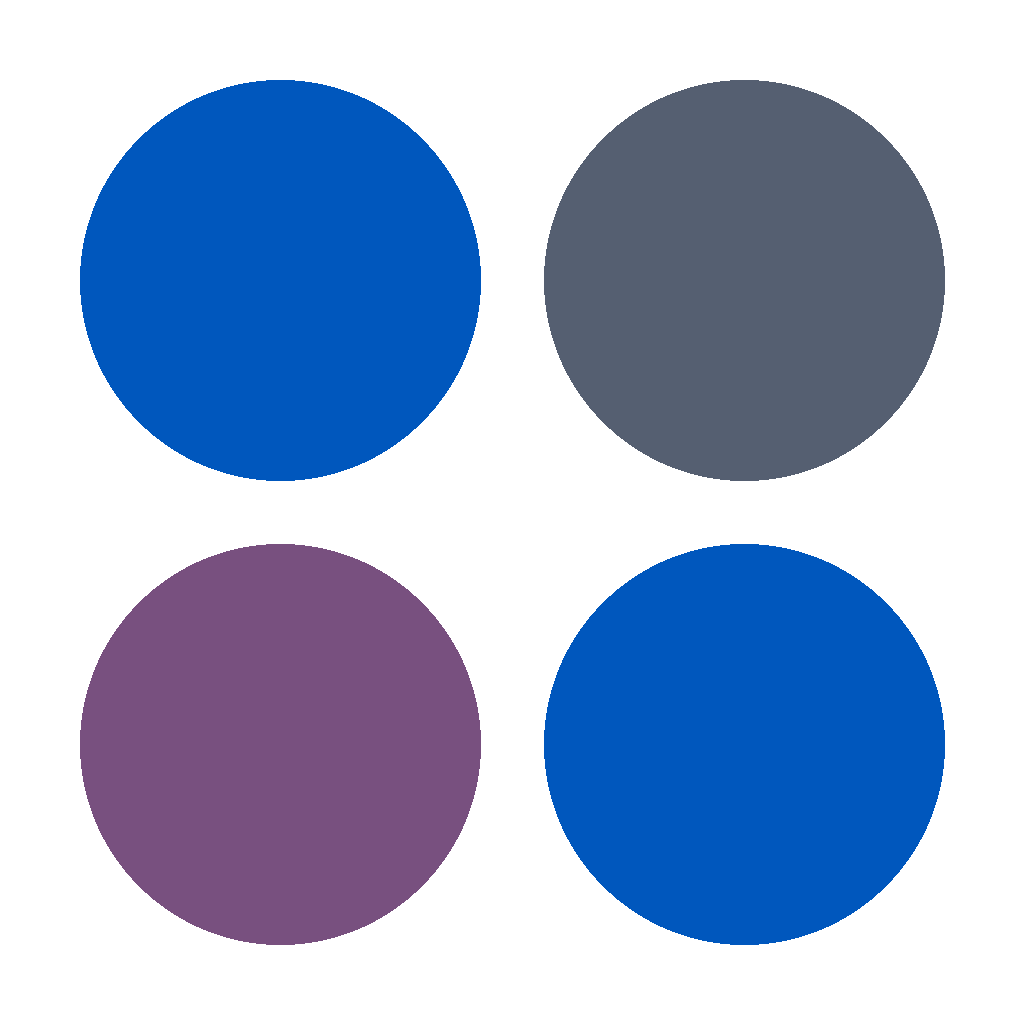
\includegraphics[height=2.9cm]{figures/onespace-logo-transparent.png}\\[2.5mm]
{\LARGE\bfseries\color{BKTemplate} OneSpace}\\[1.5mm]
{\small\bfseries\color{BKDark} Ứng dụng giải trí tích hợp 4-trong-1 trên Android}\\[4mm]
\begin{minipage}{0.86\textwidth}
\begin{exampleblock}{Mô tả tổng quan}
{\small Một ứng dụng duy nhất cho bốn nhu cầu giải trí: xem video, nghe nhạc, đọc tin và chơi minigame. Nội dung đi theo người dùng khi đổi hoạt động~--~nhạc chạy nền, video nổi, bài đọc thu thành thẻ~--~nên trải nghiệm liền mạch thay vì bốn ứng dụng rời rạc.}
\end{exampleblock}
\end{minipage}
\end{center}
\vfill
\end{frame}

% ------------------------------------------------------------
\subsection{Bối cảnh}
% ------------------------------------------------------------
\begin{frame}{Bối cảnh}
\begin{columns}[T]
\begin{column}{0.52\textwidth}
\footnotesize
\begin{itemize}\setlength{\itemsep}{3pt}
\item Điện thoại là thiết bị giải trí chính của người Việt:
      \textbf{137 triệu} kết nối di động (134\% dân số);
      \textbf{85,6 triệu} người dùng Internet (84,2\%)
\item 82\% người được khảo sát dùng TikTok trong 7 ngày gần nhất;
      dành \textbf{7,1 giờ/ngày} cho ứng dụng di động và dùng hơn \textbf{27 ứng dụng/tuần}
\item Mỗi loại nội dung một bộ ứng dụng riêng:
      Video (YouTube, TikTok\ldots), Âm nhạc (Spotify, Zing\ldots),
      Tin tức (VnExpress, Báo Mới\ldots), Minigame: rời rạc trên Facebook, YouTube Playables, Shopee\ldots
\end{itemize}
\end{column}
\begin{column}{0.44\textwidth}
\centering
\vspace{1mm}

\includegraphics[height=1.9cm,keepaspectratio=true]{figures/Bối cảnh-01.png}\\[3pt]

\includegraphics[height=1.9cm,keepaspectratio=true]{figures/Bối cảnh-02.png}\\[3pt]
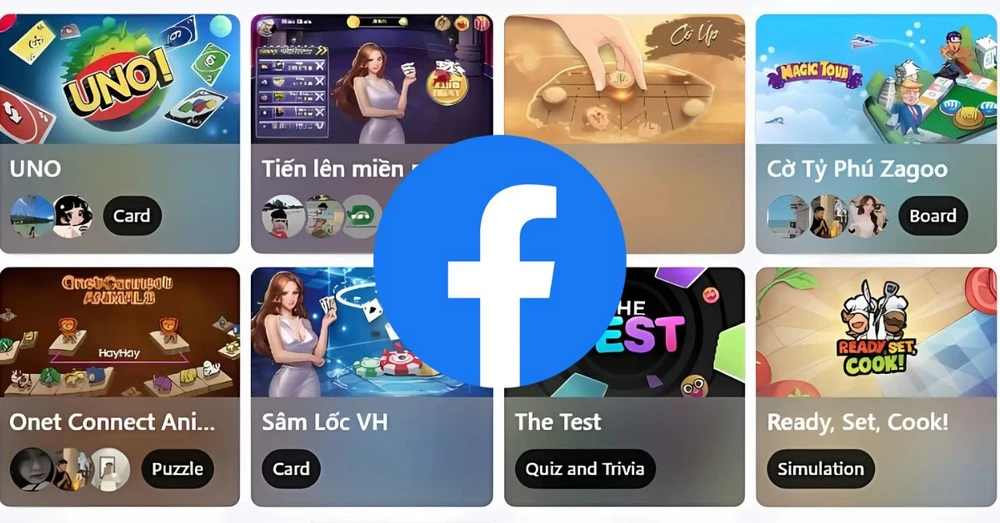
\includegraphics[height=1.9cm,keepaspectratio=true]{figures/Bối cảnh-03.png}
\end{column}
\end{columns}
\end{frame}

% ------------------------------------------------------------
\subsection{Phát biểu bài toán}
% ------------------------------------------------------------
\begin{frame}{Phát biểu bài toán}
\begin{columns}[T]
\begin{column}{0.54\textwidth}
\footnotesize
\begin{block}{Trải nghiệm đứt gãy (Context Switching)}
\begin{itemize}\setlength{\itemsep}{1pt}
\item Nội dung không theo người dùng khi đổi ngữ cảnh
\item Chế độ thu nhỏ picture-in-picture (PIP) tuỳ app
\item Khó phối hợp âm thanh
\end{itemize}
\end{block}
\vspace{-0.06cm}
\begin{block}{Tài khoản \& thông báo}
Đăng nhập nhiều lần, thông báo đẩy chồng chéo
\end{block}
\vspace{-0.06cm}
\begin{block}{Tài nguyên}
Nhiều ứng dụng chiếm nhiều không gian lưu trữ, RAM khi chạy nền, cạn pin
\end{block}
\end{column}
\begin{column}{0.43\textwidth}
\begin{alertblock}{Bài toán}
\small\itshape
``Làm thế nào để thiết kế một ứng dụng Android hợp nhất bốn phân hệ Streaming Video, Listening to Music, Reading News và Playing Minigames trong một trải nghiệm liền mạch, và giá trị khác biệt nào khiến người dùng chọn ứng dụng này thay vì tiếp tục dùng các ứng dụng quen thuộc hiện tại?''
\end{alertblock}
\end{column}
\end{columns}
\end{frame}

% ------------------------------------------------------------
\subsection{Phân tích bài toán và thu thập yêu cầu}
% ------------------------------------------------------------
\begin{frame}{Phân tích bài toán \& thu thập yêu cầu}
\begin{columns}[T]
\begin{column}{0.31\textwidth}
\begin{block}{\scriptsize\bfseries Nghiên cứu thị trường}
{\tiny
\begin{itemize}\setlength{\itemsep}{1.5pt}
\item DataReportal Digital 2026: 85,6~triệu người dùng Internet (84,2\%)
\item StatCounter 9/2026: Android 59,77\% thị phần di động
\item Q\&Me 2026: 7,1~giờ/ngày, 27+ app/tuần (mẫu 100 người dùng iPhone)
\end{itemize}}
\end{block}
\end{column}
\begin{column}{0.31\textwidth}
\begin{block}{\scriptsize\bfseries Phân tích app đối thủ}
{\tiny
\begin{itemize}\setlength{\itemsep}{1.5pt}
\item Dùng trực tiếp YouTube, TikTok, Mocha; đối chiếu 6 nền tảng gián tiếp
\item Ma trận tính năng 6 đối thủ $\times$ 4 dạng nội dung
\item 3.750 review App Store VN (2021--2026): pain point liền mạch lặp lại
\end{itemize}}
\end{block}
\end{column}
\begin{column}{0.31\textwidth}
\begin{block}{\scriptsize\bfseries Phân tích người dùng}
{\tiny
\begin{itemize}\setlength{\itemsep}{1.5pt}
\item 6 chân dung người dùng theo hành vi tiêu thụ nội dung
\item Pain: đứt gãy ngữ cảnh, khó phối hợp âm thanh, khó tiếp cận
\end{itemize}}
\end{block}
\end{column}
\end{columns}
\vspace{1mm}
\begin{block}{\scriptsize\bfseries Bằng chứng người dùng thật --- trích review App Store Việt Nam}
{\tiny
\begin{itemize}\setlength{\itemsep}{1pt}
\item \textbf{YouTube} (1/5$\bigstar$, 11/2026): ``\ldots không thu nhỏ video để vừa xem vừa dùng app khác, phải pause play lại mới được''
\item \textbf{Zing MP3} (2/5$\bigstar$, 10/2026): ``hay dùng để nghe nhạc khi chơi ff \ldots\ cứ ra sảnh lại mất nhạc''\quad·\quad \textbf{Zalo} (1/5$\bigstar$, 2026): ``spam liên tục \ldots\ mất tập trung''
\item \textbf{VnExpress} (1/5$\bigstar$, 2024): ``nặng tốn dung lượng, tốn pin dễ nóng máy''
\end{itemize}}
\end{block}
\vspace{0.8mm}
{\tiny\color{TextGray} Stakeholder: người dùng cuối (6 persona) $\cdot$ nhóm phát triển $\cdot$ nhà trường / GVHD $\cdot$ nền tảng (Google Play, AdMob). \quad Đầu ra: 76 tính năng $\rightarrow$ C1--C12 $\rightarrow$ 45 user story.}
\end{frame}

% ------------------------------------------------------------
\subsection{Phân loại ứng dụng}
% ------------------------------------------------------------
\begin{frame}{Phân loại ứng dụng}
\begin{columns}[T]
\begin{column}{0.52\textwidth}
\footnotesize
\begin{block}{Primary}
\textbf{Entertainment}
\end{block}
\vspace{1pt}
\begin{block}{Secondary}
\begin{itemize}\setlength{\itemsep}{1pt}
\item Music \& Audio
\item News \& Magazines
\item Video Players \& Editors
\item Games --- Casual / Puzzle / Trivia
\end{itemize}
\end{block}
\end{column}
\begin{column}{0.44\textwidth}
\centering

\includegraphics[width=0.95\linewidth]{figures/Phân loại-01.png}
\end{column}
\end{columns}
\end{frame}

% ------------------------------------------------------------
\subsection{Thị trường}
% ------------------------------------------------------------
\begin{frame}{Thị trường: Tổng quan}
\small
\begin{itemize}\setlength{\itemsep}{1pt}
\item Cả nước có đến \textbf{85,6 triệu} người dùng Internet (84,2\% dân số), cuối 2025
\item Trong năm 2025, Việt Nam ghi nhận \textbf{2,88 tỷ} lượt tải ứng dụng (top 11 thế giới)
\end{itemize}
\begin{center}
\scalebox{0.87}{\statcard{85,6tr}{Người dùng Internet}{84,2\% dân số, cuối 2025}\hspace{4pt}%
\statcard{2,88tỷ}{Lượt tải ứng dụng}{2025 --- top 11 thế giới}\hspace{4pt}%
\statcard{59,8\%}{Android}{thị phần HĐH di động, 9/2026}}
\end{center}
\begin{center}
\begin{tikzpicture}
% Tiêu đề tách khỏi thanh một khoảng nhìn rõ
\node[anchor=west, font=\scriptsize\bfseries, text=BKDark] at (0,0.95) {Thị phần HĐH di động (9/2026)};
% Một thanh liền: Android chiếm trước, iOS nối sau (tỉ lệ thật 59,77 : 40,19)
\fill[BKTemplate, rounded corners=3pt] (0,0.05) rectangle (7.17,0.60);
\node[font=\scriptsize\bfseries, text=white] at (3.58,0.32) {Android};
\node[font=\scriptsize, text=BKTemplate] at (3.58,-0.35) {\textbf{59,77\%}};
\fill[BKDark, rounded corners=3pt] (7.37,0.05) rectangle (12.0,0.60);
\node[font=\scriptsize\bfseries, text=white] at (9.68,0.32) {iOS};
\node[font=\scriptsize, text=BKDark] at (9.68,-0.35) {\textbf{40,19\%}};
\draw[TextGray, thick, dashed] (7.27,0.05) -- (7.27,0.60);
\end{tikzpicture}
\end{center}
\vspace{1pt}
\begin{exampleblock}{Quyết định}
Lựa chọn triển khai trên Android trước khi làm iOS hay đa nền tảng.
\end{exampleblock}
\end{frame}

% ------------------------------------------------------------
\begin{frame}{Thị trường: Từng phân hệ}
\footnotesize
\begin{columns}[T]
% ================= LEFT: VIDEO =================
\begin{column}{0.48\textwidth}
\begin{block}{Video}
{\scriptsize\color{TextGray} Xem phim (Decision Lab Q2/2024)}\\[1pt]
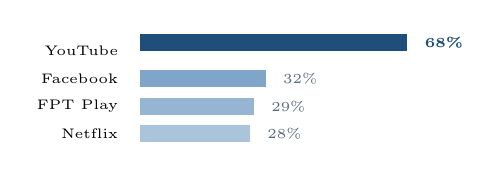
\begin{tikzpicture}[bar/.style={rounded corners=1pt}]
  \node[anchor=east, font=\tiny] at (0,0) {YouTube};
  \fill[BKTemplate] (0.15,0) rectangle +(3.4,0.22);
  \node[anchor=west, font=\tiny\bfseries, text=BKTemplate] at (3.65,0.11) {68\%};
  \node[anchor=east, font=\tiny] at (0,-0.35) {Facebook};
  \fill[BKLight!60] (0.15,-0.46) rectangle +(1.6,0.22);
  \node[anchor=west, font=\tiny, text=TextGray] at (1.85,-0.35) {32\%};
  \node[anchor=east, font=\tiny] at (0,-0.70) {FPT Play};
  \fill[BKLight!50] (0.15,-0.81) rectangle +(1.45,0.22);
  \node[anchor=west, font=\tiny, text=TextGray] at (1.70,-0.70) {29\%};
  \node[anchor=east, font=\tiny] at (0,-1.05) {Netflix};
  \fill[BKLight!40] (0.15,-1.16) rectangle +(1.4,0.22);
  \node[anchor=west, font=\tiny, text=TextGray] at (1.65,-1.05) {28\%};
\end{tikzpicture}\\[2pt]
{\scriptsize\color{TextGray} Số người dùng: YouTube 62,1tr $\cdot$ TikTok 76,1tr (18+)}
\end{block}
\vspace{1pt}
\begin{block}{Âm nhạc}
{\scriptsize\color{TextGray} Nghe nhạc (Decision Lab Q1/2024)}\\[1pt]
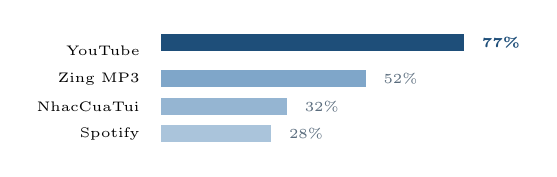
\begin{tikzpicture}[bar/.style={rounded corners=1pt}]
  \node[anchor=east, font=\tiny] at (0,0) {YouTube};
  \fill[BKTemplate] (0.15,0) rectangle +(3.85,0.22);
  \node[anchor=west, font=\tiny\bfseries, text=BKTemplate] at (4.10,0.11) {77\%};
  \node[anchor=east, font=\tiny] at (0,-0.35) {Zing MP3};
  \fill[BKLight!60] (0.15,-0.46) rectangle +(2.6,0.22);
  \node[anchor=west, font=\tiny, text=TextGray] at (2.85,-0.35) {52\%};
  \node[anchor=east, font=\tiny] at (0,-0.70) {NhacCuaTui};
  \fill[BKLight!50] (0.15,-0.81) rectangle +(1.6,0.22);
  \node[anchor=west, font=\tiny, text=TextGray] at (1.85,-0.70) {32\%};
  \node[anchor=east, font=\tiny] at (0,-1.05) {Spotify};
  \fill[BKLight!40] (0.15,-1.16) rectangle +(1.4,0.22);
  \node[anchor=west, font=\tiny, text=TextGray] at (1.65,-1.05) {28\%};
\end{tikzpicture}
\end{block}
\end{column}
% ================= RIGHT: NEWS + GAME =================
\begin{column}{0.48\textwidth}
\begin{block}{Tin tức}
\begin{itemize}\setlength{\itemsep}{1pt}
\item Báo riêng: VnExpress, Tuổi Trẻ, Dân trí
\item Tổng hợp: Báo Mới~--~tin từ hơn \textbf{150} báo điện tử
\end{itemize}
\end{block}
\vspace{1pt}
\begin{block}{Minigame}
\begin{tikzpicture}
  % Hai chỉ số: số đậm ở trên, chú thích ngay bên dưới (neo tây-bắc, chảy xuống)
  \node[anchor=north west, font=\footnotesize\bfseries, text=BKTemplate] at (0,1.95) {1,29 tỷ};
  \node[anchor=north west, font=\tiny, text=TextGray, text width=2.5cm, align=left] at (0,1.60)
    {lượt tải game di động 2025 (Adjust)};
  \node[anchor=north west, font=\footnotesize\bfseries, text=BKTemplate] at (3.55,1.95) {33 phút};
  \node[anchor=north west, font=\tiny, text=TextGray, text width=2.3cm, align=left] at (3.55,1.60)
    {phiên chơi game trung bình, Q1/2026};
  % Badge tăng trưởng
  \node[draw=GreenOK, fill=GreenOK!10, rounded corners=3pt, font=\tiny\bfseries, text=GreenOK!70!black, inner sep=2.5pt, anchor=west] at (0,0.50) {+15\% Q1/2026};
  \node[anchor=west, font=\tiny, text=TextGray] at (1.80,0.50) {số phiên chơi, so cùng kỳ (Adjust)};
\end{tikzpicture}
\end{block}
\end{column}
\end{columns}
\end{frame}

% ------------------------------------------------------------
\subsection{Đối thủ}
% ------------------------------------------------------------
\begin{frame}{Đối thủ trực tiếp: Những nền tảng đã gộp nhiều nội dung}
\footnotesize
\begin{columns}[T]
\begin{column}{0.32\textwidth}
\centering

\includegraphics[height=1.6cm,width=3.0cm,keepaspectratio=true]{figures/Đối thủ-Youtube.png}\\[2pt]
\begin{block}{\scriptsize\bfseries YouTube}
\begin{itemize}\setlength{\itemsep}{2pt}
\item Hệ sinh thái video lớn nhất
\item Premium: chạy nền, ngoại tuyến
\item Playables: chơi minigame nhẹ trong app
\end{itemize}
\end{block}
\end{column}
\begin{column}{0.32\textwidth}
\centering

\includegraphics[height=1.6cm,width=3.0cm,keepaspectratio=true]{figures/Đối thủ-Tiktok.png}\\[2pt]
\begin{block}{\scriptsize\bfseries TikTok}
\begin{itemize}\setlength{\itemsep}{2pt}
\item Video ngắn số 1
\item Minigame trong app
\item TikTok Music đóng cửa 28/11/2024 (5 thị trường, không gồm Việt Nam)
\end{itemize}
\end{block}
\end{column}
\begin{column}{0.32\textwidth}
\centering

\includegraphics[height=1.6cm,width=3.0cm,keepaspectratio=true]{figures/Đối thủ-Mocha.png}\\[2pt]
\begin{block}{\scriptsize\bfseries Mocha}
\begin{itemize}\setlength{\itemsep}{2pt}
\item Siêu ứng dụng liên lạc \& giải trí
\item Data miễn phí cho thuê bao Viettel
\item Nghe nhạc, xem video, xem phim, livestream, game
\end{itemize}
\end{block}
\end{column}
\end{columns}
\end{frame}

% ------------------------------------------------------------
\begin{frame}{Đối thủ gián tiếp: Mỗi app một phân hệ}
\footnotesize
\begin{columns}[T]
\begin{column}{0.48\textwidth}
\begin{block}{Âm nhạc}
Spotify, Zing MP3, NhacCuaTui --- mỗi app giữ một mảnh ghép
\end{block}
\vspace{1pt}
\begin{block}{Video}
Netflix, FPT Play --- nền tảng video chuyên biệt
\end{block}
\end{column}
\begin{column}{0.48\textwidth}
\begin{block}{Tin tức}
VnExpress, Tuổi Trẻ, Báo Mới --- mỗi app một nguồn tin
\end{block}
\vspace{1pt}
\begin{block}{Minigame}
Shopee (quiz, ticket game) --- gamification trong app thương mại
\end{block}
\end{column}
\end{columns}
\end{frame}

% ------------------------------------------------------------
\begin{frame}{Đối thủ: Ma trận tính năng}
\small
\centering
\begin{tabular}{@{}p{2.3cm}cccc@{}}
\toprule
\textbf{Ứng dụng} & \textbf{Video} & \textbf{Nhạc} & \textbf{Tin tức} & \textbf{Minigame} \\
\midrule
YouTube & \cmark & \pmark$^{\text{\tiny Premium}}$ & \xmark & \pmark$^{\text{\tiny Playables}}$ \\
TikTok & \cmark & \pmark$^{\text{\tiny qua sound}}$ & \xmark & \pmark \\
Mocha & \cmark & \cmark$^{\text{\tiny Keeng}}$ & \cmark & \cmark \\
Spotify/Zing & \xmark & \cmark & \pmark$^{\text{\tiny podcast}}$ & \xmark \\
Báo Mới & \xmark & \xmark & \cmark & \xmark \\
Shopee & \xmark & \xmark & \xmark & \pmark$^{\text{\tiny quiz}}$ \\
\midrule
\rowcolor{LightBG}
\textbf{Đề xuất} & \textbf{\cmark} & \textbf{\cmark} & \textbf{\cmark} & \textbf{\cmark} \\
\bottomrule
\end{tabular}

\vspace{0.12cm}
{\scriptsize \cmark~có \quad \pmark~một phần / kèm điều kiện \quad \xmark~không có}

\vspace{0.12cm}
\begin{block}{Khoảng trống}
\footnotesize Mocha hướng tới đủ bốn loại nội dung nhưng \textbf{không liên kết} chúng với nhau; các ứng dụng còn lại mỗi app một phân hệ. Không ai cho nội dung \textbf{phối hợp với nhau}.
\end{block}
\end{frame}

% ------------------------------------------------------------
\subsection{SWOT}
% ------------------------------------------------------------
\begin{frame}{SWOT}
\begin{center}
\begin{tikzpicture}[
    qbodys/.style={rounded corners=4pt, draw=GreenOK!70, fill=GreenOK!6, thick},
    qbodyw/.style={rounded corners=4pt, draw=OrangeWarn!70, fill=OrangeWarn!6, thick},
    qbodyo/.style={rounded corners=4pt, draw=BKLight!70, fill=BKLight!6, thick},
    qbodyt/.style={rounded corners=4pt, draw=RedNo!70, fill=RedNo!6, thick},
    qhead/.style={rounded corners=3pt}]
  \begin{scope}[shift={(0,3.15)}]
    \draw[qbodys] (0,0) rectangle (6.7,2.95);
    \fill[GreenOK,qhead] (0.07,2.42) rectangle (6.63,2.88);
    \node[anchor=west, font=\scriptsize\bfseries, text=white] at (0.3,2.65) {S~--~Điểm mạnh};
    \node[anchor=north west, text width=6.1cm, align=left, font=\tiny] at (0.3,2.28) {%
      \begin{itemize}\itemsep2pt
        \item[S1] Một tài khoản cho bốn phân hệ; nhạc không ngắt khi chuyển tab
        \item[S2] Playlist trộn nhạc, video, tin; chuyển nội dung sang dạng nghe
        \item[S3] Minigame từ nội dung: đố tin, đoán bài hát, karaoke
        \item[S4] Gamification chung: nhiệm vụ, streak, thú ảo
      \end{itemize}};
  \end{scope}
  \begin{scope}[shift={(6.9,3.15)}]
    \draw[qbodyw] (0,0) rectangle (6.7,2.95);
    \fill[OrangeWarn,qhead] (0.07,2.42) rectangle (6.63,2.88);
    \node[anchor=west, font=\scriptsize\bfseries, text=white] at (0.3,2.65) {W~--~Điểm yếu};
    \node[anchor=north west, text width=6.1cm, align=left, font=\tiny] at (0.3,2.28) {%
      \begin{itemize}\itemsep2pt
        \item[W1] Kho nội dung nhỏ; không ngân sách mua bản quyền
        \item[W2] Phân hệ nông hơn ứng dụng chuyên biệt, nhất là gợi ý
        \item[W3] Gộp bốn phân hệ tăng dung lượng, chậm khởi động
        \item[W4] Thương hiệu mới, nhóm nhỏ, thời gian có hạn
      \end{itemize}};
  \end{scope}
  \begin{scope}[shift={(0,0)}]
    \draw[qbodyo] (0,0) rectangle (6.7,2.95);
    \fill[BKLight,qhead] (0.07,2.42) rectangle (6.63,2.88);
    \node[anchor=west, font=\scriptsize\bfseries, text=white] at (0.3,2.65) {O~--~Cơ hội};
    \node[anchor=north west, text width=6.1cm, align=left, font=\tiny] at (0.3,2.28) {%
      \begin{itemize}\itemsep2pt
        \item[O1] 85,6 triệu người dùng Internet, mạng tốc độ cao
        \item[O2] Retention giải trí chỉ 1\% sau 30 ngày~--~vấn đề chung
        \item[O3] Gamification quen thuộc qua MoMo, Shopee
        \item[O4] YouTube nền cần Premium; TikTok Music đã đóng
      \end{itemize}};
  \end{scope}
  \begin{scope}[shift={(6.9,0)}]
    \draw[qbodyt] (0,0) rectangle (6.7,2.95);
    \fill[RedNo,qhead] (0.07,2.42) rectangle (6.63,2.88);
    \node[anchor=west, font=\scriptsize\bfseries, text=white] at (0.3,2.65) {T~--~Thách thức};
    \node[anchor=north west, text width=6.1cm, align=left, font=\tiny] at (0.3,2.28) {%
      \begin{itemize}\itemsep1pt
        \item[T1] Đối thủ lớn đã có minigame, sao chép nhanh
        \item[T2] Bản quyền nhạc, video; tổng hợp tin cần giấy phép
        \item[T3] Điểm thưởng không được quy đổi ra tiền
        \item[T4] Luật BVDLCN 2025 chặt hơn về đồng ý
        \item[T5] Người dùng ngại rời playlist, lịch sử cũ
      \end{itemize}};
  \end{scope}
\end{tikzpicture}
\end{center}
\end{frame}

% ------------------------------------------------------------
\subsection{User Personas}
% ------------------------------------------------------------
\begin{frame}{User Personas (1/3)}
\linespread{0.88}%
\begin{columns}[T]
\begin{column}{0.48\textwidth}
\begin{block}{\small Minh Anh~--~21, sinh viên \tiny(Primary)}
{\tiny\color{TextGray} 21, sinh viên đại học $\cdot$ TP.\ HCM $\cdot$ công nghệ cao $\cdot$ Android 6~GB $\cdot$ 3--5 giờ/ngày}\par\vspace{0.6mm}
{\tiny\textbf{Mục tiêu:} dùng nhiều loại nội dung trong một app; xem video khi đọc tin; nghe nhạc khi lướt tin hoặc chơi game; chuyển đổi nhanh; giảm số lần mở/đóng app}\par\vspace{0.4mm}
{\tiny\textbf{Pain:} liên tục chuyển app; nội dung bị dừng khi đổi hoạt động; khó tìm lại video/bài đang xem; PIP che nội dung; âm thanh chồng nhau}\par\vspace{0.4mm}
{\tiny\textbf{Hành vi:} giải trí giờ nghỉ và buổi tối; quen vuốt, chạm, kéo thả; thích nội dung tiếp tục từ chỗ cũ; thường làm một việc chính + một việc phụ}\par\vspace{0.4mm}
{\tiny\textbf{Tình huống:} Đang xem video, muốn đọc bài báo mới. Chạm tab Tin $\rightarrow$ video tự thu PIP, kéo sang góc khác khỏi đoạn văn. Đọc xong, chạm PIP quay lại video phát tiếp đúng vị trí.}
\end{block}
\end{column}
\begin{column}{0.48\textwidth}
\begin{block}{\small Hoàng Nam~--~27, nhân viên văn phòng}
{\tiny\color{TextGray} 27, nhân viên văn phòng $\cdot$ TP.\ HCM $\cdot$ công nghệ TB--khá $\cdot$ Android 8~GB $\cdot$ 1--2 giờ/ngày}\par\vspace{0.6mm}
{\tiny\textbf{Mục tiêu:} đọc nhanh tin trong giờ nghỉ; nghe nhạc khi di chuyển; tiếp tục bài viết trước đó bằng ít thao tác; điều khiển âm thanh từ notification hoặc màn hình khoá}\par\vspace{0.4mm}
{\tiny\textbf{Pain:} không có thời gian tìm nội dung; thao tác nhiều màn gây bất tiện; âm thanh gián đoạn khi có cuộc gọi; phải tìm lại bài đang nghe/đọc; giao diện nhiều tùy chọn gây rối}\par\vspace{0.4mm}
{\tiny\textbf{Hành vi:} dùng khi di chuyển, nghỉ trưa, sau giờ làm; nghe nhạc qua tai nghe Bluetooth; thói quen khoá màn khi nghe; thích nút điều khiển rõ ràng}\par\vspace{0.4mm}
{\tiny\textbf{Tình huống:} Trên đường đến công ty, phát playlist rồi khoá điện thoại. Nghỉ trưa mở app đọc tin, nhạc vẫn phát, điều khiển qua dock. Có cuộc gọi, app tự nhường; sau cuộc gọi nhạc phát lại đúng chỗ.}
\end{block}
\end{column}
\end{columns}
\end{frame}

% ------------------------------------------------------------
\begin{frame}{User Personas (2/3)}
\linespread{0.88}%
\begin{columns}[T]
\begin{column}{0.48\textwidth}
\begin{block}{\small Quốc Huy~--~19, sinh viên năm nhất}
{\tiny\color{TextGray} 19, sinh viên năm nhất $\cdot$ Bình Dương $\cdot$ công nghệ trung bình $\cdot$ Android 3~GB $\cdot$ dữ liệu giới hạn}\par\vspace{0.6mm}
{\tiny\textbf{Mục tiêu:} chơi minigame đơn giản; nghe nhạc khi chơi game; chơi tiếp khi mất mạng; không mất tiến độ; hạn chế giật lag; tiết kiệm dữ liệu}\par\vspace{0.4mm}
{\tiny\textbf{Pain:} máy chậm khi nhiều tác vụ; mạng không ổn định; game mất tiến độ khi app bị đóng; video HQ tốn dữ liệu; âm game xung đột nhạc nền}\par\vspace{0.4mm}
{\tiny\textbf{Hành vi:} chơi game giờ nghỉ; ưu tiên game nhẹ, ngắn; mở nhạc khi chơi; chọn chất lượng thấp để tiết kiệm data}\par\vspace{0.4mm}
{\tiny\textbf{Tình huống:} Đang nghe nhạc, vào Games mở 2048. Nhạc vẫn phát, âm game tự nhỏ nhường nhạc. Mạng ngắt nhưng game vẫn chạy offline. Chuyển sang Tin đọc bài đã lưu, app tạm dừng game giữ ván dở. Quay lại, ván dở tự hiện lại.}
\end{block}
\end{column}
\begin{column}{0.48\textwidth}
\begin{block}{\small Thảo Vy~--~24, nhân viên marketing}
{\tiny\color{TextGray} 24, nhân viên marketing $\cdot$ TP.\ HCM $\cdot$ công nghệ cao $\cdot$ Android 8~GB $\cdot$ Wi-Fi + 5G}\par\vspace{0.6mm}
{\tiny\textbf{Mục tiêu:} khám phá nội dung mới; chuyển đổi giữa video và bài báo cùng chủ đề; tìm kiếm trên nhiều phân hệ; lưu nội dung xem sau; tiếp tục từ chỗ cũ}\par\vspace{0.4mm}
{\tiny\textbf{Pain:} nội dung cùng chủ đề nằm rải rác trên nhiều app; phải tìm lại chủ đề khi chuyển video sang tin; khó quản lý danh sách xem sau; dễ mất dấu nội dung đã xem}\par\vspace{0.4mm}
{\tiny\textbf{Hành vi:} xem video, đọc báo, tìm chủ đề mới; hay dùng search và bộ lọc; chuyển từ nội dung này sang nội dung liên quan}\par\vspace{0.4mm}
{\tiny\textbf{Tình huống:} Đang đọc bài báo về công nghệ mới. Muốn xem video liên quan, dùng Search xuyên nội dung. Vị trí đọc được lưu. Xem video xong quay lại Tin, app khôi phục đúng đoạn cũ. Đánh dấu cả bài và video xem cuối tuần.}
\end{block}
\end{column}
\end{columns}
\end{frame}

% ------------------------------------------------------------
\begin{frame}{User Personas (3/3)}
\linespread{0.88}%
\begin{columns}[T]
\begin{column}{0.48\textwidth}
\begin{block}{\small Gia Bảo~--~23, sinh viên CNTT}
{\tiny\color{TextGray} 23, sinh viên CNTT $\cdot$ TP.\ HCM $\cdot$ công nghệ rất cao $\cdot$ Android 12~GB $\cdot$ Wi-Fi + 5G}\par\vspace{0.6mm}
{\tiny\textbf{Mục tiêu:} chủ động chọn cách chuyển tab; điều khiển trạng thái phát; tùy chỉnh vị trí PIP; quyết định giữ video khi vào game; quản lý âm thanh theo từng hoạt động}\par\vspace{0.4mm}
{\tiny\textbf{Pain:} app tự dừng/tiếp tục không đúng ý; không có tùy chọn đổi hành vi chuyển màn; PIP kích thước cố định; khó biết nguồn âm nào đang phát; phải thao tác nhiều để đổi cài đặt}\par\vspace{0.4mm}
{\tiny\textbf{Hành vi:} quen cài đặt nâng cao; trải nghiệm nhiều app đa phương tiện; chấp nhận giao diện phức tạp nếu tổ chức rõ}\par\vspace{0.4mm}
{\tiny\textbf{Tình huống:} Xem video và muốn chơi minigame, đã thiết lập ``giữ PIP khi vào Games''. Mở game, video tự thu nhỏ. Sau đó phát nhạc: app dừng video, ưu tiên bài mới. Quay lại video qua trình điều khiển.}
\end{block}
\end{column}
\begin{column}{0.48\textwidth}
\begin{block}{\small Thu Hà~--~37, nhân viên hành chính}
{\tiny\color{TextGray} 37, nhân viên hành chính $\cdot$ Đồng Nai $\cdot$ công nghệ trung bình $\cdot$ Android 4~GB $\cdot$ Wi-Fi + 4G}\par\vspace{0.6mm}
{\tiny\textbf{Mục tiêu:} đọc tin trên giao diện rõ ràng; điều khiển nhạc bằng nút quen thuộc; biết nội dung nào đang hoạt động; dừng hoặc đóng trình phát bất cứ lúc nào; tăng cỡ chữ khi đọc}\par\vspace{0.4mm}
{\tiny\textbf{Pain:} biểu tượng không nhãn; chữ nhỏ hoặc tương phản thấp; không biết âm phát từ đâu; PIP che nội dung; lo nhấn nhầm mất bài đang đọc}\par\vspace{0.4mm}
{\tiny\textbf{Hành vi:} dùng trong nhà và lúc nghỉ; đọc tin, xem video, nghe nhạc nhiều hơn chơi game; ưu tiên nút bấm rõ hơn cử chỉ; thường dùng một tay}\par\vspace{0.4mm}
{\tiny\textbf{Tình huống:} Mở app đọc bài báo, tăng cỡ chữ bằng nút A+. Mở video liên quan hiện PIP. Muốn tập trung đọc, nhấn ``Tạm dừng video'', app hiển thị video đã dừng, tiếp tục đọc đúng chỗ cũ.}
\end{block}
\end{column}
\end{columns}
\end{frame}

% ------------------------------------------------------------
\subsection{USP \& Winning Zone}
% ------------------------------------------------------------
\begin{frame}{USP \& Winning Zone}
\begin{center}
\begin{tikzpicture}[scale=0.70]
  \begin{scope}
    \clip (0,2.2) circle (2.6);
    \clip (-1.905,-1.1) circle (2.6);
    \fill[AccentGold, opacity=0.35] (-4,-2) rectangle (4,5);
  \end{scope}
  \fill[RedNo, opacity=0.18] (1.905,-1.1) circle (2.6);
  \fill[BKLight, opacity=0.10] (0,2.2) circle (2.6);
  \fill[GreenOK, opacity=0.10] (-1.905,-1.1) circle (2.6);
  \draw[BKLight, very thick] (0,2.2) circle (2.6);
  \draw[GreenOK, very thick] (-1.905,-1.1) circle (2.6);
  \draw[RedNo, very thick] (1.905,-1.1) circle (2.6);
  \node[align=center, font=\small\bfseries, text=BKLight] at (0,3.45) {Nhu cầu\\người dùng};
  \node[align=center, font=\small\bfseries, text=GreenOK!60!black] at (-3.2,-1.6) {Thế mạnh\\đề xuất};
  \node[align=center, font=\small\bfseries, text=RedNo] at (3.2,-1.6) {Thế mạnh\\đối thủ};
  \node[fill=AccentGold!25, draw=black!40, rounded corners=2pt, inner sep=4pt] at (-1.4,0.7) {\small\textbf{Winning Zone}};
\end{tikzpicture}
\end{center}
\vfill
\begin{center}\small
Nhu cầu $\cap$ thế mạnh của đề xuất, \textbf{nằm ngoài} vùng đối thủ đã phủ
\end{center}
\end{frame}

% ------------------------------------------------------------
\begin{frame}{USP \& Winning Zone}
\begin{center}
\begin{tikzpicture}[
    needc/.style={rounded corners=4pt, draw=BKLight!70, fill=BKLight!6, thick},
    ourc/.style={rounded corners=4pt, draw=GreenOK!70, fill=GreenOK!6, thick},
    compc/.style={rounded corners=4pt, draw=RedNo!70, fill=RedNo!6, thick},
    hstrip/.style={rounded corners=3pt}]
  % ---- Nhu cầu người dùng ----
  \begin{scope}[shift={(0,0)}]
    \draw[needc] (0,0) rectangle (4.4,3.4);
    \fill[BKLight,hstrip] (0.07,2.92) rectangle (4.33,3.33);
    \node[anchor=west, font=\scriptsize\bfseries, text=white] at (0.25,3.12) {Nhu cầu người dùng};
    \node[anchor=north west, text width=3.9cm, align=left, font=\tiny] at (0.25,2.78) {%
      \begin{itemize}\itemsep1pt
        \item Chỉ cài và đăng \textbf{một} ứng dụng duy nhất
        \item Chuyển đổi loại nội dung \textbf{không gián đoạn}
        \item Dùng được \textbf{hai loại nội dung song song}
        \item Tiết kiệm dung lượng, RAM và pin
      \end{itemize}};
  \end{scope}
  % ---- Thế mạnh của đề xuất ----
  \begin{scope}[shift={(4.6,0)}]
    \draw[ourc] (0,0) rectangle (4.4,3.4);
    \fill[GreenOK,hstrip] (0.07,2.92) rectangle (4.33,3.33);
    \node[anchor=west, font=\scriptsize\bfseries, text=white] at (0.25,3.12) {Thế mạnh của đề xuất};
    \node[anchor=north west, text width=3.9cm, align=left, font=\tiny] at (0.25,2.78) {%
      \begin{itemize}\itemsep1pt
        \item Bốn phân hệ dùng chung \textbf{một media engine}
        \item \textbf{Dock mini player} xuyên suốt
        \item Song song hai nội dung, popup xác nhận khi xung đột âm thanh
        \item Chuyển đổi hình thức: video $\rightarrow$ mp3, báo $\rightarrow$ audio
        \item Minigame sinh từ nội dung đang xem, điểm thưởng dùng chung
      \end{itemize}};
  \end{scope}
  % ---- Thế mạnh đối thủ ----
  \begin{scope}[shift={(9.2,0)}]
    \draw[compc] (0,0) rectangle (4.4,3.4);
    \fill[RedNo,hstrip] (0.07,2.92) rectangle (4.33,3.33);
    \node[anchor=west, font=\scriptsize\bfseries, text=white] at (0.25,3.12) {Thế mạnh đối thủ};
    \node[anchor=north west, text width=3.9cm, align=left, font=\tiny] at (0.25,2.78) {%
      \begin{itemize}\itemsep1pt
        \item Kho bản quyền lớn (phim HD, Keeng)
        \item Cơ sở người dùng khổng lồ (Mocha 16 triệu)
        \item Data miễn phí thuê bao nhà mạng
        \item Mạng xã hội chat + voice sticker
        \item {\color{TextGray}\itshape Vùng không cạnh tranh trực diện}
      \end{itemize}};
  \end{scope}
\end{tikzpicture}
\end{center}
\vfill
\end{frame}

% ------------------------------------------------------------
\begin{frame}{USP \& Winning Zone}
\small
\centering
\begin{tabular}{@{}p{0.5cm}p{3.4cm}p{8.4cm}@{}}
\toprule
 & \textbf{Nội dung} & \textbf{Biểu hiện cụ thể} \\
\midrule
W1 & Xuyên phân hệ & Dock mini dùng chung 4 loại nội dung; một tài khoản; trạng thái giữ nguyên khi đổi tab \\
W2 & Song song hoá & Nghe nhạc khi đọc tin; PIP video khi lướt; popup xác nhận khi xung đột âm thanh \\
W3 & Converting & Nhấn giữ video $\rightarrow$ trích mp3; bài báo $\rightarrow$ audio ``nghe tin'' \\
W4 & Game gắn nội dung & Đoán bài hát từ kho nhạc; quiz từ bài báo đang đọc \\
W5 & Gamification & Nhiệm vụ, streak, thú cưng, điểm thưởng dùng chung bốn phân hệ \\
W6 & Tổng kết cá nhân & Thẻ tổng kết hoạt động trong tháng, xuất ảnh chia sẻ \\
\bottomrule
\end{tabular}
\end{frame}

% ------------------------------------------------------------
\begin{frame}{Unique Selling Point}
\vspace{2mm}
\begin{exampleblock}{Phát biểu Unique Selling Point}
\small\itshape
Ứng dụng giải trí ``4 trong 1'' trên Android: \textbf{chuyển đổi, chạy song song và chuyển đổi hình thức} giữa video, nhạc, tin tức và minigame trong cùng một app. Ngoài ra có \textbf{hệ thống gamification}: nhiệm vụ mỗi ngày, streak, thú cưng ảo và điểm thưởng dùng chung cho cả bốn phân hệ.
\end{exampleblock}
\vspace{4mm}
\end{frame}

% ============================================================
% SECTION 2 - PHẠM VI SẢN PHẨM
% Tiêu chí chất lượng · Phân loại tính năng (75) · Ma trận chuyển
% Quy tắc âm thanh · Gamification · User Stories · Mockup (ALL 75)
% ============================================================
\section{Phạm vi sản phẩm}

% ------------------------------------------------------------
\subsection{Tiêu chí chất lượng}
% ------------------------------------------------------------
\begin{frame}{Tiêu chí chất lượng}
{\tiny\color{TextGray} Yêu cầu phi chức năng (NFR, non-functional requirements)~--~mỗi tiêu chí có ngưỡng đo được; đo trên máy Android tầm trung, RAM 4~GB, mạng 4G.}
\par\vspace{0.8mm}
\begin{center}\tiny
\begin{tabular}{@{}p{1.0cm}p{3.1cm}p{8.4cm}@{}}
\toprule
\textbf{Mã} & \textbf{Tiêu chí} & \textbf{Ngưỡng đạt} \\
\midrule
UX-01 & Phản hồi thao tác & $\leq$ 100~ms (mốc phản ứng tức thì) \\
UX-02 & Tải nội dung & $\leq$ 3 giây trên mạng 4G \\
UX-03 & Khởi động lạnh & $\leq$ 2 giây; không lần đo nào $\geq$ 5 giây \\
UX-04 & Bắt đầu phát & Video $\leq$ 2 giây, nhạc $\leq$ 1 giây \\
UX-05 & Phát liên tục & $\leq$ 1 lần dừng tải / 10 phút; nhạc không dừng khi chuyển phân hệ \\
UX-06 & Độ mượt & $\geq$ 95\% khung hình $<$ 16~ms; không frozen frame \\
UX-07 & Độ ổn định & Crash $\leq$ 0,5\%, ANR $\leq$ 0,2\% (chặt hơn Android vitals) \\
UX-08 & Số bước thao tác & $\leq$ 3 chạm tới nội dung; chuyển phân hệ 1 chạm \\
UX-09 & Dễ dùng & Hoàn thành tác vụ $\geq$ 90\%; điểm SUS $\geq$ 70 \\
UX-10 & Dung lượng & $\leq$ 50~MB tải về \\
UX-11 & Pin & $\leq$ 5\% / 60 phút phát nhạc nền \\
UX-12 & Accessibility & Vùng chạm $\geq$ 48dp; tương phản $\geq$ 4,5:1 (WCAG AA) \\
UX-13 & Tương thích & Android 8.0+ (API 26), RAM $\geq$ 3~GB \\
UX-14 & Ngôn ngữ & Tiếng Việt mặc định; chuyển ngôn ngữ tức thì \\
\bottomrule
\end{tabular}
\end{center}
\end{frame}

% ------------------------------------------------------------
\begin{frame}{Tiêu chí chất lượng}
\begin{columns}[T]
\begin{column}{0.52\textwidth}
\centering
{\scriptsize\bfseries Bảo mật (SEC)}\\[1mm]
{\tiny\setlength{\tabcolsep}{3pt}
\begin{tabular}{@{}p{0.9cm}p{2.0cm}p{3.5cm}@{}}
\toprule
\textbf{Mã} & \textbf{Tiêu chí} & \textbf{Ngưỡng đạt} \\
\midrule
SEC-01 & Xác thực OTP & 6 chữ số, dùng 1 lần, hiệu lực 5 phút; gửi lại sau 60 giây \\
SEC-02 & Lưu trữ an toàn & Token chỉ nằm trong Android Keystore \\
SEC-03 & Truyền dữ liệu & 100\% request HTTPS, TLS 1.2 trở lên \\
SEC-04 & Quyền truy cập & Xin đúng ngữ cảnh; từ chối vẫn dùng được phần còn lại \\
SEC-05 & Đồng ý dữ liệu & Cá nhân hóa chỉ khi người dùng đồng ý \\
SEC-06 & Xóa tài khoản & Xóa trong app và qua web; hoàn tất trong 20 ngày \\
SEC-07 & Bản ghi giọng hát & Chấm trên thiết bị, xóa ngay sau khi chấm (v2) \\
SEC-08 & Kiểm tra bảo mật & 0 lỗi mức High trước mỗi bản phát hành (MobSF) \\
\bottomrule
\end{tabular}}
\end{column}
\begin{column}{0.46\textwidth}
\centering
{\scriptsize\bfseries Kinh doanh (BIZ)}\\[1mm]
{\tiny\setlength{\tabcolsep}{3pt}
\begin{tabular}{@{}p{0.9cm}p{2.0cm}p{3.0cm}@{}}
\toprule
\textbf{Mã} & \textbf{Tiêu chí} & \textbf{Ngưỡng đạt} \\
\midrule
BIZ-01 & Retention & D1/D7/D30 $\geq$ 16\%/4\%/2\% \\
BIZ-02 & Gắn bó & DAU/MAU $\geq$ 20\% \\
BIZ-03 & Dùng nhiều phân hệ & $\geq$ 40\% người dùng tuần \\
BIZ-04 & Gamification & $\geq$ 30\% DAU hoàn thành $\geq$ 1 nhiệm vụ \\
BIZ-05 & Chuyển đổi Premium & $\geq$ 2\% MAU sau 3 tháng \\
BIZ-06 & Giới hạn quảng cáo & Không hiện khi mở/thoát/đang chơi \\
\bottomrule
\end{tabular}}
\end{column}
\end{columns}
\end{frame}

% ------------------------------------------------------------
\begin{frame}{Tiêu chí chất lượng --- ngoại tuyến và ràng buộc mạng}
\begin{center}
{\tiny
\begin{tabular}{@{}p{1.2cm}p{5.7cm}p{5.7cm}@{}}
\toprule
\textbf{Phân hệ} & \textbf{Khi mất mạng} & \textbf{Khi có mạng lại} \\
\midrule
Video & Đang phát dùng tiếp phần đã đệm; hết đệm thì thông báo chờ kèm nút ``Thử lại'', giữ nguyên vị trí & Người dùng bấm thử lại hoặc tiếp tục theo trạng thái lỗi thật \\
Nhạc & Bài đã tải phát được offline; stream chỉ còn phần đệm & Khôi phục hàng đợi theo chính sách, không dựng engine mới \\
Tin tức & Đọc bài đã lưu trong Room; thiếu cache thì hiện trạng thái rõ ràng & Làm mới từ mạng, ghi vào local rồi mới cập nhật giao diện \\
Trò chơi & Ván cờ và logic cục bộ vẫn chơi được & Đồng bộ điểm theo ID phiên, không ghi đè bản local mới hơn \\
\bottomrule
\end{tabular}}
\end{center}
\vspace{1mm}
\begin{columns}[T]
\begin{column}{0.48\textwidth}
\begin{exampleblock}{\scriptsize Ngân sách tài nguyên}
{\tiny
\begin{itemize}\setlength{\itemsep}{1pt}
\item Tối đa 1 decoder video; fullscreen và floating dùng chung engine
\item Một engine âm thanh dùng chung, không dựng theo từng tab
\item Chỉ game đang hiển thị chạy loop; rời game thì tạm dừng
\item Data Saver: giảm chất lượng / prefetch khi có biến thể phù hợp
\end{itemize}}
\end{exampleblock}
\end{column}
\begin{column}{0.48\textwidth}
\begin{exampleblock}{\scriptsize Quyền truy cập}
{\tiny
\begin{itemize}\setlength{\itemsep}{1pt}
\item INTERNET, FOREGROUND\_SERVICE: khai báo lúc cài, không hỏi
\item RECORD\_AUDIO: xin đúng lúc bấm ghi; từ chối vẫn dùng được phần còn lại
\item Không xin quyền nào lúc mở app lần đầu
\end{itemize}}
\end{exampleblock}
\end{column}
\end{columns}
\end{frame}

% ------------------------------------------------------------
\subsection{Phân loại và ưu tiên tính năng}
% ------------------------------------------------------------
\begin{frame}{Phân loại và ưu tiên tính năng --- 76 tính năng ứng viên}
\begin{columns}[T]
\begin{column}{0.56\textwidth}
\small
\begin{itemize}\setlength{\itemsep}{2pt}
\item \textbf{76 tính năng ứng viên}: Video 18 $\cdot$ Music 14 $\cdot$ News 10 $\cdot$ Games 13 $\cdot$ Dùng chung 21
\item Mỗi tính năng chấm \textbf{Impact (1--5) $\times$ Effort (1--5)}
\end{itemize}
\end{column}
\begin{column}{0.38\textwidth}
\small
\centering
\begin{tabular}{@{}p{3.4cm}p{1.0cm}@{}}
\toprule
\textbf{Nhóm} & \textbf{Số} \\
\midrule
Quick Wins & 32 \\
Major Projects & 27 \\
Fill-ins & 14 \\
Thankless & 3 \\
\bottomrule
\end{tabular}
\end{column}
\end{columns}
\end{frame}

% ------------------------------------------------------------
% 5 bảng tính năng theo phân hệ (FULL, không cắt xén)
% ------------------------------------------------------------
\begin{frame}{Phân loại tính năng: Phân hệ Video (18)}
\begin{center}\tiny
\begin{tabular}{@{}p{1.5cm}p{7.5cm}p{0.3cm}p{0.3cm}p{0.8cm}@{}}
\toprule
\textbf{Mã} & \textbf{Tính năng} & \textbf{I} & \textbf{E} & \textbf{Nhóm} \\
\midrule
\texttt{F-VID-01} & Xem video streaming cơ bản (player HLS/MP4) & 5 & 4 & MP \\
\texttt{F-VID-02} & Feed ``Đề xuất'' theo sở thích & 4 & 3 & MP \\
\texttt{F-VID-03} & Tìm kiếm video & 4 & 2 & QW \\
\texttt{F-VID-04} & Danh sách xem sau (watchlist) & 3 & 1 & QW \\
\texttt{F-VID-05} & Lịch sử xem và tiếp tục từ chỗ dừng & 3 & 1 & QW \\
\texttt{F-VID-06} & Chọn chất lượng phát: Auto hoặc bản 1080p/720p/360p & 4 & 3 & MP \\
\texttt{F-VID-07} & Tải video xem offline & 3 & 4 & TT \\
\texttt{F-VID-08} & Picture-in-picture: video thu nhỏ góc màn hình khi rời trang & 5 & 3 & MP \\
\texttt{F-VID-09} & Chế độ chỉ phát âm thanh của video (audio-only) & 3 & 2 & FI \\
\texttt{F-VID-10} & Nhấn giữ video để trích thành tệp mp3 cho kho cá nhân & 5 & 4 & MP \\
\texttt{F-VID-11} & Chia sẻ link video ra ngoài app & 2 & 1 & FI \\
\texttt{F-VID-12} & Màn hồ sơ nghệ sĩ/kênh: bấm tên để xem mọi nội dung của họ & 3 & 2 & FI \\
\texttt{F-VID-13} & Playlist video theo chủ đề & 3 & 2 & FI \\
\texttt{F-VID-14} & Tua nhanh double-tap và đổi tốc độ phát & 4 & 1 & QW \\
\texttt{F-VID-15} & Gợi ý ``chơi game liên quan video này'': thẻ game cuối video, câu hỏi soạn sẵn lúc đăng nội dung & 4 & 2 & QW \\
\texttt{F-VID-16} & Toàn màn hình: nút ẩn system bars, player chiếm cả trang & 3 & 1 & QW \\
\texttt{F-VID-17} & Điều khiển âm lượng: nút loa mute/unmute + thanh volume hệ thống & 3 & 2 & QW \\
\texttt{F-VID-18} & Pinch-to-zoom cửa sổ nổi: 2 ngón thu phóng 0.5x--2x & 3 & 2 & FI \\
\bottomrule
\end{tabular}
\end{center}
\vfill
{\tiny\color{TextGray} QW = Quick Wins $\cdot$ MP = Major Projects $\cdot$ FI = Fill-ins $\cdot$ TT = Thankless}
\end{frame}

\begin{frame}{Phân loại tính năng: Phân hệ Nhạc (14)}
\begin{center}\tiny
\begin{tabular}{@{}p{1.5cm}p{7.5cm}p{0.3cm}p{0.3cm}p{0.8cm}@{}}
\toprule
\textbf{Mã} & \textbf{Tính năng} & \textbf{I} & \textbf{E} & \textbf{Nhóm} \\
\midrule
\texttt{F-MUS-01} & Player nhạc đầy đủ (phát / dừng / chuyển / tua / repeat / shuffle) & 5 & 3 & MP \\
\texttt{F-MUS-02} & Mini player dock xuyên suốt mọi màn hình & 5 & 3 & MP \\
\texttt{F-MUS-03} & Phát nhạc nền khi rời ứng dụng hoặc khoá màn hình & 5 & 4 & MP \\
\texttt{F-MUS-04} & Tự tạo/sửa/xoá playlist & 4 & 2 & QW \\
\texttt{F-MUS-05} & Hàng phát (queue): thêm tiếp theo, phát cuối, kéo sắp lại & 4 & 2 & QW \\
\texttt{F-MUS-06} & Tìm kiếm nhạc (bài hát/nghệ sĩ/album) & 4 & 2 & QW \\
\texttt{F-MUS-07} & Kho nhạc cá nhân chứa các tệp trích từ video & 4 & 3 & MP \\
\texttt{F-MUS-08} & Gợi ý nhạc theo sở thích & 4 & 3 & MP \\
\texttt{F-MUS-09} & ``Siêu playlist'' (meta-playlist) trộn nhạc và video & 4 & 3 & MP \\
\texttt{F-MUS-10} & Xử lý audio focus: duck/pause khi có luồng âm thanh khác & 5 & 3 & MP \\
\texttt{F-MUS-11} & Equalizer, hiệu chỉnh âm thanh & 2 & 3 & TT \\
\texttt{F-MUS-12} & Tải bài hát offline & 3 & 4 & TT \\
\texttt{F-MUS-13} & Tốc độ phát nhạc: x1/x1.5/x2/x0.5 trên dock và Home card & 3 & 1 & QW \\
\texttt{F-MUS-14} & Lời bài hát: panel scroll trên Now Playing & 3 & 2 & FI \\
\bottomrule
\end{tabular}
\end{center}
\vfill
{\tiny\color{TextGray} QW = Quick Wins $\cdot$ MP = Major Projects $\cdot$ FI = Fill-ins $\cdot$ TT = Thankless}
\end{frame}

\begin{frame}{Phân loại tính năng: Phân hệ Tin tức (10)}
\begin{center}\tiny
\begin{tabular}{@{}p{1.5cm}p{7.5cm}p{0.3cm}p{0.3cm}p{0.8cm}@{}}
\toprule
\textbf{Mã} & \textbf{Tính năng} & \textbf{I} & \textbf{E} & \textbf{Nhóm} \\
\midrule
\texttt{F-NEWS-01} & Feed tin theo chuyên mục và sở thích & 5 & 3 & MP \\
\texttt{F-NEWS-02} & Trình đọc sạch, đổi cỡ chữ & 4 & 2 & QW \\
\texttt{F-NEWS-03} & Lưu bài đọc sau & 3 & 1 & QW \\
\texttt{F-NEWS-04} & Tìm kiếm bài báo & 3 & 2 & FI \\
\texttt{F-NEWS-05} & Chuyển bài báo thành audio (TTS)~--~``nghe tin'' & 5 & 4 & MP \\
\texttt{F-NEWS-06} & Sắp xếp mới nhất / phổ biến & 3 & 1 & QW \\
\texttt{F-NEWS-07} & Nghe nhạc khi đọc tin (dock vẫn phát) & 5 & 1 & QW \\
\texttt{F-NEWS-08} & Quiz sinh ra từ bài báo đang đọc & 4 & 3 & MP \\
\texttt{F-NEWS-09} & Gợi ý bài liên quan & 3 & 2 & FI \\
\texttt{F-NEWS-10} & Bài đang đọc thu nhỏ thành thẻ nổi khi rời tab News & 5 & 3 & MP \\
\bottomrule
\end{tabular}
\end{center}
\vfill
{\tiny\color{TextGray} QW = Quick Wins $\cdot$ MP = Major Projects $\cdot$ FI = Fill-ins $\cdot$ TT = Thankless}
\end{frame}

\begin{frame}{Phân loại tính năng: Phân hệ Trò chơi (13)}
\begin{center}\tiny
\begin{tabular}{@{}p{1.5cm}p{7.5cm}p{0.3cm}p{0.3cm}p{0.8cm}@{}}
\toprule
\textbf{Mã} & \textbf{Tính năng} & \textbf{I} & \textbf{E} & \textbf{Nhóm} \\
\midrule
\texttt{F-GAME-01} & Hub minigame: danh sách, trạng thái mở khoá, phần thưởng & 4 & 2 & QW \\
\texttt{F-GAME-02} & Game đoán bài hát & 5 & 3 & MP \\
\texttt{F-GAME-03} & Quiz tin tức & 4 & 3 & MP \\
\texttt{F-GAME-04} & Quiz kiến thức (kiểu Ai là triệu phú) & 3 & 2 & FI \\
\texttt{F-GAME-05} & Snake -- rắn săn mồi & 3 & 1 & FI \\
\texttt{F-GAME-06} & ``Beat tiles'' -- nốt nhạc rơi theo bài đang phát (kiểu piano tiles) & 4 & 2 & QW \\
\texttt{F-GAME-07} & Bảng xếp hạng tuần/tháng & 4 & 3 & MP \\
\texttt{F-GAME-08} & Chơi game ở nửa dưới màn hình, video chạy phía trên & 4 & 4 & MP \\
\texttt{F-GAME-09} & Phần thưởng khi thắng minigame (điểm) & 5 & 2 & QW \\
\texttt{F-GAME-10} & 2048 (ghép số) & 3 & 2 & FI \\
\texttt{F-GAME-11} & Tic-Tac-Toe (caro 3$\times$3) & 3 & 1 & FI \\
\texttt{F-GAME-12} & Thử thách hằng ngày: xoay vòng 6 game, thưởng 50+5$\times$streak + thức ăn pet & 4 & 2 & QW \\
\texttt{F-GAME-13} & Âm thanh và hiệu ứng game: âm phản hồi thao tác, tự giảm khi có nhạc/video & 3 & 1 & QW \\
\bottomrule
\end{tabular}
\end{center}
\vfill
{\tiny\color{TextGray} QW = Quick Wins $\cdot$ MP = Major Projects $\cdot$ FI = Fill-ins $\cdot$ TT = Thankless}
\end{frame}

\begin{frame}{Phân loại tính năng: Dùng chung (21)}
\begin{center}\tiny
\begin{tabular}{@{}p{1.5cm}p{7.5cm}p{0.3cm}p{0.3cm}p{0.8cm}@{}}
\toprule
\textbf{Mã} & \textbf{Tính năng} & \textbf{I} & \textbf{E} & \textbf{Nhóm} \\
\midrule
\texttt{F-COM-01} & Đăng ký/đăng nhập một tài khoản cho cả 4 phân hệ & 5 & 3 & MP \\
\texttt{F-COM-02} & Onboarding chọn sở thích lần đầu & 4 & 1 & QW \\
\texttt{F-COM-03} & Hồ sơ cá nhân: avatar, khung ảnh theo thành tích & 3 & 2 & FI \\
\texttt{F-COM-04} & Hệ điểm thưởng dùng chung (XP) & 5 & 2 & QW \\
\texttt{F-COM-05} & Nhiệm vụ hằng ngày (3--5 nhiệm vụ) & 4 & 2 & QW \\
\texttt{F-COM-06} & Chuỗi ngày liên tiếp (streak) & 4 & 1 & QW \\
\texttt{F-COM-07} & Thú cưng ảo: nuôi bằng điểm, tiến hoá theo mốc & 4 & 3 & MP \\
\texttt{F-COM-08} & Huy hiệu thành tựu & 3 & 2 & FI \\
\texttt{F-COM-09} & Khung avatar độc quyền theo mốc thành tích & 3 & 1 & QW \\
\texttt{F-COM-10} & Tổng kết tháng kiểu ``wrapped'', xuất thẻ chia sẻ & 4 & 3 & MP \\
\texttt{F-COM-11} & Tìm kiếm xuyên nội dung (một ô tìm cho 4 phân hệ) & 4 & 3 & MP \\
\texttt{F-COM-12} & Nhắc nhiệm vụ/streak hằng ngày & 3 & 1 & QW \\
\texttt{F-COM-13} & Cài đặt: sáng/tối, ngôn ngữ, tiết kiệm dữ liệu & 4 & 2 & QW \\
\texttt{F-COM-14} & Cửa sổ xác nhận khi hai luồng âm thanh xung đột & 5 & 2 & QW \\
\texttt{F-COM-15} & Cửa hàng đổi quà bằng điểm (mở game, đồ pet, khung avatar) & 4 & 2 & QW \\
\texttt{F-COM-16} & Chế độ ngoại tuyến cơ bản: tin đã lưu, trạng thái mất mạng & 3 & 3 & MP \\
\texttt{F-COM-17} & Báo nội dung không phù hợp & 2 & 1 & FI \\
\texttt{F-COM-18} & Chế độ khách dùng thử (không cần tài khoản) & 3 & 2 & QW \\
\texttt{F-COM-19} & Karaoke/Record: ghi màn hình video (MediaProjection), countdown 3-2-1 & 4 & 4 & MP \\
\texttt{F-COM-20} & Vuốt ngang đổi phân hệ (trừ Games) + hoàn tác đóng nhạc & 3 & 2 & QW \\
\texttt{F-COM-21} & Ghi âm, hát karaoke cùng bài hát đang phát (bên Nhạc) & 4 & 3 & MP \\
\bottomrule
\end{tabular}
\end{center}
\vfill
{\tiny\color{TextGray} QW = Quick Wins $\cdot$ MP = Major Projects $\cdot$ FI = Fill-ins $\cdot$ TT = Thankless}
\end{frame}

% ------------------------------------------------------------
\subsection{Sơ đồ use case}
% ------------------------------------------------------------
\begin{frame}{Sơ đồ use case tổng quan}
\begin{center}
\begin{tikzpicture}[
  font=\tiny,
  uc/.style={ellipse, draw=BKTemplate, thick, fill=white, inner sep=0.5pt, align=center},
  act/.style={draw=black!70, thick},
  lnk/.style={draw=black!35},
  rel/.style={draw=black!65, dashed, thick, -{Latex[open, length=1.6mm]}}]
  % ===== Ranh giới hệ thống =====
  \draw[draw=BKTemplate!60, thick, rounded corners=4pt] (2.45,2.05) rectangle (14.3,7.05);
  \node[font=\scriptsize\bfseries\color{BKTemplate}] at (8.35,7.2) {OneSpace};
  % ===== Nhãn cụm =====
  \node[font=\tiny\bfseries\color{TextGray}] at (3.55,6.82) {VIDEO};
  \node[font=\tiny\bfseries\color{TextGray}] at (5.95,6.82) {NHẠC};
  \node[font=\tiny\bfseries\color{TextGray}] at (8.35,6.82) {TIN TỨC};
  \node[font=\tiny\bfseries\color{TextGray}] at (10.75,6.82) {TRÒ CHƠI};
  \node[font=\tiny\bfseries\color{TextGray}] at (13.15,6.82) {THƯỞNG};
  \node[font=\tiny\bfseries\color{TextGray}] at (8.9,3.32) {NỀN TẢNG \& DÙNG CHUNG};
  % ===== Tác nhân =====
  \draw[act] (1.0,4.98) circle (0.13);
  \draw[act] (1.0,4.85) -- (1.0,4.48);
  \draw[act] (0.83,4.68) -- (1.17,4.68);
  \draw[act] (1.0,4.48) -- (0.85,4.26);
  \draw[act] (1.0,4.48) -- (1.15,4.26);
  \node[align=center, font=\tiny\bfseries] at (1.0,4.0) {Người\\dùng};
  % ===== Association: tác nhân → 12 UC mục tiêu (vẽ trước, ellipse che sau) =====
  \draw[lnk] (1.17,4.68) -- (3.55,6.15);
  \draw[lnk] (1.17,4.68) -- (5.95,6.15);
  \draw[lnk] (1.17,4.68) -- (8.35,6.15);
  \draw[lnk] (1.17,4.68) -- (10.75,6.15);
  \draw[lnk] (1.17,4.68) -- (13.15,6.15);
  \draw[lnk] (1.17,4.68) -- (13.15,4.95);
  \draw[lnk] (1.17,4.68) -- (13.15,3.75);
  \draw[lnk] (1.17,4.68) -- (5.95,3.75);
  \draw[lnk] (1.17,4.68) -- (4.3,2.65);
  \draw[lnk] (1.17,4.68) -- (7.0,2.65);
  \draw[lnk] (1.17,4.68) -- (9.7,2.65);
  \draw[lnk] (1.17,4.68) -- (12.4,2.65);
  % ===== Quan hệ then chốt: «extend» (biến thể → cơ sở) =====
  \draw[rel] (3.55,4.52) -- (3.55,5.72);
  \draw[rel] (5.95,4.52) -- (5.95,5.72);
  \draw[rel] (5.35,5.15) -- (4.2,5.78);
  % ===== UC mục tiêu (12) + biến thể then chốt (2) =====
  \node[uc] at (3.55,6.15) {Xem video\\{\color{TextGray}(UC-02)}};
  \node[uc] at (5.95,6.15) {Nghe nhạc\\{\color{TextGray}(UC-03)}};
  \node[uc] at (8.35,6.15) {Đọc tin\\{\color{TextGray}(UC-04)}};
  \node[uc] at (10.75,6.15) {Chơi minigame\\{\color{TextGray}(UC-05)}};
  \node[uc] at (13.15,6.15) {Theo dõi tiến độ\\\& thành tích\\{\color{TextGray}(UC-06)}};
  \node[uc] at (3.55,4.95) {Tiếp tục xem khi\\chuyển phân hệ\\{\color{TextGray}(X1)}};
  \node[uc] at (5.95,4.95) {Xử lý xung đột\\âm thanh\\{\color{TextGray}(X0)}};
  \node[uc] at (13.15,4.95) {Chăm sóc\\thú cưng\\{\color{TextGray}(UC-07)}};
  \node[uc] at (5.95,3.75) {Ghi âm karaoke\\{\color{TextGray}(UC-12)}};
  \node[uc] at (13.15,3.75) {Đổi quà\\{\color{TextGray}(UC-08)}};
  \node[uc] at (4.3,2.65) {Vào ứng dụng \&\\chọn sở thích\\{\color{TextGray}(UC-01)}};
  \node[uc] at (7.0,2.65) {Lưu nội dung\\để dùng sau\\{\color{TextGray}(UC-09)}};
  \node[uc] at (9.7,2.65) {Tìm nội dung\\{\color{TextGray}(UC-10)}};
  \node[uc] at (12.4,2.65) {Quản lý danh tính\\{\color{TextGray}(UC-11)}};
  % ===== Legend =====
  \draw[rel] (2.75,2.16) -- (3.5,2.16);
  \node[font=\tiny, text=TextGray, anchor=west] at (3.6,2.16) {\guillemotleft extend\guillemotright{} = biến thể có điều kiện};
\end{tikzpicture}
\end{center}
\vspace{0.3mm}
{\tiny\color{TextGray} 76 tính năng $\rightarrow$ \textbf{12 UC mục tiêu} (động từ + danh từ), tách \textbf{8 «extend»} + \textbf{4 «include»} ở slide sau. Một tác nhân: chế độ khách/đăng nhập không đổi năng lực (hiện thực demo).}
\end{frame}

% ------------------------------------------------------------
\subsection{Quan hệ giữa các use case}
% ------------------------------------------------------------
\begin{frame}{Quan hệ use case: «extend» và «include»}
\begin{center}\tiny
\setlength{\tabcolsep}{3pt}
\begin{tabular}{@{}p{0.65cm}p{3.1cm}p{1.35cm}p{3.4cm}p{4.1cm}@{}}
\toprule
\textbf{Mã} & \textbf{Use case} & \textbf{Loại} & \textbf{Cơ sở · điều kiện} & \textbf{Hiện thực} \\
\midrule
\multicolumn{5}{@{}l}{\itshape «extend» --- biến thể có điều kiện} \\
X0 & Xử lý xung đột âm thanh & extend & UC-02, UC-03 · [2 luồng tiếng] & SessionPolicy; popup C1/C2 + rule nhớ \\
X1 & Tiếp tục xem (thu nhỏ) & extend & UC-02 · [rời màn player, trừ Home/Games] & FloatingVideo trong shell, cùng engine \\
X2 & Nghe âm thanh video & extend & UC-02 · [chọn tai nghe] & AudioOnlyState; lưu vị trí \\
X3 & Quiz cuối video & extend & UC-02 · [video kết thúc, không playlist] & CTA trong player; cộng điểm \\
X4 & Nghe tin TTS & extend & UC-04 · [bấm tai nghe] & TTS on-device (demo thu) \\
X5 & Kiểm tra nhanh cuối bài & extend & UC-04 · [bài có quiz] & Quiz card; +15 điểm/câu \\
X6 & Thử thách hằng ngày & extend & UC-05 · [có thử thách chưa xong] & 1 template/ngày; 50+5×streak \\
X7 & Vừa chơi vừa xem video & extend & UC-05 · [video đang phát] & Chia 34/66; 2 game toàn màn \\
X8 & Đọc nổi & extend & UC-04 · [rời reader khi đang mở bài] & Thẻ đọc nổi; ẩn trong game \\
\midrule
\multicolumn{5}{@{}l}{\itshape «include» --- hành vi bắt buộc dùng chung} \\
I1 & Khôi phục vị trí xem & include & UC-02 · mỗi lần mở video & Room checkpoint 3 giây, lệch $\leq$ 2 giây \\
I2 & Duy trì hàng đợi & include & UC-03 · khi phát & Engine queue + tự chuyển bài \\
I3 & Ghi nhận điểm \& nhiệm vụ & include & UC-05 · sau khi kết thúc ván & Room; +20/nhiệm vụ; mở pet \\
I4 & Xác thực OTP & include & UC-11 · khi đăng nhập OTP & Demo: mã 123456, hạn 5 phút \\
\midrule
\multicolumn{5}{@{}l}{\itshape Use case hỗ trợ} \\
UC-13 & Tuỳ chỉnh cài đặt & supporting & --- (không include/extend) & 8 nhóm: giao diện, ngôn ngữ, âm thanh\ldots \\
\bottomrule
\end{tabular}
\end{center}
\vspace{0.8mm}
{\tiny\color{TextGray} Mỗi quan hệ có điều kiện kích hoạt và bản ghi hiện thực tương ứng (file:line trong báo cáo).}
\end{frame}

% ------------------------------------------------------------
\subsection{Đặc tả use case mẫu}
% ------------------------------------------------------------
\begin{frame}{Đặc tả use case mẫu --- Xem video (UC-02)}
\begin{columns}[T]
\begin{column}{0.46\textwidth}
{\small\textbf{Thông tin chung}}\\[1.2mm]
{\tiny
\begin{tabular}{@{}p{1.9cm}p{4.6cm}@{}}
\toprule
\textbf{Thuộc tính} & \textbf{Nội dung} \\
\midrule
Mã / tính năng & UC-02 $\cdot$ F-VID-01, 08, 16--18 \\
Tác nhân & Người dùng \\
Tiên điều kiện & Đang ở feed Video; có kết nối \\
Hậu điều kiện & Video phát đúng vị trí đã lưu; phiên giữ khi rời màn; đóng cửa sổ nổi thì lưu Xem sau \\
Truy vết & US-VID-01, US-VID-02, US-CROSS-03; X0, X1, I1; sequence ``video $\rightarrow$ cửa sổ nổi'' \\
\bottomrule
\end{tabular}}
\vspace{1.5mm}

{\scriptsize\color{TextGray} Mẫu đặc tả áp dụng cho 12 UC mục tiêu; mỗi bước đều kiểm thử được (AC ở mục User Stories).}
\end{column}
\begin{column}{0.50\textwidth}
{\small\textbf{Luồng chính}}\\[0.8mm]
{\scriptsize
\begin{enumerate}\setlength{\itemsep}{0.8pt}
\item Chạm một video trong feed
\item Nếu nhạc đang phát: popup 2 lựa chọn + tick nhớ rule (X0)
\item Mở stream tại vị trí đã lưu (I1); phát trong $\leq$ 2 giây
\item Điều khiển: dừng/tua 10s/tốc độ/chất lượng/âm lượng/toàn màn hình
\item Rời màn player: cửa sổ nổi tiếp tục phát, cùng engine (X1)
\item Chạm ``Mở rộng'': quay lại player đúng vị trí
\end{enumerate}}
\vspace{1mm}

{\small\textbf{Luồng thay thế}}\\[0.8mm]
{\scriptsize
\begin{itemize}\setlength{\itemsep}{0.8pt}
\item Đóng cửa sổ nổi: dừng video, lưu vị trí + thêm Xem sau
\item Tab đích là Home: phát trong card feed, không cửa sổ nổi
\item Video kết thúc: hiện quiz cuối video (X3); playlist hỗn hợp tự chuyển bài
\end{itemize}}
\end{column}
\end{columns}
\end{frame}

% ------------------------------------------------------------
\subsection{Ma trận chuyển phân hệ}
% ------------------------------------------------------------
\begin{frame}{Ma trận chuyển phân hệ}
\begin{center}
\begin{tikzpicture}
  % ----- Header cột -----
  \fill[BKTemplate, rounded corners=2pt] (1.75,5.05) rectangle +(2.88,0.42);
  \node[font=\scriptsize\bfseries, text=white] at (3.23,5.26) {Video};
  \fill[BKTemplate, rounded corners=2pt] (4.8,5.05) rectangle +(2.88,0.42);
  \node[font=\scriptsize\bfseries, text=white] at (6.28,5.26) {Music};
  \fill[BKTemplate, rounded corners=2pt] (7.85,5.05) rectangle +(2.88,0.42);
  \node[font=\scriptsize\bfseries, text=white] at (9.32,5.26) {News};
  \fill[BKTemplate, rounded corners=2pt] (10.9,5.05) rectangle +(2.88,0.42);
  \node[font=\scriptsize\bfseries, text=white] at (12.38,5.26) {Games};
  % ----- Header hàng -----
  \fill[BKTemplate, rounded corners=2pt] (0.05,3.9) rectangle +(1.6,1.05);
  \node[font=\scriptsize\bfseries, text=white, rotate=90] at (0.85,4.43) {Video};
  \fill[BKTemplate, rounded corners=2pt] (0.05,2.8) rectangle +(1.6,1.05);
  \node[font=\scriptsize\bfseries, text=white, rotate=90] at (0.85,3.33) {Music};
  \fill[BKTemplate, rounded corners=2pt] (0.05,1.7) rectangle +(1.6,1.05);
  \node[font=\scriptsize\bfseries, text=white, rotate=90] at (0.85,2.23) {News};
  \fill[BKTemplate, rounded corners=2pt] (0.05,0.6) rectangle +(1.6,1.05);
  \node[font=\scriptsize\bfseries, text=white, rotate=90] at (0.85,1.13) {Games};
  % ----- Đường chéo -----
  \fill[TextGray!8, rounded corners=2pt] (1.75,3.9) rectangle +(2.88,1.05);
  \node[font=\tiny, text=TextGray] at (3.19,4.43) {--};
  \fill[TextGray!8, rounded corners=2pt] (4.8,2.8) rectangle +(2.88,1.05);
  \node[font=\tiny, text=TextGray] at (6.24,3.33) {--};
  \fill[TextGray!8, rounded corners=2pt] (7.85,1.7) rectangle +(2.88,1.05);
  \node[font=\tiny, text=TextGray] at (9.29,2.23) {--};
  \fill[TextGray!8, rounded corners=2pt] (10.9,0.6) rectangle +(2.88,1.05);
  \node[font=\tiny, text=TextGray] at (12.34,1.13) {--};
  % ----- Các ô chuyển -----
  \draw[rounded corners=2pt, draw=TextGray!40, fill=white, thick] (4.8,3.9) rectangle +(2.88,1.05);
  \node[anchor=north west, text width=2.68cm, align=left, font=\tiny] at (4.90,4.82) {{\bfseries\textcolor{BKTemplate}{C1}} Video thu nhỏ nổi; hỏi 2 lựa chọn + tick ``Không hỏi lại''};
  \draw[rounded corners=2pt, draw=TextGray!40, fill=white, thick] (7.85,3.9) rectangle +(2.88,1.05);
  \node[anchor=north west, text width=2.68cm, align=left, font=\tiny] at (7.95,4.82) {{\bfseries\textcolor{BKTemplate}{C3}} Video nổi nhãn ``Đang phát''; rời News hiện thẻ ``Đang đọc''};
  \draw[rounded corners=2pt, draw=TextGray!40, fill=white, thick] (10.9,3.9) rectangle +(2.88,1.05);
  \node[anchor=north west, text width=2.68cm, align=left, font=\tiny] at (11.00,4.82) {{\bfseries\textcolor{BKTemplate}{C5}} Chia màn hai phần; video tua và dừng được};
  \draw[rounded corners=2pt, draw=TextGray!40, fill=white, thick] (1.75,2.8) rectangle +(2.88,1.05);
  \node[anchor=north west, text width=2.68cm, align=left, font=\tiny] at (1.85,3.72) {{\bfseries\textcolor{BKTemplate}{C2}} Mở video: hỏi 2 lựa chọn + tick ``Không hỏi lại''};
  \draw[rounded corners=2pt, draw=TextGray!40, fill=white, thick] (7.85,2.8) rectangle +(2.88,1.05);
  \node[anchor=north west, text width=2.68cm, align=left, font=\tiny] at (7.95,3.72) {{\bfseries\textcolor{BKTemplate}{C7}} Nhạc vẫn phát; dock hiện ở mọi tab kể cả trình đọc};
  \draw[rounded corners=2pt, draw=TextGray!40, fill=white, thick] (10.9,2.8) rectangle +(2.88,1.05);
  \node[anchor=north west, text width=2.68cm, align=left, font=\tiny] at (11.00,3.72) {{\bfseries\textcolor{BKTemplate}{C9}} Nhạc vẫn phát; âm game tự giảm, không đè tiếng};
  \draw[rounded corners=2pt, draw=TextGray!40, fill=white, thick] (1.75,1.7) rectangle +(2.88,1.05);
  \node[anchor=north west, text width=2.68cm, align=left, font=\tiny] at (1.85,2.62) {{\bfseries\textcolor{BKTemplate}{C4}} Thẻ ``Đang đọc'' nổi mọi tab (vào game ẩn); chạm quay đúng chỗ};
  \draw[rounded corners=2pt, draw=TextGray!40, fill=white, thick] (4.8,1.7) rectangle +(2.88,1.05);
  \node[anchor=north west, text width=2.68cm, align=left, font=\tiny] at (4.90,2.62) {{\bfseries\textcolor{BKTemplate}{C8}} Thẻ ``Đang đọc'' nổi; quay lại bài bằng một chạm};
  \draw[rounded corners=2pt, draw=TextGray!40, fill=white, thick] (10.9,1.7) rectangle +(2.88,1.05);
  \node[anchor=north west, text width=2.68cm, align=left, font=\tiny] at (11.00,2.62) {{\bfseries\textcolor{BKTemplate}{C11}} Thẻ ``Đang đọc'' nổi; game chạy bình thường};
  \draw[rounded corners=2pt, draw=TextGray!40, fill=white, thick] (1.75,0.6) rectangle +(2.88,1.05);
  \node[anchor=north west, text width=2.68cm, align=left, font=\tiny] at (1.85,1.52) {{\bfseries\textcolor{BKTemplate}{C6}} Ván game tự tạm dừng, giữ ván dở};
  \draw[rounded corners=2pt, draw=TextGray!40, fill=white, thick] (4.8,0.6) rectangle +(2.88,1.05);
  \node[anchor=north west, text width=2.68cm, align=left, font=\tiny] at (4.90,1.52) {{\bfseries\textcolor{BKTemplate}{C10}} Ván tạm dừng; quay lại, ván dở tự hiện lại};
  \draw[rounded corners=2pt, draw=TextGray!40, fill=white, thick] (7.85,0.6) rectangle +(2.88,1.05);
  \node[anchor=north west, text width=2.68cm, align=left, font=\tiny] at (7.95,1.52) {{\bfseries\textcolor{BKTemplate}{C12}} Game tạm dừng, giữ ván dở; rời News thẻ đọc nổi};
\end{tikzpicture}
\end{center}
\vspace{0.3mm}
{\tiny\color{TextGray} Ngoài ma trận: C13~--~nhạc nhường TTS ``Nghe tin'' $\cdot$ C14~--~trích MP3 $\cdot$ C15~--~siêu playlist (case đặc biệt, một chiều).}
\end{frame}

% ------------------------------------------------------------
\subsection{Quy tắc xử lý xung đột âm thanh}
% ------------------------------------------------------------
\begin{frame}{Quy tắc xử lý xung đột âm thanh}
\begin{columns}[T]
\begin{column}{0.54\textwidth}
\footnotesize
\begin{enumerate}\setlength{\itemsep}{4pt}
\item \textbf{Cuộc gọi và báo thức} luôn cao nhất (audio focus của Android); mọi luồng của ứng dụng nhường ngay
\item \textbf{Một nguồn tiếng chính duy nhất}: video mới phát làm nhạc nhường (C2), TTS làm nhạc nhường (C13), âm game tự giảm khi nhạc/video đang chạy (C9)
\item \textbf{Ngoại lệ:} cặp video + nhạc được phát cùng lúc~--~hỏi người dùng (C1) vì cả hai đều là lựa chọn chủ động
\item \textbf{Nhạc dock là luồng nền:} hiện trên mọi tab, nhường khi luồng chính cần tiếng, tiếp tục bằng một chạm
\item \textbf{Không luồng vô hình:} mọi luồng thấy và điều khiển được từ dock mini player
\end{enumerate}
\end{column}
\begin{column}{0.42\textwidth}
\begin{block}{Gián đoạn từ bên ngoài}
{\footnotesize
\begin{itemize}\setlength{\itemsep}{2pt}
\item \textbf{Cuộc gọi:} nhường $\leq$ 0,5~s; sau đó nhạc tự phát lại
\item \textbf{Rút tai nghe:} nhạc và TTS dừng ngay, không phát loa
\item \textbf{Mất mạng:} thử lại sau 5--15~s; game offline chơi tiếp
\item \textbf{App bị đóng:} mở lại khôi phục đủ 4 vị trí trong 2~s
\end{itemize}}
\end{block}
\end{column}
\end{columns}
\end{frame}

% ------------------------------------------------------------
\subsection{Gamification: Vòng lặp giữ chân người dùng}
% ------------------------------------------------------------
\begin{frame}{Gamification: Vòng lặp giữ chân người dùng}
\begin{columns}[T]
\begin{column}{0.48\textwidth}
\footnotesize
\begin{block}{Kiếm điểm}
\begin{itemize}\setlength{\itemsep}{1pt}
\item Nhiệm vụ hằng ngày: \textbf{+20}
\item Quiz cuối video: \textbf{20+5×(combo$-$1)}, max +50
\item Quiz bài báo: \textbf{+15}/câu
\item Quiz kiến thức: thang \textbf{5--60}
\item 2048: score/20, chạm 2048 \textbf{+100}
\item Thắng TTT: Dễ 10 / Vừa 20 / Khó 40
\item Rắn: +2/mồi; Beat Tiles: score/2
\item Đoán bài hát: +10; Trích MP3: +5
\item Thử thách hằng ngày: \textbf{50+5×streak} (max 85)
\end{itemize}
\end{block}
\end{column}
\begin{column}{0.48\textwidth}
\footnotesize
\begin{block}{Tiêu điểm}
\begin{itemize}\setlength{\itemsep}{1pt}
\item Cho thú cưng ăn: \textbf{$-$30}
\item Mở khóa game: Snake 300, Beat Tiles 500
\item Khung avatar: Đồng 200, Bạc 400, Vàng 800
\item Phụ kiện pet: 50--100
\end{itemize}
\end{block}
\vspace{2pt}
\begin{block}{Tiến hoá thú cưng}
\textbf{Trứng} (0đ, nở sau 3 nhiệm vụ) $\rightarrow$ \textbf{Bé cưng} (500đ, gà con vàng)\\
$\rightarrow$ \textbf{Thiếu niên} (2.000đ) $\rightarrow$ \textbf{Trưởng thành} (5.000đ, vẹt)
\end{block}
\vspace{2pt}
\begin{block}{Huy hiệu: 15}
6 huy hiệu hồ sơ + 9 huy hiệu game, có progress bar
\end{block}
\end{column}
\end{columns}
\end{frame}

% ------------------------------------------------------------
\subsection{User Stories}
% ------------------------------------------------------------
\begin{frame}{User Stories --- Khung yêu cầu chức năng}
\small
\begin{itemize}\setlength{\itemsep}{3pt}
\item \textbf{45 user story} kèm acceptance criteria $=$ \textbf{yêu cầu chức năng}
\item Mẫu: ``\textbf{Là} \textit{vai trò}, \textbf{tôi muốn} \textit{hành động}, \textbf{để} \textit{lợi ích}''
\item Điều kiện kiểm tra: ``\textbf{Cho trước / Khi / Thì}''
\item Mức ưu tiên \textbf{Must / Should / Could}; gắn mã tính năng
\end{itemize}
\end{frame}

\begin{frame}{User story kèm Acceptance Criteria}
\linespread{0.9}
{\tiny\color{TextGray} Mỗi story kèm điều kiện kiểm tra mẫu ``\textbf{Cho trước / Khi / Thì}''~--~ba ví dụ tiêu biểu.}
\vspace{1mm}

{\scriptsize\bfseries\color{BKTemplate} US-VID-02}~~{\tiny Must (F-VID-08)}\\
{\tiny Là người dùng đang xem video, tôi muốn video tự thu nhỏ về một góc màn hình khi tôi chuyển sang tab khác, để vừa xem vừa đọc tin hoặc làm việc khác.}\\
{\tiny\textbf{Kiểm tra:} Cho trước video đang phát, khi chuyển sang tab bất kỳ khác, thì video chuyển thành cửa sổ nổi góc màn hình, tiếp tục phát, có ba nút Mở rộng, Tạm dừng và Đóng; chạm Mở rộng phóng to trở lại đúng vị trí.}

\vspace{2mm}
{\scriptsize\bfseries\color{BKTemplate} US-CROSS-05}~~{\tiny Must}\\
{\tiny Là người dùng nhận cuộc gọi, tôi muốn mọi nội dung tự nhường và trở lại đúng chỗ sau cuộc gọi, để không phải tìm lại vị trí cũ.}\\
{\tiny\textbf{Kiểm tra:} Mọi luồng tạm dừng trong 0,5 giây khi có cuộc gọi; sau đó: nhạc tự phát lại, video hiện nút ``Tiếp tục'' từ vị trí sai lệch tối đa 2 giây, game mở lại đúng ván dở; có tuỳ chọn tắt tự phát lại.}

\vspace{2mm}
{\scriptsize\bfseries\color{BKTemplate} US-GAME-02}~~{\tiny Must (F-GAME-02)}\\
{\tiny Là người dùng, tôi muốn chơi game đoán bài hát từ thư viện, để thử thách thấy mình thuộc bài đến đâu.}\\
{\tiny\textbf{Kiểm tra:} Mỗi ván 10 câu, nghe 5 giây rồi chọn 1 trong 4 đáp án; đúng +10 điểm, sai hiện đáp án; hết ván hiện tổng và cộng điểm hệ thống một lần.}

\vfill
{\tiny\color{TextGray} 45/45 story đều có điều kiện kiểm tra dạng này~--~bảng đầy đủ trong báo cáo.}
\end{frame}

% ===== User Stories: Video =====
\begin{frame}{User Stories: Video (1/3)}
\linespread{0.85}
\begin{block}{\scriptsize\bfseries US-VID-01}~~Must \tiny(F-VID-01)
{\scriptsize Là người dùng, tôi muốn chạm một video trong feed và xem ngay trong ứng dụng, để xem video không bị gián đoạn bởi việc chuyển app.}
\end{block}
\vspace{1pt}
\begin{block}{\scriptsize\bfseries US-VID-02}~~Must \tiny(F-VID-08)
{\scriptsize Là người dùng đang xem video, tôi muốn video tự thu nhỏ về một góc màn hình khi tôi chuyển sang tab khác, để vừa xem vừa đọc tin hoặc làm việc khác.}
\end{block}
\vspace{1pt}
\begin{block}{\scriptsize\bfseries US-VID-03}~~Must \tiny(F-VID-14)
{\scriptsize Là người dùng, tôi muốn tua nhanh bằng cú chạm đôi và đổi tốc độ phát, để bỏ qua đoạn không cần xem.}
\end{block}
\vspace{1pt}
\end{frame}

\begin{frame}{User Stories: Video (2/3)}
\linespread{0.85}
\begin{block}{\scriptsize\bfseries US-VID-04}~~Should \tiny(F-VID-02)
{\scriptsize Là người dùng có sở thích riêng, tôi muốn feed video ưu tiên theo chuyên mục tôi chọn, để mở app là thấy nội dung mình muốn.}
\end{block}
\vspace{1pt}
\begin{block}{\scriptsize\bfseries US-VID-05}~~Should \tiny(F-VID-04, F-VID-05)
{\scriptsize Là người dùng, tôi muốn lưu video để xem sau và quay lại đúng chỗ tôi dừng, để không mất dấu nội dung.}
\end{block}
\vspace{1pt}
\begin{block}{\scriptsize\bfseries US-VID-06}~~Should \tiny(F-VID-10)
{\scriptsize Là người dùng, tôi muốn nhấn giữ một video để trích phần âm thanh thành tệp mp3 trong kho nhạc của tôi, để nghe được nội dung đó khi không tiện nhìn màn hình.}
\end{block}
\vspace{1pt}
\end{frame}

\begin{frame}{User Stories: Video (3/3)}
\linespread{0.85}
\begin{block}{\scriptsize\bfseries US-VID-07}~~Could \tiny(F-VID-15)
{\scriptsize Là người dùng thích thử thách, tôi muốn có gợi ý "chơi game liên quan video này" ở cuối video, để giải trí chủ động sau khi xem.}
\end{block}
\vspace{1pt}
\end{frame}

% ===== User Stories: Nhạc =====
\begin{frame}{User Stories: Nhạc (1/3)}
\linespread{0.85}
\begin{block}{\scriptsize\bfseries US-MUS-01}~~Must \tiny(F-MUS-01)
{\scriptsize Là người dùng, tôi muốn chọn một bài từ thư viện và điều khiển phát đầy đủ, để nghe nhạc như ở một ứng dụng nhạc thực thụ.}
\end{block}
\vspace{1pt}
\begin{block}{\scriptsize\bfseries US-MUS-02}~~Must \tiny(F-MUS-02)
{\scriptsize Là người dùng, tôi muốn bài nhạc đang phát hiện thành một dock mini ở mọi màn hình chính, để nghe nhạc trong khi dùng phân hệ khác.}
\end{block}
\vspace{1pt}
\begin{block}{\scriptsize\bfseries US-MUS-03}~~Must \tiny(F-COM-14, F-MUS-10)
{\scriptsize Là người dùng, tôi muốn hệ thống hỏi rõ khi tôi mở một luồng âm thanh khác trong khi đang nghe nhạc, để âm thanh không tự giành nhau gây khó chịu.}
\end{block}
\vspace{1pt}
\end{frame}

\begin{frame}{User Stories: Nhạc (2/3)}
\linespread{0.85}
\begin{block}{\scriptsize\bfseries US-MUS-04}~~Must \tiny(F-MUS-04, F-MUS-05)
{\scriptsize Là người dùng, tôi muốn tự tạo playlist và sắp hàng chờ phát, để nghe nhạc theo trình tự mình muốn.}
\end{block}
\vspace{1pt}
\begin{block}{\scriptsize\bfseries US-MUS-05}~~Should \tiny(F-MUS-07)
{\scriptsize Là người dùng, tôi muốn kho nhạc cá nhân chứa các tệp tôi trích từ video, để quản lý tập trung tại một nơi.}
\end{block}
\vspace{1pt}
\begin{block}{\scriptsize\bfseries US-MUS-06}~~Could \tiny(F-MUS-03)
{\scriptsize Là người dùng, tôi muốn nhạc tiếp tục phát khi tôi rời ứng dụng hoặc khoá màn hình, để nghe nhạc khi làm việc khác.}
\end{block}
\vspace{1pt}
\end{frame}

\begin{frame}{User Stories: Nhạc (3/3)}
\linespread{0.85}
\begin{block}{\scriptsize\bfseries US-MUS-07}~~Could \tiny(F-MUS-06)
{\scriptsize Là người dùng, tôi muốn tìm bài hát theo tên, nghệ sĩ hoặc album, để tới được nội dung mình muốn nhanh hơn là lướt.}
\end{block}
\vspace{1pt}
\end{frame}

% ===== User Stories: Tin tức =====
\begin{frame}{User Stories: Tin tức (1/2)}
\linespread{0.85}
\begin{block}{\scriptsize\bfseries US-NEWS-01}~~Must \tiny(F-NEWS-01)
{\scriptsize Là người dùng, tôi muốn feed tin được sắp theo chuyên mục tôi quan tâm, để cập nhật tin nhanh và đủ.}
\end{block}
\vspace{1pt}
\begin{block}{\scriptsize\bfseries US-NEWS-02}~~Must \tiny(F-NEWS-02)
{\scriptsize Là người dùng đọc lâu, tôi muốn trình đọc sạch và chỉnh cỡ chữ, để đọc không mỏi mắt.}
\end{block}
\vspace{1pt}
\begin{block}{\scriptsize\bfseries US-NEWS-03}~~Must \tiny(F-NEWS-07)
{\scriptsize Là người dùng, tôi muốn vừa đọc bài báo vừa nghe nhạc nền, để không phải chọn giữa hai việc.}
\end{block}
\vspace{1pt}
\end{frame}

\begin{frame}{User Stories: Tin tức (2/2)}
\linespread{0.85}
\begin{block}{\scriptsize\bfseries US-NEWS-04}~~Should \tiny(F-NEWS-05)
{\scriptsize Là người dùng trên đường đi, tôi muốn chuyển một bài báo thành bản audio, để tiếp tục "đọc" tin khi không nhìn được màn hình.}
\end{block}
\vspace{1pt}
\begin{block}{\scriptsize\bfseries US-NEWS-05}~~Should \tiny(F-NEWS-03)
{\scriptsize Là người dùng, tôi muốn lưu bài đọc sau, để đọc đúng lúc mình rảnh.}
\end{block}
\vspace{1pt}
\begin{block}{\scriptsize\bfseries US-NEWS-06}~~Should \tiny(F-NEWS-08, F-GAME-03)
{\scriptsize Là người dùng thích thử thách, tôi muốn một quiz 3 câu hỏi sinh từ bài báo tôi vừa đọc, để vừa đọc vừa chơi và nhận điểm.}
\end{block}
\vspace{1pt}
\end{frame}

% ===== User Stories: Trò chơi =====
\begin{frame}{User Stories: Trò chơi (1/2)}
\linespread{0.85}
\begin{block}{\scriptsize\bfseries US-GAME-01}~~Must \tiny(F-GAME-01)
{\scriptsize Là người dùng, tôi muốn một tab tập hợp các minigame và trạng thái mở khoá, để biết được chơi gì hôm nay.}
\end{block}
\vspace{1pt}
\begin{block}{\scriptsize\bfseries US-GAME-02}~~Must \tiny(F-GAME-02)
{\scriptsize Là người dùng, tôi muốn chơi game đoán bài hát từ thư viện, để thử thách thấy mình thuộc bài đến đâu.}
\end{block}
\vspace{1pt}
\begin{block}{\scriptsize\bfseries US-GAME-03}~~Must \tiny(F-GAME-09)
{\scriptsize Là người dùng, tôi muốn điểm thưởng tích lũy dùng chung cho toàn app, để mọi hoạt động đều có giá trị.}
\end{block}
\vspace{1pt}
\end{frame}

\begin{frame}{User Stories: Trò chơi (2/2)}
\linespread{0.85}
\begin{block}{\scriptsize\bfseries US-GAME-04}~~Could \tiny(F-GAME-08)
{\scriptsize Là người dùng, tôi muốn vừa chơi game vừa xem video trên hai nửa màn hình, để giải trí song song trọn vẹn hai phân hệ.}
\end{block}
\vspace{1pt}
\begin{block}{\scriptsize\bfseries US-GAME-05}~~Could \tiny(F-GAME-07)
{\scriptsize Là người dùng, tôi muốn bảng xếp hạng tuần, để có động lực cạnh tranh.}
\end{block}
\vspace{1pt}
\begin{block}{\scriptsize\bfseries US-GAME-06}~~Should \tiny(F-GAME-05/10)
{\scriptsize Là người dùng, tôi muốn một game phổ biến, khởi động nhanh và không cần biết nội dung (Snake hoặc 2048), để có chỗ vui một phút chờ đợi mà vẫn góp được điểm.}
\end{block}
\vspace{1pt}
\end{frame}

% ===== User Stories: Dùng chung =====
\begin{frame}{User Stories: Dùng chung (1/4)}
\linespread{0.85}
\begin{block}{\scriptsize\bfseries US-COM-01}~~Must \tiny(F-COM-01)
{\scriptsize Là người dùng, tôi muốn đăng ký một tài khoản duy nhất cho cả 4 phân hệ, để không phải quản lý nhiều tài khoản.}
\end{block}
\vspace{1pt}
\begin{block}{\scriptsize\bfseries US-COM-02}~~Must \tiny(F-COM-02)
{\scriptsize Là người dùng mới, tôi muốn chọn nhanh sở thích lần đầu mở app, để nội dung phù hợp với tôi từ đầu.}
\end{block}
\vspace{1pt}
\begin{block}{\scriptsize\bfseries US-COM-03}~~Must \tiny(F-COM-04, 05, 06)
{\scriptsize Là người dùng, tôi muốn nhiệm vụ hằng ngày và chuỗi streak, để có lý do mở app mỗi ngày.}
\end{block}
\vspace{1pt}
\end{frame}

\begin{frame}{User Stories: Dùng chung (2/4)}
\linespread{0.85}
\begin{block}{\scriptsize\bfseries US-COM-04}~~Should \tiny(F-COM-07)
{\scriptsize Là người dùng, tôi muốn một thú cưng ảo nuôi bằng điểm thưởng, để điểm kiếm được có mục tiêu để tiêu.}
\end{block}
\vspace{1pt}
\begin{block}{\scriptsize\bfseries US-COM-05}~~Should \tiny(F-COM-15, F-COM-09)
{\scriptsize Là người dùng, tôi muốn đổi điểm lấy quà (mở game mới, đồ pet, khung avatar), để thời gian dành cho ứng dụng được trả lại bằng phần thưởng hữu hình.}
\end{block}
\vspace{1pt}
\begin{block}{\scriptsize\bfseries US-COM-06}~~Could \tiny(F-COM-10)
{\scriptsize Là người dùng, tôi muốn tổng kết tháng kiểu "wrapped" để chia sẻ, để có nội dung độc đáo khoe lên mạng.}
\end{block}
\vspace{1pt}
\end{frame}

\begin{frame}{User Stories: Dùng chung (3/4)}
\linespread{0.85}
\begin{block}{\scriptsize\bfseries US-COM-07}~~Must \tiny(F-COM-13)
{\scriptsize Là người dùng, tôi muốn cài đặt sáng/tối, ngôn ngữ và tiết kiệm dữ liệu, để app tôn trọng thiết bị và gói dữ liệu của tôi.}
\end{block}
\vspace{1pt}
\begin{block}{\scriptsize\bfseries US-COM-08}~~Should \tiny(F-COM-09)
{\scriptsize Là người dùng, tôi muốn đổi khung avatar theo mốc thành tích tôi đạt được, để hồ sơ thể hiện được quá trình dùng của mình.}
\end{block}
\vspace{1pt}
\begin{block}{\scriptsize\bfseries US-COM-09}~~Could \tiny(F-COM-12)
{\scriptsize Là người dùng dễ quên, tôi muốn một lời nhắc nhẹ lúc buổi tối nếu hôm nay chưa hoàn thành nhiệm vụ nào, để không đánh mất streak đang có.}
\end{block}
\vspace{1pt}
\end{frame}

\begin{frame}{User Stories: Dùng chung (4/4)}
\linespread{0.85}
\begin{block}{\scriptsize\bfseries US-COM-10}~~Should \tiny(F-COM-18)
{\scriptsize Là người mới muốn thử, tôi muốn dùng thử một phiên không cần đăng ký, để quyết định đăng ký sau khi đã cảm nhận được ứng dụng.}
\end{block}
\vspace{1pt}
\end{frame}

% ===== User Stories: Liên phân hệ =====
\begin{frame}{User Stories: Liên phân hệ (1/3)}
\linespread{0.85}
\begin{block}{\scriptsize\bfseries US-CROSS-01}~~Must \tiny(F-MUS-02)
{\scriptsize Là người dùng, tôi muốn dock mini player xuất hiện ở mọi tab khi có nội dung đang phát, để luôn biết và điều khiển được đang nghe gì bất kể đang ở đâu.}
\end{block}
\vspace{1pt}
\begin{block}{\scriptsize\bfseries US-CROSS-02}~~Must \tiny(F-COM-14, F-MUS-10)
{\scriptsize Là người dùng, tôi muốn được hỏi mỗi khi hai luồng âm thanh đánh nhau, và có nút để ngừng câu hỏi khi tôi chán, để sự kiểm soát nằm ở tôi.}
\end{block}
\vspace{1pt}
\begin{block}{\scriptsize\bfseries US-CROSS-03}~~Should \tiny(F-VID-08)
{\scriptsize Là người dùng đang xem video, tôi muốn video theo tôi sang tab khác dưới dạng PIP, để không bỏ sót nội dung vì đổi việc.}
\end{block}
\vspace{1pt}
\end{frame}

\begin{frame}{User Stories: Liên phân hệ (2/3)}
\linespread{0.85}
\begin{block}{\scriptsize\bfseries US-CROSS-04}~~Could \tiny(F-GAME-08)
{\scriptsize Là người dùng, tôi muốn vừa chơi game vừa theo dõi video trên hai nửa màn hình, để giải trí song song thật sự.}
\end{block}
\vspace{1pt}
\begin{block}{\scriptsize\bfseries US-CROSS-05}~~Must
{\scriptsize Là người dùng nhận cuộc gọi, tôi muốn mọi nội dung tự nhường và trở lại đúng chỗ sau cuộc gọi, để không phải tìm lại vị trí cũ.}
\end{block}
\vspace{1pt}
\begin{block}{\scriptsize\bfseries US-CROSS-06}~~Must
{\scriptsize Là người dùng dùng tai nghe, tôi muốn ứng dụng dừng âm thanh khi tôi rút tai nghe, để không phát ra loa ngoài ngoài ý muốn.}
\end{block}
\vspace{1pt}
\end{frame}

\begin{frame}{User Stories: Liên phân hệ (3/3)}
\linespread{0.85}
\begin{block}{\scriptsize\bfseries US-CROSS-07}~~Should \tiny(F-VID-05, F-COM-16)
{\scriptsize Là người dùng, tôi muốn ứng dụng khôi phục đúng chỗ tôi dừng cả khi hệ điều hành đã từng hủy app, để phiên dùng của tôi không bị xóa sạch.}
\end{block}
\vspace{1pt}
\begin{block}{\scriptsize\bfseries US-CROSS-08}~~Should \tiny(F-NEWS-05)
{\scriptsize Là người dùng đang nghe nhạc, tôi muốn bấm "Nghe tin" mà không bị cướp bài đang nghe, để hai việc nhập vào một hàng phát trơn tru.}
\end{block}
\vspace{1pt}
\begin{block}{\scriptsize\bfseries US-CROSS-09}~~Could \tiny(F-MUS-09)
{\scriptsize Là người dùng, tôi muốn một hàng phát trộn bài hát, tệp trích từ video và audio tin, để cả ba loại nội dung cùng chảy trong một trải nghiệm.}
\end{block}
\vspace{1pt}
\end{frame}





% ------------------------------------------------------------
\subsection{Nguồn tiền}
% ------------------------------------------------------------
\begin{frame}{Nguồn tiền}
\footnotesize
\begin{columns}[T]
\begin{column}{0.48\textwidth}
\begin{block}{\scriptsize\bfseries Quảng cáo (AdMob) --- nguồn chính}
{\tiny
\begin{itemize}\setlength{\itemsep}{2pt}
\item Native trong feed, gắn nhãn ``Quảng cáo''
\item Interstitial sau khi hết ván game / làm xong quiz
\item Rewarded: tự bấm xem để nhận điểm, lượt chơi, cứu streak
\end{itemize}}
\end{block}
\begin{block}{\scriptsize\bfseries Vật phẩm trang trí (IAP)}
{\tiny
\begin{itemize}\setlength{\itemsep}{2pt}
\item Khung avatar, trang phục thú cưng, theme màu
\item Chỉ bán đồ trang trí~--~không bán điểm hay đồ giúp thắng game
\end{itemize}}
\end{block}
\end{column}
\begin{column}{0.48\textwidth}
\begin{block}{\scriptsize\bfseries Premium (thuê bao tháng)}
{\tiny
\begin{itemize}\setlength{\itemsep}{2pt}
\item Không quảng cáo, tải nội dung offline
\item Nghe tin TTS không giới hạn
\item Khung avatar độc quyền mỗi tháng
\end{itemize}}
\end{block}
\begin{block}{\scriptsize\bfseries Affiliate (phụ)}
{\tiny
\begin{itemize}\setlength{\itemsep}{2pt}
\item Link mua hàng cuối bài tin theo chủ đề sản phẩm
\item Hoa hồng theo đơn~--~thu nhập phụ
\end{itemize}}
\end{block}
\end{column}
\end{columns}
\vspace{1.5mm}
{\tiny\color{TextGray}\textbf{Phí Google khi có doanh thu:} Google Play giữ 15\% trên Premium và IAP; với tài khoản cá nhân, Google còn thu thêm 5\% VAT và khấu trừ 5\% thuế. AdMob không thu phí, nhưng phải tích đủ \$100 mới được rút.}
\end{frame}


% ============================================================
% SECTION 3 - UI/UX THIẾT KẾ
% Kiến trúc thông tin · First Run · Luồng C1 · Mockup
% Design System · Typography · Component · Accessibility
% Micro-interactions
% ============================================================
\section{UI/UX thiết kế}

% ------------------------------------------------------------
\subsection{Kiến trúc thông tin: Cấu trúc và điều hướng}
% ------------------------------------------------------------
\begin{frame}{Kiến trúc thông tin --- Cấu trúc và điều hướng}
\begin{columns}[T]
\begin{column}{0.50\textwidth}
\footnotesize
\textbf{IA tổ chức nội dung để người dùng điều hướng tự nhiên}
\vspace{2mm}
{\tiny
\begin{itemize}\setlength{\itemsep}{4pt}
\item \textbf{Cấu trúc phân cấp:} \newline Thanh tab chính $\rightarrow$ danh mục $\rightarrow$ màn chi tiết
\item \textbf{Bottom Navigation:} \newline 5 tab (Home -- Video -- Music -- News -- Games); đây là điều hướng chính
\item \textbf{Bottom Sheet / Dialog:} \newline tác vụ tạm (xác nhận đăng xuất, chọn khung avatar, xem sau, hàng đợi nhạc)
\item \textbf{Không dùng Navigation Drawer:} \newline tần suất thấp; che gần nửa màn hình
\end{itemize}}
\end{column}
\begin{column}{0.46\textwidth}
\centering
\begin{tikzpicture}[scale=0.75]
  \node[draw=BKTemplate!60, rounded corners=3pt, fill=BKTemplate!8, font=\tiny\bfseries, minimum width=2.4cm] (nav) at (0,0) {Thanh tab chính (5)};
  \node[draw=BKTemplate!60, rounded corners=2pt, fill=BKTemplate!5, font=\tiny, minimum width=0.85cm] (home) at (-3.1,-1.0) {Home};
  \node[draw=BKTemplate!60, rounded corners=2pt, fill=BKTemplate!5, font=\tiny, minimum width=0.85cm] (video) at (-1.55,-1.0) {Video};
  \node[draw=BKTemplate!60, rounded corners=2pt, fill=BKTemplate!5, font=\tiny, minimum width=0.85cm] (music) at (0,-1.0) {Music};
  \node[draw=BKTemplate!60, rounded corners=2pt, fill=BKTemplate!5, font=\tiny, minimum width=0.85cm] (news) at (1.55,-1.0) {News};
  \node[draw=TextGray!40, rounded corners=2pt, fill=TextGray!5, font=\tiny, minimum width=0.85cm] (games) at (3.1,-1.0) {Games};
  \draw[-{Latex}, BKTemplate!50] (nav) -- (home);
  \draw[-{Latex}, BKTemplate!50] (nav) -- (video);
  \draw[-{Latex}, BKTemplate!50] (nav) -- (music);
  \draw[-{Latex}, BKTemplate!50] (nav) -- (news);
  \draw[-{Latex}, TextGray!50] (nav) -- (games);
  \node[draw=TextGray!40, rounded corners=2pt, fill=TextGray!5, font=\tiny, text width=1.2cm, align=center] (detail) at (-2.4,-2.6) {Màn chi tiết};
  \node[draw=TextGray!40, rounded corners=2pt, fill=TextGray!5, font=\tiny, text width=1.2cm, align=center] (play) at (2.4,-2.6) {Màn chơi};
  \draw[-{Latex}, TextGray!50] (home.south) -- ++(0,-0.33) -| (detail.north);
  \draw[-{Latex}, TextGray!50] (games.south) -- ++(0,-0.33) -| (play.north);
  \node[font=\tiny, text=TextGray] at (0,-1.75) {\textit{danh mục / feed}};
\end{tikzpicture}
\end{column}
\end{columns}
\end{frame}

% ------------------------------------------------------------
\subsection{Kiến trúc thông tin: Tìm kiếm và bố cục}
% ------------------------------------------------------------
\begin{frame}{Kiến trúc thông tin --- Tìm kiếm và bố cục}
\small
\begin{itemize}\setlength{\itemsep}{4pt}
\item \textbf{Tìm kiếm và lọc:} ô tìm trên Home gợi ý cả bốn phân hệ (F-COM-11); mỗi phân hệ có ô tìm riêng (tiêu đề, nghệ sĩ, bài báo)
\item \textbf{Một màn một hành động chính;} chi tiết giấu theo cấp độ (progressive disclosure): menu cài đặt phát chỉ mở khi bấm bánh răng, khối quiz chỉ hiện khi bấm ``Chơi nhanh''
\item Trạng thái (bài đang phát, video nổi, ván dở) đi theo người dùng khi đổi tab~--~chuyển phân hệ không làm mất ngữ cảnh
\end{itemize}
\end{frame}

% ------------------------------------------------------------
\subsection{Trải nghiệm đầu tiên (First Run)}
% ------------------------------------------------------------
\begin{frame}{Trải nghiệm đầu tiên (First Run) --- Luồng 8 bước}
\begin{center}
\begin{tikzpicture}[
    stp/.style={circle, draw=BKTemplate, thick, fill=BKTemplate!12, minimum size=0.72cm, font=\small\bfseries, text=BKTemplate},
    desc/.style={text width=2.75cm, align=center, font=\tiny}]
  \node[stp] (s1) at (0.9,4.1) {1};
  \node[desc, below=0.12cm of s1] {Mở app $\leq$ 2 giây, không bắt đăng nhập};
  \node[stp] (s2) at (4.5,4.1) {2};
  \node[desc, below=0.12cm of s2] {Chọn $\geq$ 3 chủ đề (bỏ qua được)};
  \node[stp] (s3) at (8.1,4.1) {3};
  \node[desc, below=0.12cm of s3] {Home hiện ``Đề xuất hôm nay'': 1 video, 1 bài hát, 1 tin};
  \node[stp] (s4) at (11.7,4.1) {4};
  \node[desc, below=0.12cm of s4] {Chạm bài hát $\rightarrow$ dock mini hiện ở đáy};
  \node[stp] (s5) at (11.7,1.5) {5};
  \node[desc, below=0.12cm of s5] {Banner nhiệm vụ: nghe 1 bài -- đọc 1 tin -- thắng 1 ván};
  \node[stp] (s6) at (8.1,1.5) {6};
  \node[desc, below=0.12cm of s6] {Mở bài tin: dock nhạc vẫn hiện trong trình đọc};
  \node[stp] (s7) at (4.5,1.5) {7};
  \node[desc, below=0.12cm of s7] {Hoàn 3 nhiệm vụ $\rightarrow$ trứng thú cưng nở};
  \node[stp] (s8) at (0.9,1.5) {8};
  \node[desc, below=0.12cm of s8] {Cuối phiên: streak = 1, huy hiệu ``Chuỗi 7 ngày''};
  \draw[-{Latex}, BKTemplate!60] (s1) -- (s2);
  \draw[-{Latex}, BKTemplate!60] (s2) -- (s3);
  \draw[-{Latex}, BKTemplate!60] (s3) -- (s4);
  \draw[-{Latex}, BKTemplate!60] (s4.east) -- ++(0.85,0) |- (s5.east);
  \draw[-{Latex}, BKTemplate!60] (s5) -- (s6);
  \draw[-{Latex}, BKTemplate!60] (s6) -- (s7);
  \draw[-{Latex}, BKTemplate!60] (s7) -- (s8);
\end{tikzpicture}
\end{center}
\vfill
{\small\textbf{Onboarding theo 3 nguyên tắc}}\vspace{1mm}
{\small
\begin{itemize}\setlength{\itemsep}{3pt}
\item \textbf{Giá trị:} ba màn đầu nói rõ app giải quyết được gì cho người dùng
\item \textbf{Quyền riêng tư:} không xin quyền ngay lúc mở app
\item \textbf{Liền mạch:} không bắt đăng nhập trước khi thấy được sản phẩm
\end{itemize}}
\end{frame}

% ------------------------------------------------------------
\subsection{Luồng xử lý xung đột âm thanh (C1)}
% ------------------------------------------------------------
\begin{frame}{Luồng xử lý xung đột âm thanh (C1)}
\begin{center}
\begin{tikzpicture}[
    font=\scriptsize,
    stp/.style={draw=BKTemplate, thick, rounded corners=3.5pt, fill=BKTemplate!8, minimum height=8mm, align=center, text width=2.6cm},
    term/.style={draw=BKTemplate, thick, rounded corners=4mm, fill=BKTemplate!20, minimum height=6mm, align=center, inner sep=2.5pt},
    dec/.style={diamond, aspect=1.9, draw=BKTemplate, thick, fill=BKTemplate!12, align=center, inner sep=1pt},
    lnk/.style={draw=black!50, -{Latex[length=1.6mm]}}]
  \node[stp] (v) at (0,0) {Video đang phát};
  \node[term, above=0.5cm of v] (st) {Bắt đầu};
  \node[stp, right=0.7cm of v] (m) {Người dùng mở bài nhạc};
  \node[dec, right=0.7cm of m] (q) {Đã lưu quy tắc?};
  \node[stp, right=0.7cm of q] (r) {Áp dụng im lặng};
  \node[stp, below=1.05cm of q] (p) {Popup 2 lựa chọn + ô tick};
  \node[stp, below=1.05cm of p] (s) {Tick: ghi nhớ đúng lựa chọn này};
  \node[term, below=1.6cm of r] (en) {Kết thúc};
  \draw[lnk] (st) -- (v);
  \draw[lnk] (v) -- (m);
  \draw[lnk] (m) -- (q);
  \draw[lnk] (q) -- node[above, font=\tiny]{Có} (r);
  \draw[lnk] (q.south) -- node[right, font=\tiny]{Không} ++(0,-0.45) -| (p.north);
  \draw[lnk] (p.south) -- ++(0,-0.45) -| (s.north);
  \draw[lnk] (r.south) -- (en.north);
  \draw[lnk] (s.east) -- (en.west);
\end{tikzpicture}
\end{center}
\vfill
{\tiny\color{TextGray} Tích ``Không hỏi lại'' để ghi nhớ; đặt lại ``Luôn hỏi'' trong Cài đặt (F-COM-14, popup 2 lựa chọn).}
\end{frame}

% ------------------------------------------------------------
\subsection{Mock up}
% ------------------------------------------------------------
\begin{frame}{Mock up --- ảnh chụp từ app chạy thật}
\begin{columns}[T]
\begin{column}{0.55\textwidth}
\footnotesize
\begin{itemize}\setlength{\itemsep}{4pt}
\item \textbf{74 mã tính năng} đều có ảnh chụp thật từ app chạy trên emulator
\item Ảnh xếp theo phân hệ: Video $\rightarrow$ Nhạc $\rightarrow$ Tin tức $\rightarrow$ Trò chơi $\rightarrow$ Dùng chung
\item Tính năng có nhiều màn hình thì chia slide, mỗi slide 2 ảnh
\end{itemize}
\end{column}
\begin{column}{0.41\textwidth}
\begin{exampleblock}{\scriptsize\bfseries Prototype}
{\tiny Mockup trong bài là \textbf{ảnh chụp từ app chạy được}~--~demo trực tiếp trên emulator.\\[1mm]
Mọi feed xử lý đủ 4 trạng thái: đang tải (skeleton) $\cdot$ lỗi $\cdot$ trống $\cdot$ có dữ liệu.}
\end{exampleblock}
\end{column}
\end{columns}
\end{frame}

% ===== MOCKUP SECTION (sinh bởi scripts/gen_mockups.py — chạy lại sau khi thêm ảnh) =====


\begin{frame}{Mock Up: Phân hệ Video}
\begin{columns}[T]
\begin{column}{0.46\textwidth}
{\small\bfseries\color{BKTemplate} F-VID-01: Xem video streaming cơ bản (player HLS/MP4)}\\[2.5mm]
Tính năng thuộc nhóm Major Projects
\end{column}
\begin{column}{0.50\textwidth}
\centering
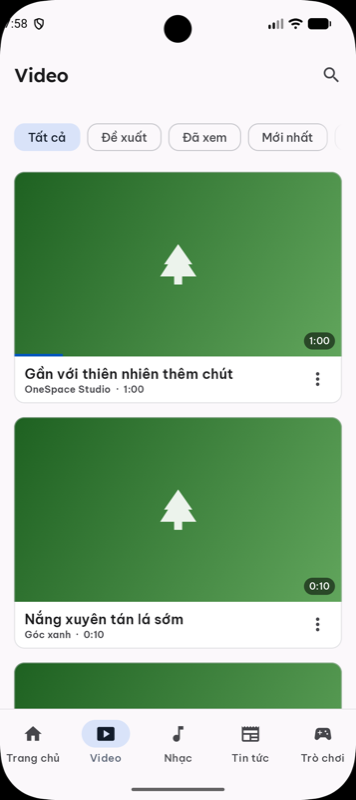
\includegraphics[width=2.75cm]{../figures/app/F-VID-01-01.png}\hspace{0.25cm}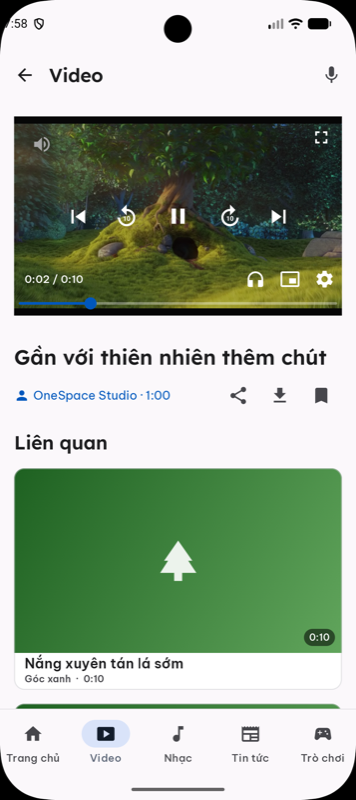
\includegraphics[width=2.75cm]{../figures/app/F-VID-01-02.png}
\end{column}
\end{columns}
\end{frame}

\begin{frame}{Mock Up: Phân hệ Video}
\begin{columns}[T]
\begin{column}{0.46\textwidth}
{\small\bfseries\color{BKTemplate} F-VID-02: Feed ``Đề xuất'' theo sở thích}\\[2.5mm]
Tính năng thuộc nhóm Major Projects
\end{column}
\begin{column}{0.50\textwidth}
\centering
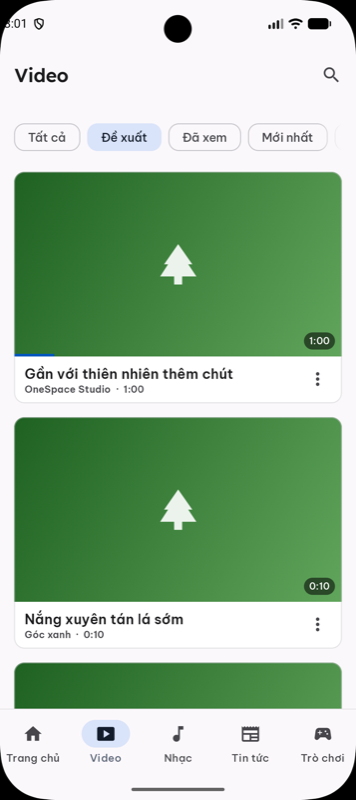
\includegraphics[height=6.1cm]{../figures/app/F-VID-02-01.png}
\end{column}
\end{columns}
\end{frame}

\begin{frame}{Mock Up: Phân hệ Video}
\begin{columns}[T]
\begin{column}{0.46\textwidth}
{\small\bfseries\color{BKTemplate} F-VID-03: Tìm kiếm video}\\[2.5mm]
Tính năng thuộc nhóm Quick Wins
\end{column}
\begin{column}{0.50\textwidth}
\centering
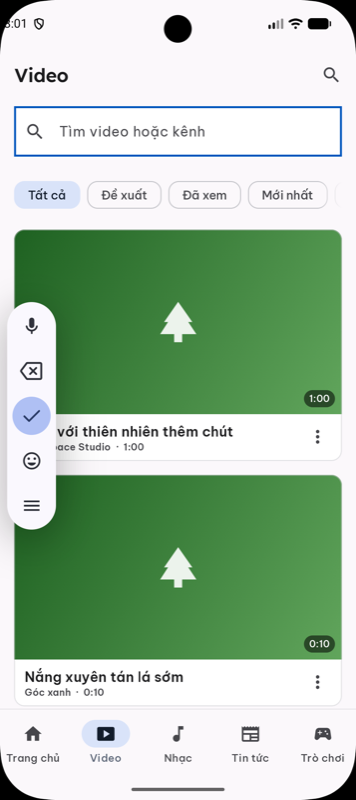
\includegraphics[width=2.75cm]{../figures/app/F-VID-03-01.png}\hspace{0.25cm}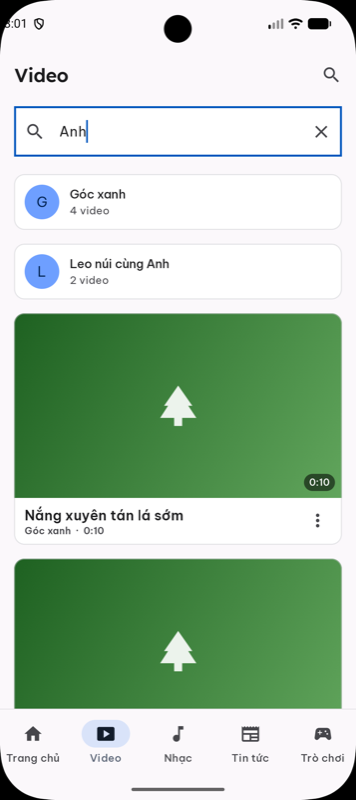
\includegraphics[width=2.75cm]{../figures/app/F-VID-03-02.png}
\end{column}
\end{columns}
\end{frame}

\begin{frame}{Mock Up: Phân hệ Video}
\begin{columns}[T]
\begin{column}{0.46\textwidth}
{\small\bfseries\color{BKTemplate} F-VID-04: Danh sách xem sau (watchlist)}\\[2.5mm]
Tính năng thuộc nhóm Quick Wins
\end{column}
\begin{column}{0.50\textwidth}
\centering
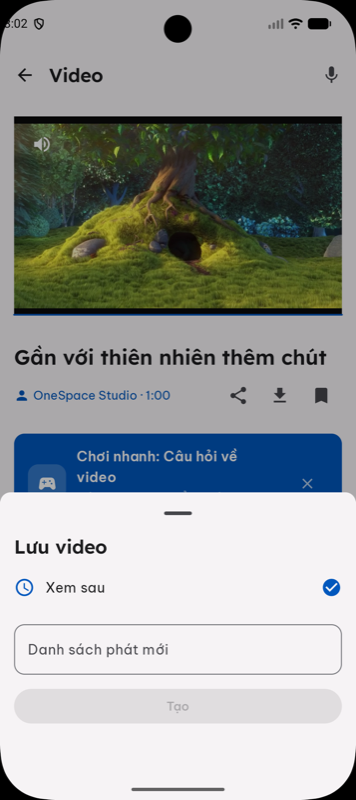
\includegraphics[width=2.75cm]{../figures/app/F-VID-04-01.png}\hspace{0.25cm}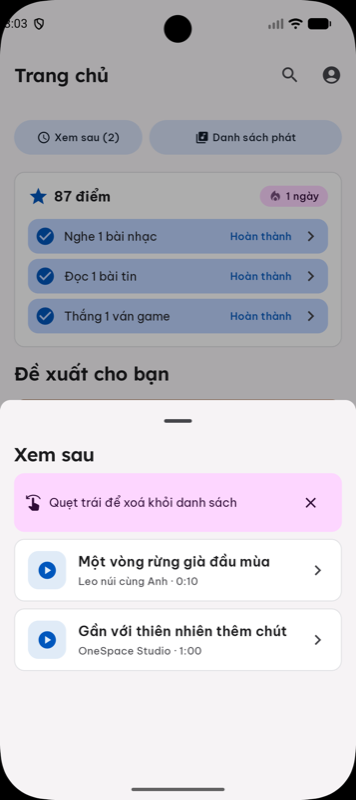
\includegraphics[width=2.75cm]{../figures/app/F-VID-04-02.png}
\end{column}
\end{columns}
\end{frame}

\begin{frame}{Mock Up: Phân hệ Video}
\begin{columns}[T]
\begin{column}{0.46\textwidth}
{\small\bfseries\color{BKTemplate} F-VID-05: Lịch sử xem và tiếp tục từ chỗ dừng}\\[2.5mm]
Tính năng thuộc nhóm Quick Wins
\end{column}
\begin{column}{0.50\textwidth}
\centering
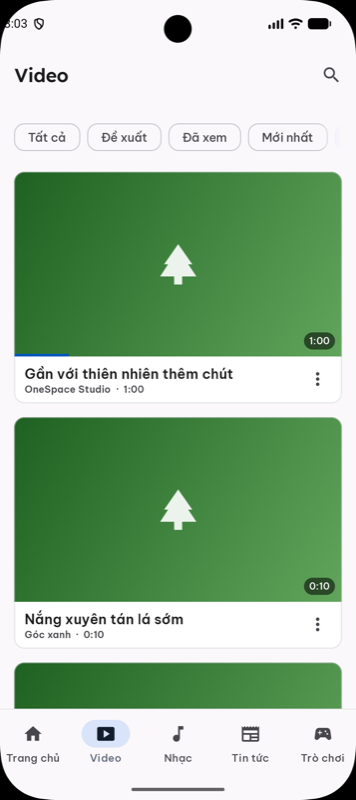
\includegraphics[height=6.1cm]{../figures/app/F-VID-05-01.png}
\end{column}
\end{columns}
\end{frame}

\begin{frame}{Mock Up: Phân hệ Video}
\begin{columns}[T]
\begin{column}{0.46\textwidth}
{\small\bfseries\color{BKTemplate} F-VID-06: Chọn chất lượng phát: Auto hoặc bản 1080p/720p/360p}\\[2.5mm]
Tính năng thuộc nhóm Major Projects
\end{column}
\begin{column}{0.50\textwidth}
\centering
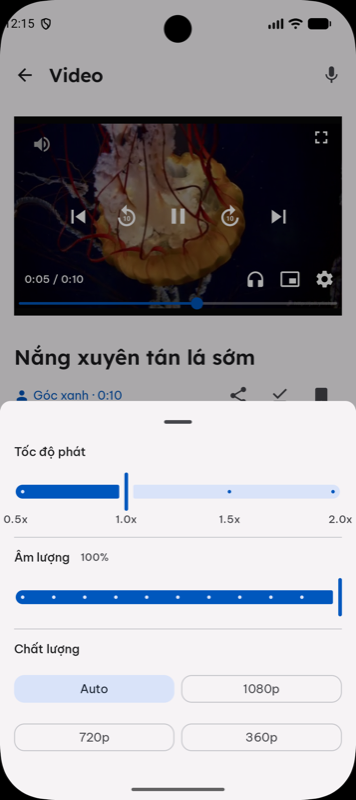
\includegraphics[height=6.1cm]{../figures/app/F-VID-06-01.png}
\end{column}
\end{columns}
\end{frame}

\begin{frame}{Mock Up: Phân hệ Video}
\begin{columns}[T]
\begin{column}{0.46\textwidth}
{\small\bfseries\color{BKTemplate} F-VID-07: Tải video xem offline}\\[2.5mm]
Tính năng thuộc nhóm Thankless
\end{column}
\begin{column}{0.50\textwidth}
\centering
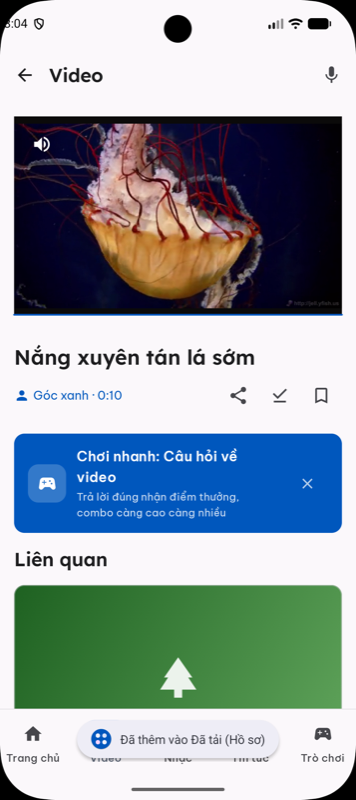
\includegraphics[width=2.32cm]{../figures/app/F-VID-07-01.png}\hspace{0.2cm}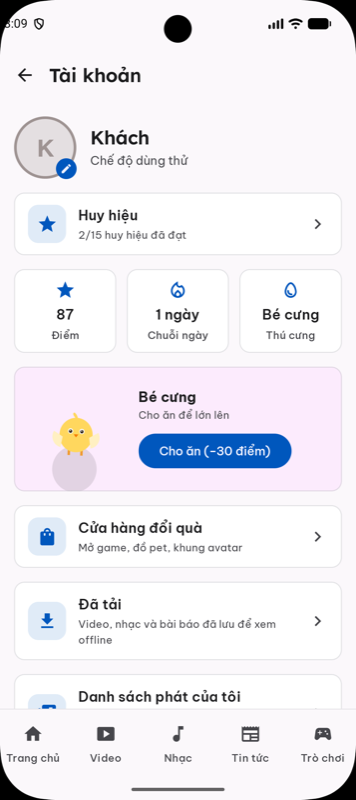
\includegraphics[width=2.32cm]{../figures/app/F-VID-07-02.png}\hspace{0.2cm}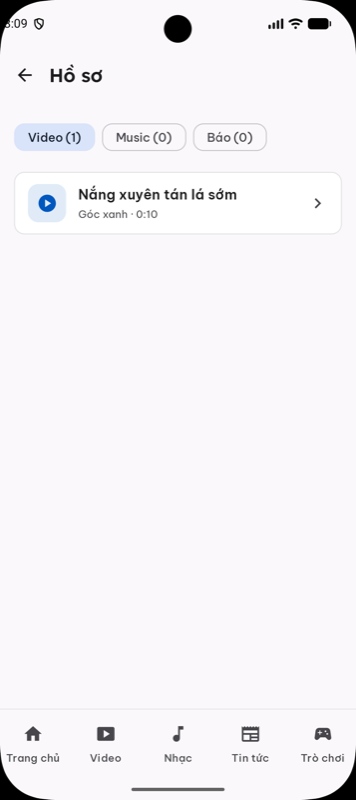
\includegraphics[width=2.32cm]{../figures/app/F-VID-07-03.png}
\end{column}
\end{columns}
\end{frame}

\begin{frame}{Mock Up: Phân hệ Video}
\begin{columns}[T]
\begin{column}{0.46\textwidth}
{\small\bfseries\color{BKTemplate} F-VID-08: Picture-in-picture: video thu nhỏ góc màn hình khi rời trang}\\[2.5mm]
Tính năng thuộc nhóm Major Projects
\end{column}
\begin{column}{0.50\textwidth}
\centering
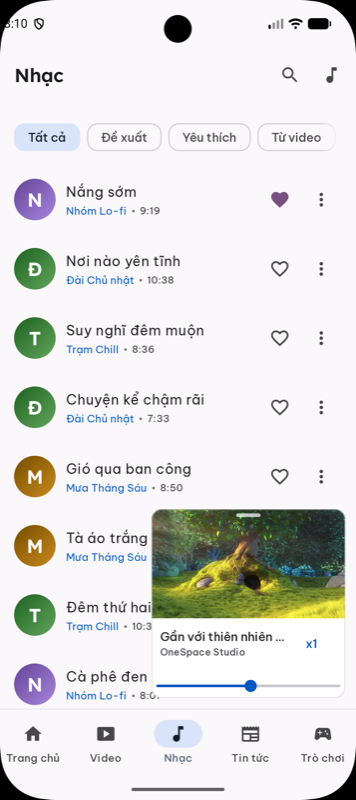
\includegraphics[height=6.1cm]{../figures/app/F-VID-08-01.png}
\end{column}
\end{columns}
\end{frame}

\begin{frame}{Mock Up: Phân hệ Video}
\begin{columns}[T]
\begin{column}{0.46\textwidth}
{\small\bfseries\color{BKTemplate} F-VID-09: Chế độ chỉ phát âm thanh của video (audio-only)}\\[2.5mm]
Tính năng thuộc nhóm Fill-ins
\end{column}
\begin{column}{0.50\textwidth}
\centering
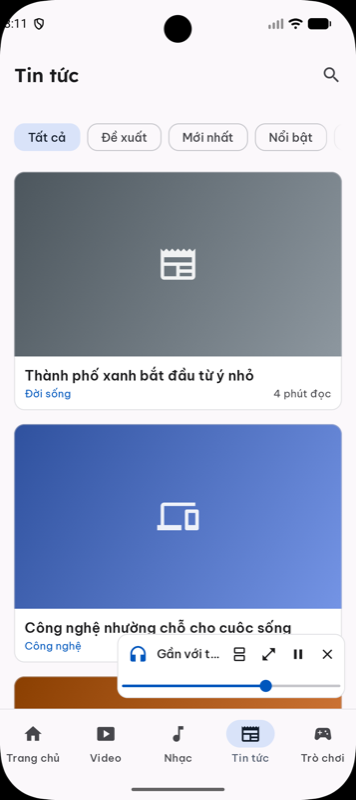
\includegraphics[height=6.1cm]{../figures/app/F-VID-09-01.png}
\end{column}
\end{columns}
\end{frame}

\begin{frame}{Mock Up: Phân hệ Video}
\begin{columns}[T]
\begin{column}{0.46\textwidth}
{\small\bfseries\color{BKTemplate} F-VID-10: Nhấn giữ video để trích thành tệp mp3 cho kho cá nhân}\\[2.5mm]
Tính năng thuộc nhóm Major Projects
\end{column}
\begin{column}{0.50\textwidth}
\centering
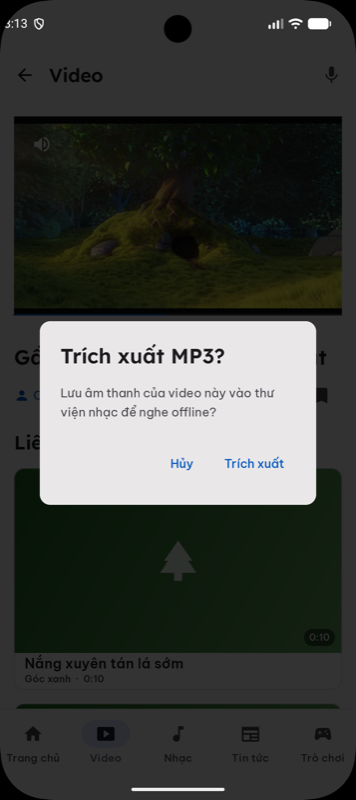
\includegraphics[width=2.32cm]{../figures/app/F-VID-10-01.png}\hspace{0.2cm}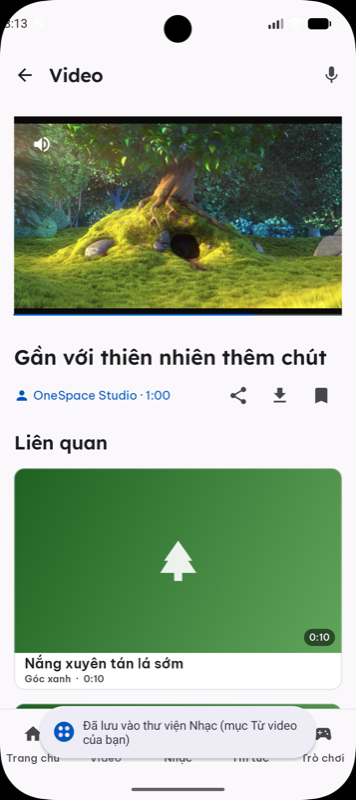
\includegraphics[width=2.32cm]{../figures/app/F-VID-10-02.png}\hspace{0.2cm}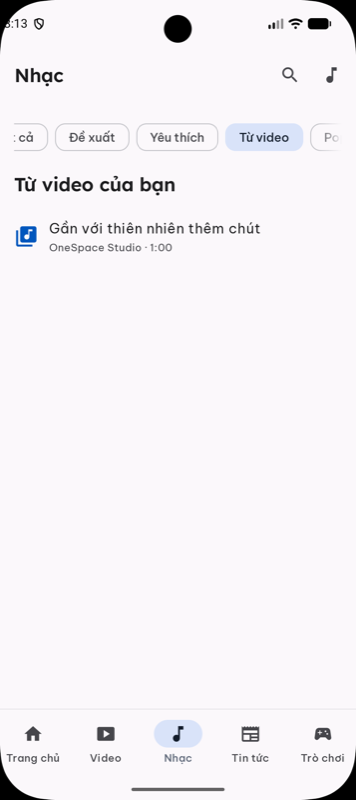
\includegraphics[width=2.32cm]{../figures/app/F-VID-10-03.png}
\end{column}
\end{columns}
\end{frame}

\begin{frame}{Mock Up: Phân hệ Video}
\begin{columns}[T]
\begin{column}{0.46\textwidth}
{\small\bfseries\color{BKTemplate} F-VID-11: Chia sẻ link video ra ngoài app}\\[2.5mm]
Tính năng thuộc nhóm Fill-ins
\end{column}
\begin{column}{0.50\textwidth}
\centering
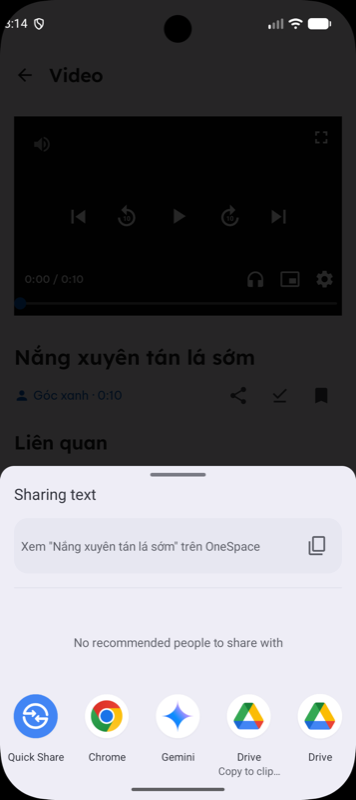
\includegraphics[height=6.1cm]{../figures/app/F-VID-11-01.png}
\end{column}
\end{columns}
\end{frame}

\begin{frame}{Mock Up: Phân hệ Video}
\begin{columns}[T]
\begin{column}{0.46\textwidth}
{\small\bfseries\color{BKTemplate} F-VID-12: Màn hồ sơ nghệ sĩ/kênh: bấm tên để xem mọi nội dung của họ}\\[2.5mm]
Tính năng thuộc nhóm Fill-ins
\end{column}
\begin{column}{0.50\textwidth}
\centering
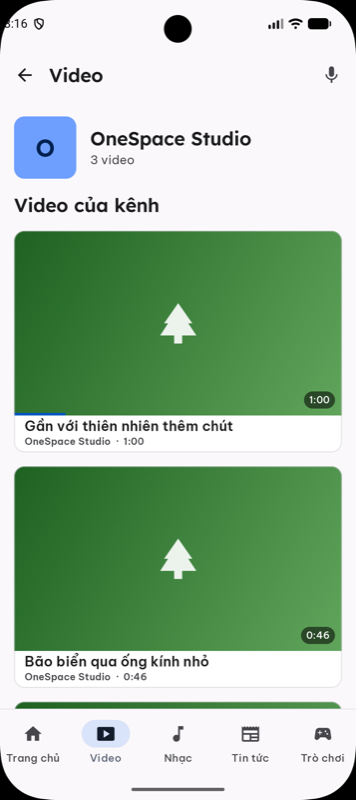
\includegraphics[height=6.1cm]{../figures/app/F-VID-12-01.png}
\end{column}
\end{columns}
\end{frame}

\begin{frame}{Mock Up: Phân hệ Video (1/2)}
\begin{columns}[T]
\begin{column}{0.46\textwidth}
{\small\bfseries\color{BKTemplate} F-VID-13: Playlist video theo chủ đề}\\[2.5mm]
Tính năng thuộc nhóm Fill-ins
\end{column}
\begin{column}{0.50\textwidth}
\centering
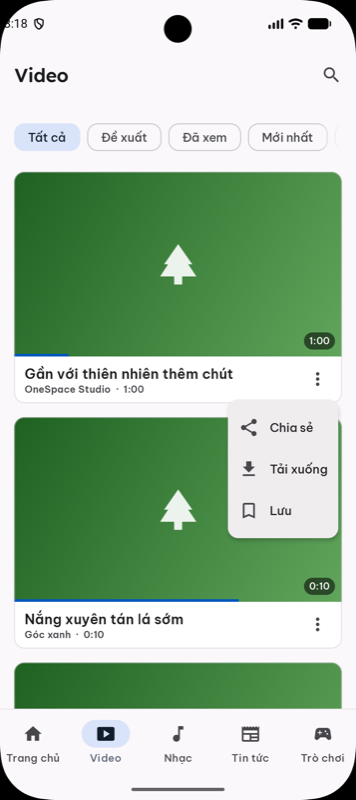
\includegraphics[width=2.75cm]{../figures/app/F-VID-13-01.png}\hspace{0.25cm}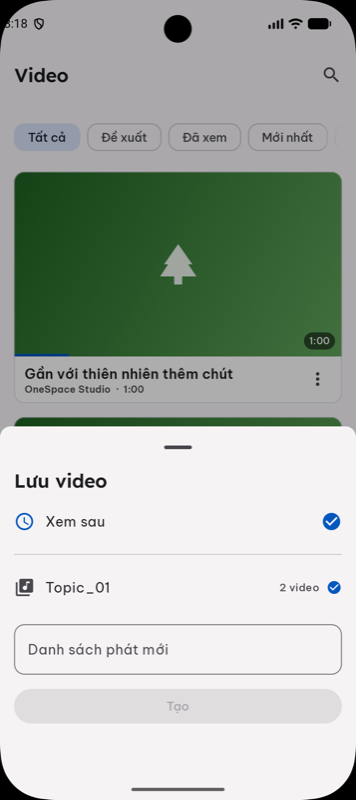
\includegraphics[width=2.75cm]{../figures/app/F-VID-13-02.png}
\end{column}
\end{columns}
\end{frame}

\begin{frame}{Mock Up: Phân hệ Video (2/2)}
\begin{columns}[T]
\begin{column}{0.46\textwidth}
{\small\bfseries\color{BKTemplate} F-VID-13: Playlist video theo chủ đề}\\[2.5mm]
Tính năng thuộc nhóm Fill-ins
\end{column}
\begin{column}{0.50\textwidth}
\centering
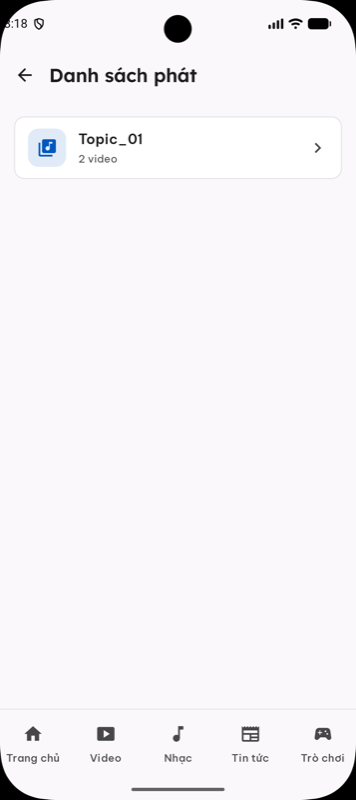
\includegraphics[width=2.75cm]{../figures/app/F-VID-13-03.png}\hspace{0.25cm}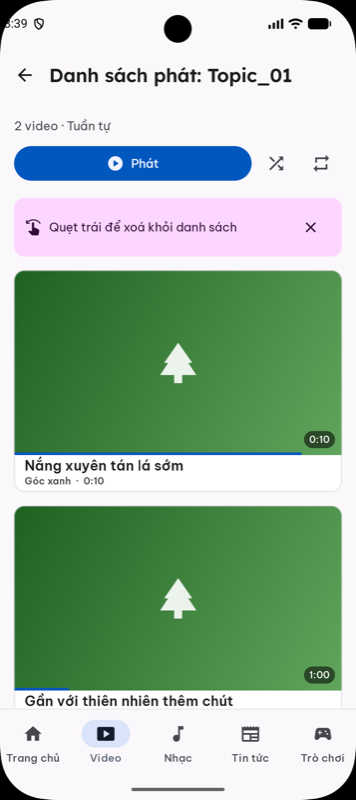
\includegraphics[width=2.75cm]{../figures/app/F-VID-13-04.png}
\end{column}
\end{columns}
\end{frame}

\begin{frame}{Mock Up: Phân hệ Video}
\begin{columns}[T]
\begin{column}{0.46\textwidth}
{\small\bfseries\color{BKTemplate} F-VID-14: Tua nhanh double-tap và đổi tốc độ phát}\\[2.5mm]
Tính năng thuộc nhóm Quick Wins
\end{column}
\begin{column}{0.50\textwidth}
\centering
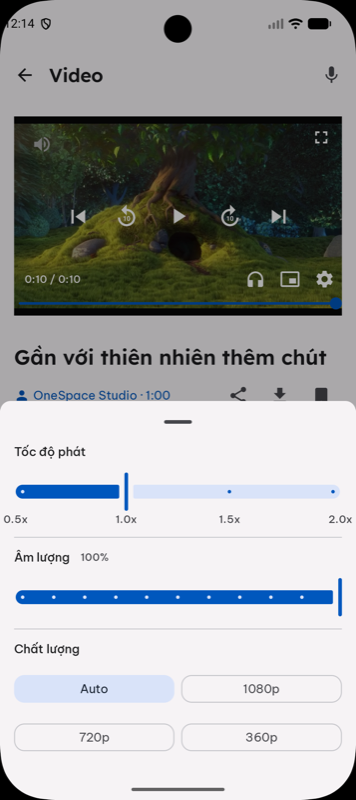
\includegraphics[height=6.1cm]{../figures/app/F-VID-14-01.png}
\end{column}
\end{columns}
\end{frame}

\begin{frame}{Mock Up: Phân hệ Video}
\begin{columns}[T]
\begin{column}{0.46\textwidth}
{\small\bfseries\color{BKTemplate} F-VID-15: Gợi ý ``chơi game liên quan video này'': thẻ game cuối video, câu hỏi soạn sẵn lúc đăng nội dung}\\[2.5mm]
Tính năng thuộc nhóm Quick Wins
\end{column}
\begin{column}{0.50\textwidth}
\centering
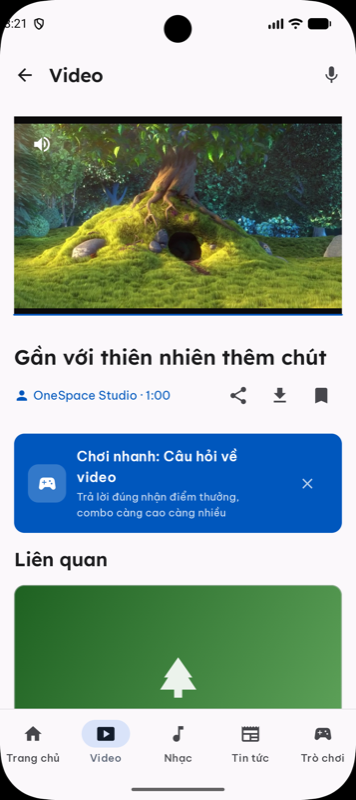
\includegraphics[width=2.75cm]{../figures/app/F-VID-15-01.png}\hspace{0.25cm}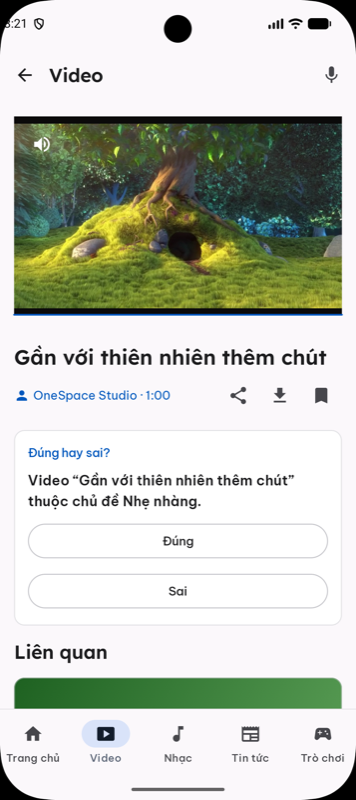
\includegraphics[width=2.75cm]{../figures/app/F-VID-15-02.png}
\end{column}
\end{columns}
\end{frame}

\begin{frame}{Mock Up: Phân hệ Video}
\begin{columns}[T]
\begin{column}{0.46\textwidth}
{\small\bfseries\color{BKTemplate} F-VID-16: Toàn màn hình: nút ẩn system bars, player chiếm cả trang}\\[2.5mm]
Tính năng thuộc nhóm Quick Wins
\end{column}
\begin{column}{0.50\textwidth}
\centering
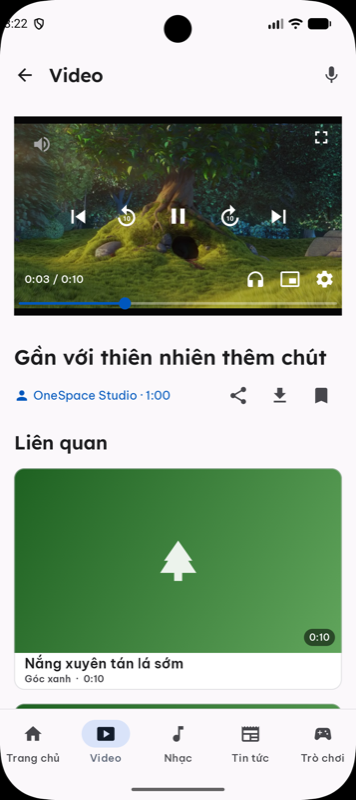
\includegraphics[width=2.75cm]{../figures/app/F-VID-16-01.png}\hspace{0.25cm}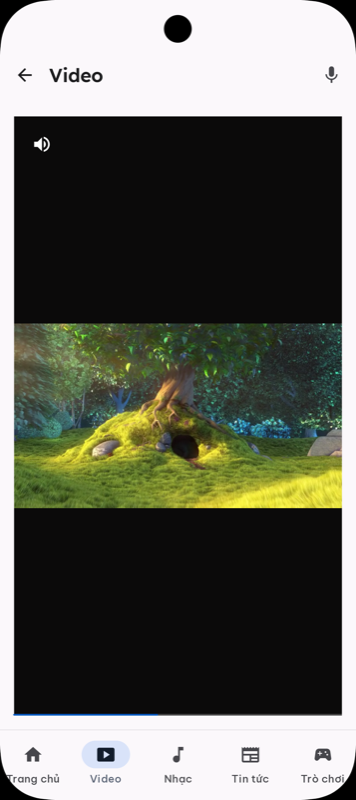
\includegraphics[width=2.75cm]{../figures/app/F-VID-16-02.png}
\end{column}
\end{columns}
\end{frame}

\begin{frame}{Mock Up: Phân hệ Video}
\begin{columns}[T]
\begin{column}{0.46\textwidth}
{\small\bfseries\color{BKTemplate} F-VID-17: Điều khiển âm lượng: nút loa mute/unmute + thanh volume hệ thống}\\[2.5mm]
Tính năng thuộc nhóm Quick Wins
\end{column}
\begin{column}{0.50\textwidth}
\centering
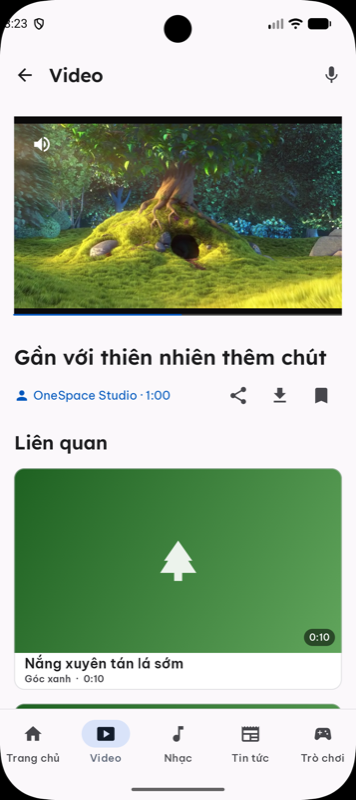
\includegraphics[height=6.1cm]{../figures/app/F-VID-17-01.png}
\end{column}
\end{columns}
\end{frame}

\begin{frame}{Mock Up: Phân hệ Video}
\begin{columns}[T]
\begin{column}{0.46\textwidth}
{\small\bfseries\color{BKTemplate} F-VID-18: Pinch-to-zoom cửa sổ nổi: 2 ngón thu phóng 0.5x--2x}\\[2.5mm]
Tính năng thuộc nhóm Fill-ins
\end{column}
\begin{column}{0.50\textwidth}
\centering
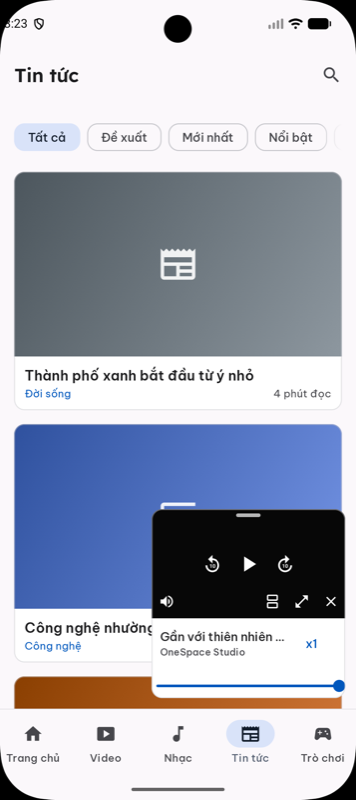
\includegraphics[height=6.1cm]{../figures/app/F-VID-18-01.png}
\end{column}
\end{columns}
\end{frame}

\begin{frame}{Mock Up: Phân hệ Nhạc}
\begin{columns}[T]
\begin{column}{0.46\textwidth}
{\small\bfseries\color{BKTemplate} F-MUS-01: Player nhạc đầy đủ (phát / dừng / chuyển / tua / repeat / shuffle)}\\[2.5mm]
Tính năng thuộc nhóm Major Projects
\end{column}
\begin{column}{0.50\textwidth}
\centering
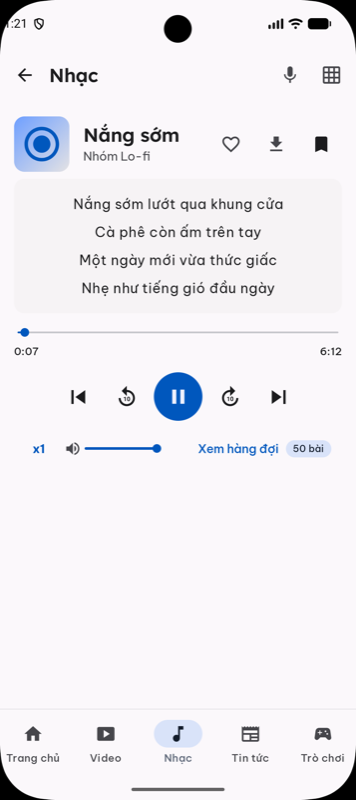
\includegraphics[width=2.75cm]{../figures/app/F-MUS-01-01.png}\hspace{0.25cm}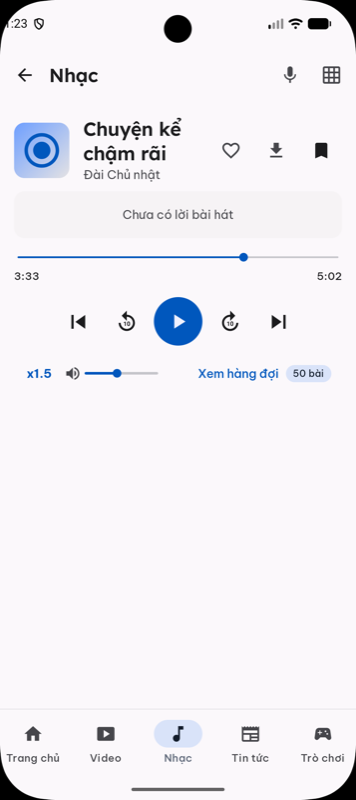
\includegraphics[width=2.75cm]{../figures/app/F-MUS-01-02.png}
\end{column}
\end{columns}
\end{frame}

\begin{frame}{Mock Up: Phân hệ Nhạc}
\begin{columns}[T]
\begin{column}{0.46\textwidth}
{\small\bfseries\color{BKTemplate} F-MUS-02: Mini player dock xuyên suốt mọi màn hình}\\[2.5mm]
Tính năng thuộc nhóm Major Projects
\end{column}
\begin{column}{0.50\textwidth}
\centering
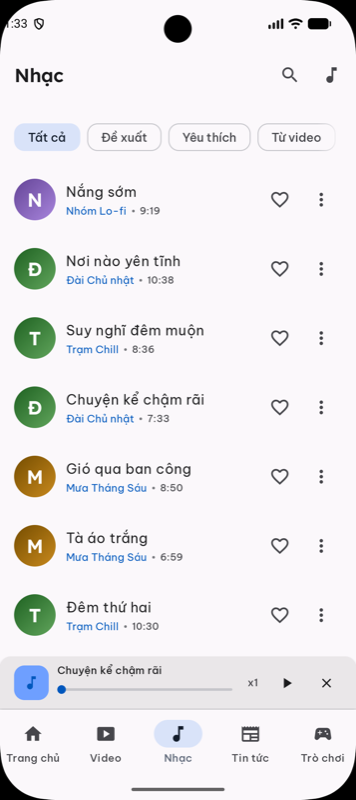
\includegraphics[width=2.75cm]{../figures/app/F-MUS-02-01.png}\hspace{0.25cm}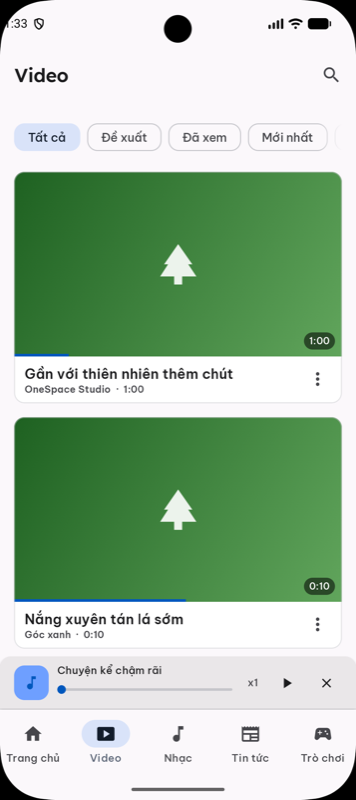
\includegraphics[width=2.75cm]{../figures/app/F-MUS-02-02.png}
\end{column}
\end{columns}
\end{frame}

\begin{frame}{Mock Up: Phân hệ Nhạc}
\begin{columns}[T]
\begin{column}{0.46\textwidth}
{\small\bfseries\color{BKTemplate} F-MUS-03: Phát nhạc nền khi rời ứng dụng hoặc khoá màn hình}\\[2.5mm]
Tính năng thuộc nhóm Major Projects
\end{column}
\begin{column}{0.50\textwidth}
\centering
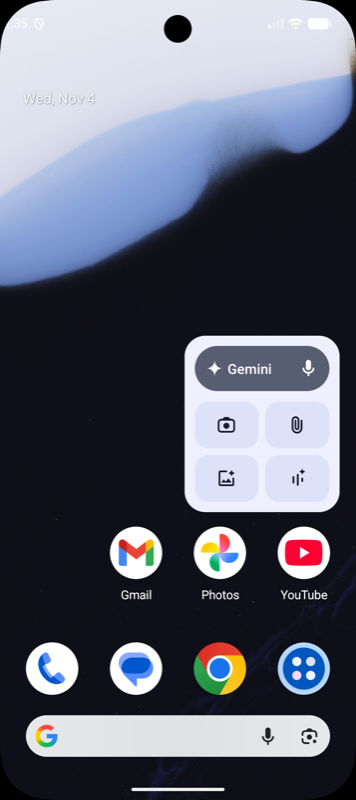
\includegraphics[height=6.1cm]{../figures/app/F-MUS-03-01.png}
\end{column}
\end{columns}
\end{frame}

\begin{frame}{Mock Up: Phân hệ Nhạc}
\begin{columns}[T]
\begin{column}{0.46\textwidth}
{\small\bfseries\color{BKTemplate} F-MUS-04: Tự tạo/sửa/xoá playlist}\\[2.5mm]
Tính năng thuộc nhóm Quick Wins
\end{column}
\begin{column}{0.50\textwidth}
\centering
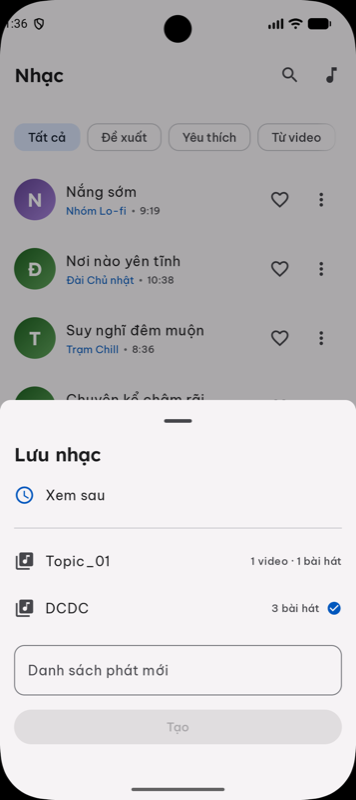
\includegraphics[width=2.75cm]{../figures/app/F-MUS-04-01.png}\hspace{0.25cm}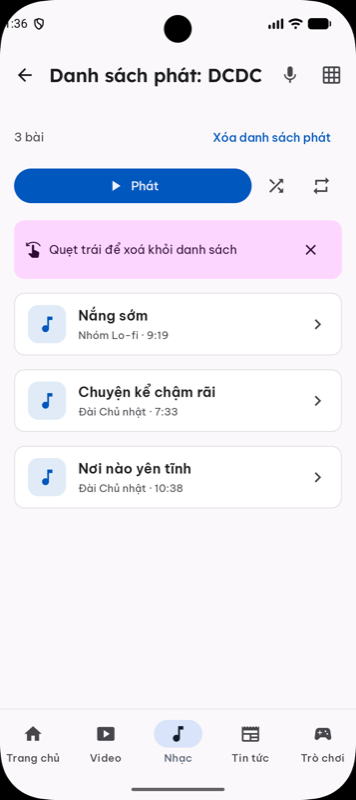
\includegraphics[width=2.75cm]{../figures/app/F-MUS-04-02.png}
\end{column}
\end{columns}
\end{frame}

\begin{frame}{Mock Up: Phân hệ Nhạc}
\begin{columns}[T]
\begin{column}{0.46\textwidth}
{\small\bfseries\color{BKTemplate} F-MUS-05: Hàng phát (queue): thêm tiếp theo, phát cuối, kéo sắp lại}\\[2.5mm]
Tính năng thuộc nhóm Quick Wins
\end{column}
\begin{column}{0.50\textwidth}
\centering
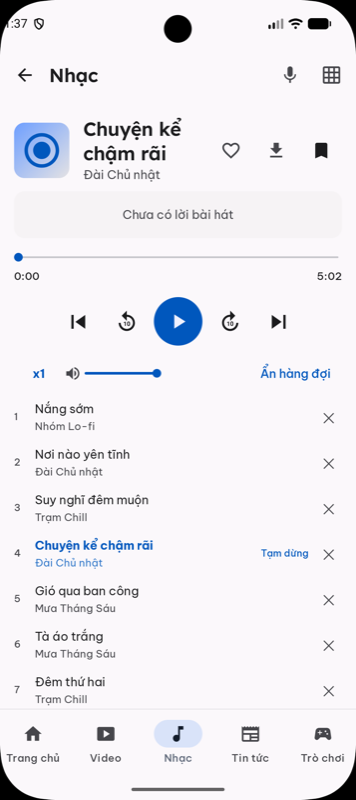
\includegraphics[width=2.75cm]{../figures/app/F-MUS-05-01.png}\hspace{0.25cm}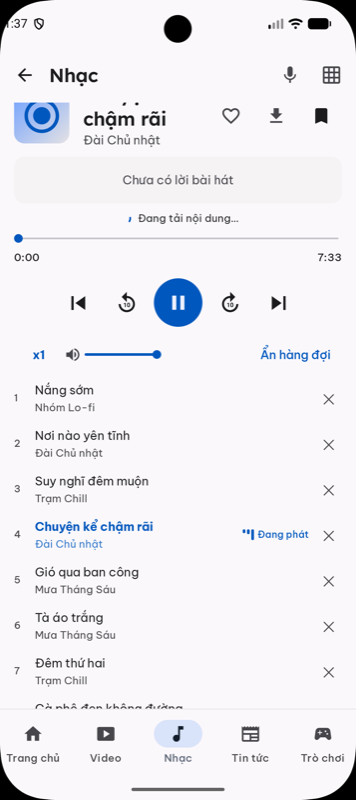
\includegraphics[width=2.75cm]{../figures/app/F-MUS-05-02.png}
\end{column}
\end{columns}
\end{frame}

\begin{frame}{Mock Up: Phân hệ Nhạc}
\begin{columns}[T]
\begin{column}{0.46\textwidth}
{\small\bfseries\color{BKTemplate} F-MUS-06: Tìm kiếm nhạc (bài hát/nghệ sĩ/album)}\\[2.5mm]
Tính năng thuộc nhóm Quick Wins
\end{column}
\begin{column}{0.50\textwidth}
\centering
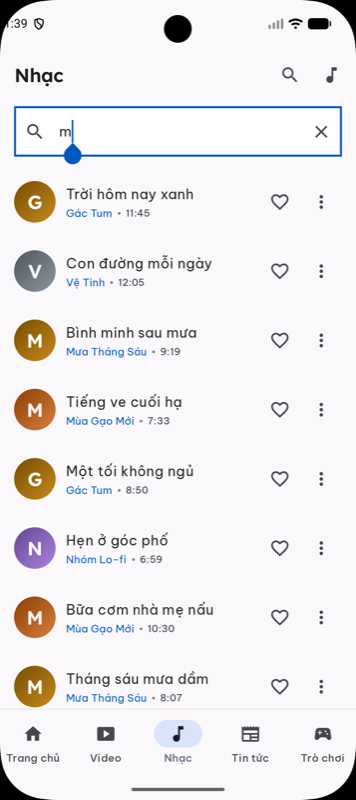
\includegraphics[height=6.1cm]{../figures/app/F-MUS-06-01.png}
\end{column}
\end{columns}
\end{frame}

\begin{frame}{Mock Up: Phân hệ Nhạc}
\begin{columns}[T]
\begin{column}{0.46\textwidth}
{\small\bfseries\color{BKTemplate} F-MUS-07: Kho nhạc cá nhân chứa các tệp trích từ video}\\[2.5mm]
Tính năng thuộc nhóm Major Projects
\end{column}
\begin{column}{0.50\textwidth}
\centering
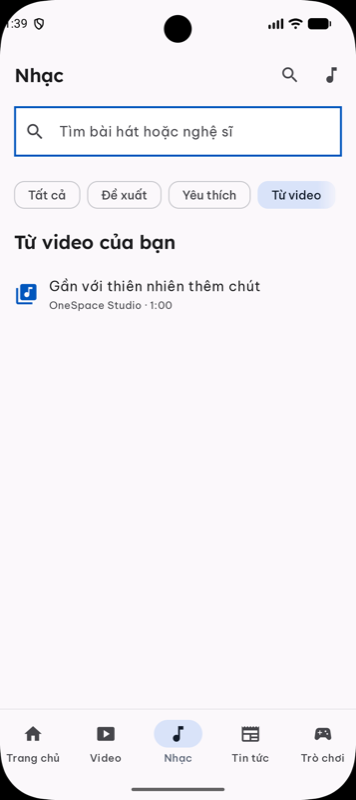
\includegraphics[height=6.1cm]{../figures/app/F-MUS-07-01.png}
\end{column}
\end{columns}
\end{frame}

\begin{frame}{Mock Up: Phân hệ Nhạc}
\begin{columns}[T]
\begin{column}{0.46\textwidth}
{\small\bfseries\color{BKTemplate} F-MUS-08: Gợi ý nhạc theo sở thích}\\[2.5mm]
Tính năng thuộc nhóm Major Projects
\end{column}
\begin{column}{0.50\textwidth}
\centering
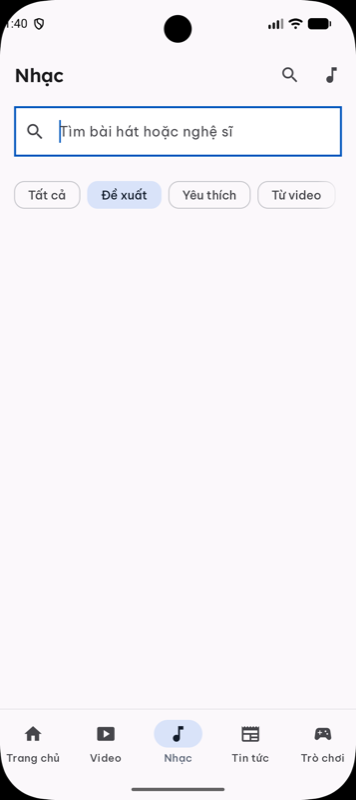
\includegraphics[height=6.1cm]{../figures/app/F-MUS-08-01.png}
\end{column}
\end{columns}
\end{frame}

\begin{frame}{Mock Up: Phân hệ Nhạc}
\begin{columns}[T]
\begin{column}{0.46\textwidth}
{\small\bfseries\color{BKTemplate} F-MUS-09: ``Siêu playlist'' (meta-playlist) trộn nhạc và video}\\[2.5mm]
Tính năng thuộc nhóm Major Projects
\end{column}
\begin{column}{0.50\textwidth}
\centering
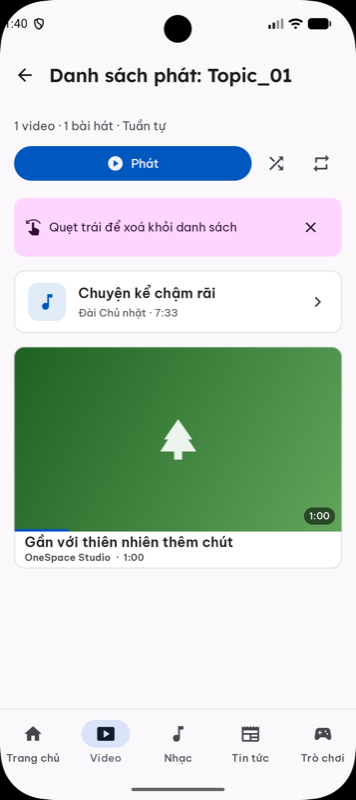
\includegraphics[height=6.1cm]{../figures/app/F-MUS-09-01.png}
\end{column}
\end{columns}
\end{frame}

\begin{frame}{Mock Up: Phân hệ Nhạc}
\begin{columns}[T]
\begin{column}{0.46\textwidth}
{\small\bfseries\color{BKTemplate} F-MUS-10: Xử lý audio focus: duck/pause khi có luồng âm thanh khác}\\[2.5mm]
Tính năng thuộc nhóm Major Projects
\end{column}
\begin{column}{0.50\textwidth}
\centering
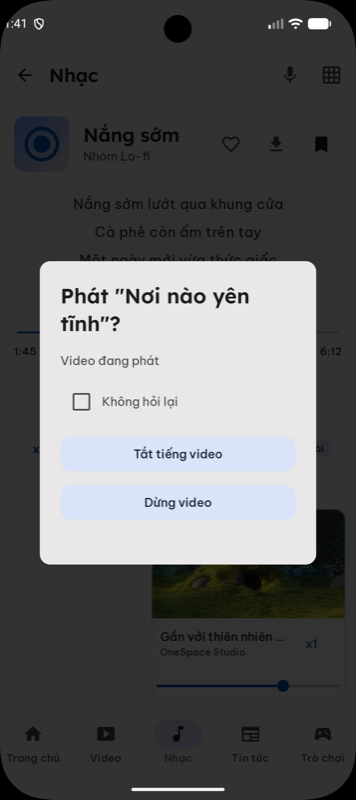
\includegraphics[height=6.1cm]{../figures/app/F-MUS-10-01.png}
\end{column}
\end{columns}
\end{frame}

\begin{frame}{Mock Up: Phân hệ Nhạc}
\begin{columns}[T]
\begin{column}{0.46\textwidth}
{\small\bfseries\color{BKTemplate} F-MUS-12: Tải bài hát offline}\\[2.5mm]
Tính năng thuộc nhóm Thankless
\end{column}
\begin{column}{0.50\textwidth}
\centering
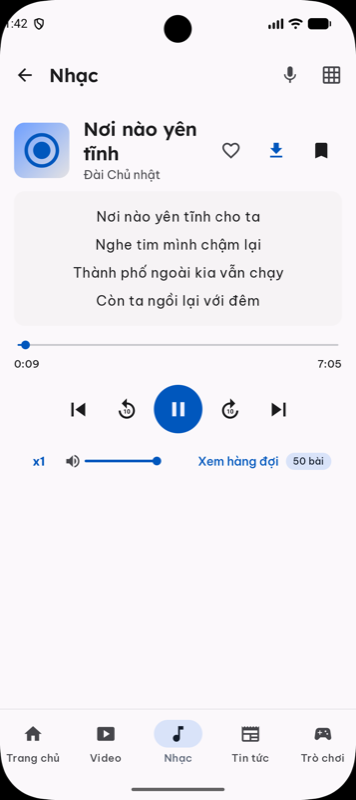
\includegraphics[width=2.75cm]{../figures/app/F-MUS-12-01.png}\hspace{0.25cm}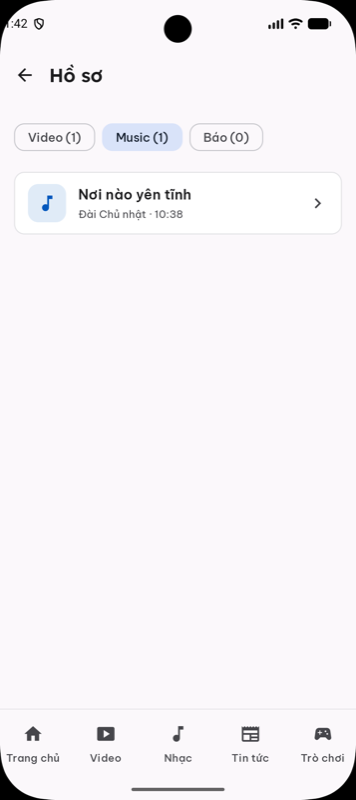
\includegraphics[width=2.75cm]{../figures/app/F-MUS-12-02.png}
\end{column}
\end{columns}
\end{frame}

\begin{frame}{Mock Up: Phân hệ Nhạc}
\begin{columns}[T]
\begin{column}{0.46\textwidth}
{\small\bfseries\color{BKTemplate} F-MUS-13: Tốc độ phát nhạc: x1/x1.5/x2/x0.5 trên dock và Home card}\\[2.5mm]
Tính năng thuộc nhóm Quick Wins
\end{column}
\begin{column}{0.50\textwidth}
\centering
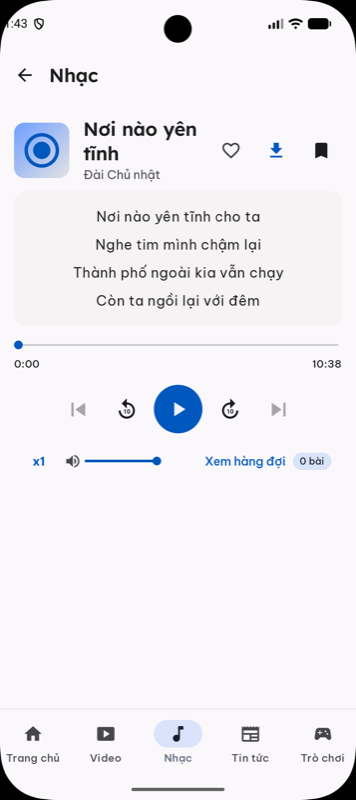
\includegraphics[width=2.75cm]{../figures/app/F-MUS-13-01.png}\hspace{0.25cm}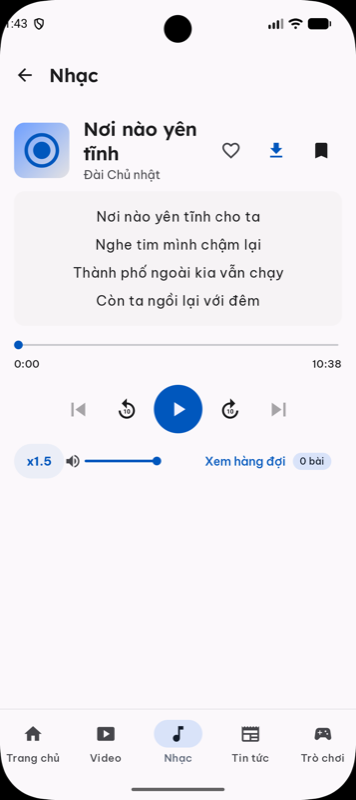
\includegraphics[width=2.75cm]{../figures/app/F-MUS-13-02.png}
\end{column}
\end{columns}
\end{frame}

\begin{frame}{Mock Up: Phân hệ Nhạc}
\begin{columns}[T]
\begin{column}{0.46\textwidth}
{\small\bfseries\color{BKTemplate} F-MUS-14: Lời bài hát: panel scroll trên Now Playing}\\[2.5mm]
Tính năng thuộc nhóm Fill-ins
\end{column}
\begin{column}{0.50\textwidth}
\centering
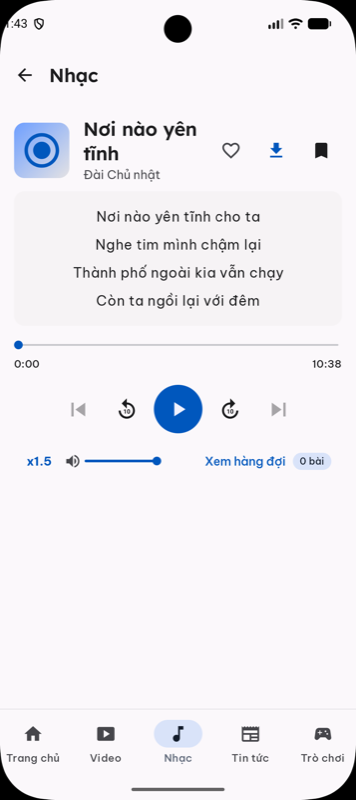
\includegraphics[height=6.1cm]{../figures/app/F-MUS-14-01.png}
\end{column}
\end{columns}
\end{frame}

\begin{frame}{Mock Up: Phân hệ Tin tức}
\begin{columns}[T]
\begin{column}{0.46\textwidth}
{\small\bfseries\color{BKTemplate} F-NEWS-01: Feed tin theo chuyên mục và sở thích}\\[2.5mm]
Tính năng thuộc nhóm Major Projects
\end{column}
\begin{column}{0.50\textwidth}
\centering
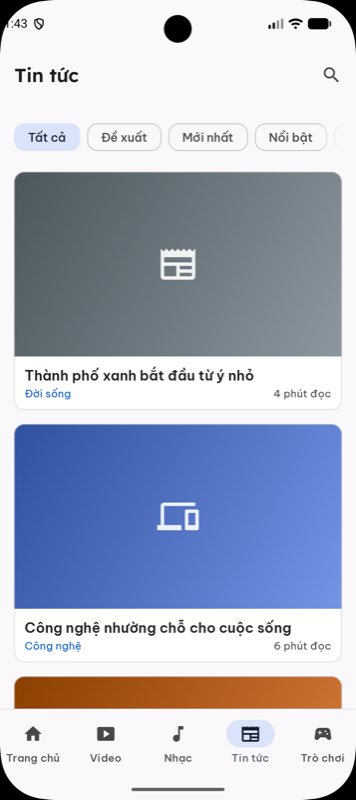
\includegraphics[width=2.75cm]{../figures/app/F-NEWS-01-01.png}\hspace{0.25cm}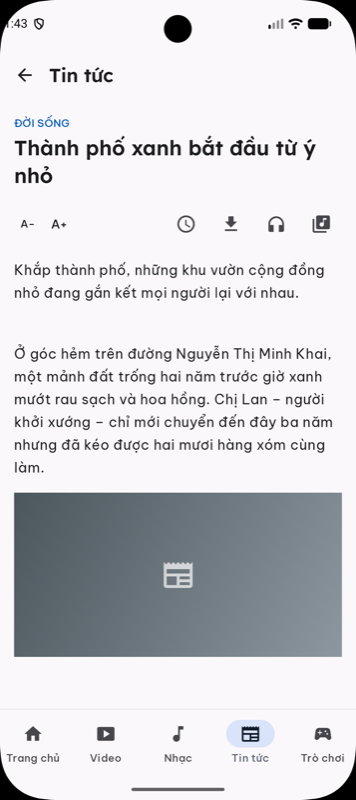
\includegraphics[width=2.75cm]{../figures/app/F-NEWS-01-02.png}
\end{column}
\end{columns}
\end{frame}

\begin{frame}{Mock Up: Phân hệ Tin tức}
\begin{columns}[T]
\begin{column}{0.46\textwidth}
{\small\bfseries\color{BKTemplate} F-NEWS-02: Trình đọc sạch, đổi cỡ chữ}\\[2.5mm]
Tính năng thuộc nhóm Quick Wins
\end{column}
\begin{column}{0.50\textwidth}
\centering

\includegraphics[height=6.1cm]{../figures/app/F-NEWS-02-01.png}
\end{column}
\end{columns}
\end{frame}

\begin{frame}{Mock Up: Phân hệ Tin tức}
\begin{columns}[T]
\begin{column}{0.46\textwidth}
{\small\bfseries\color{BKTemplate} F-NEWS-03: Lưu bài đọc sau}\\[2.5mm]
Tính năng thuộc nhóm Quick Wins
\end{column}
\begin{column}{0.50\textwidth}
\centering

\includegraphics[height=6.1cm]{../figures/app/F-NEWS-03-01.png}
\end{column}
\end{columns}
\end{frame}

\begin{frame}{Mock Up: Phân hệ Tin tức}
\begin{columns}[T]
\begin{column}{0.46\textwidth}
{\small\bfseries\color{BKTemplate} F-NEWS-04: Tìm kiếm bài báo}\\[2.5mm]
Tính năng thuộc nhóm Fill-ins
\end{column}
\begin{column}{0.50\textwidth}
\centering
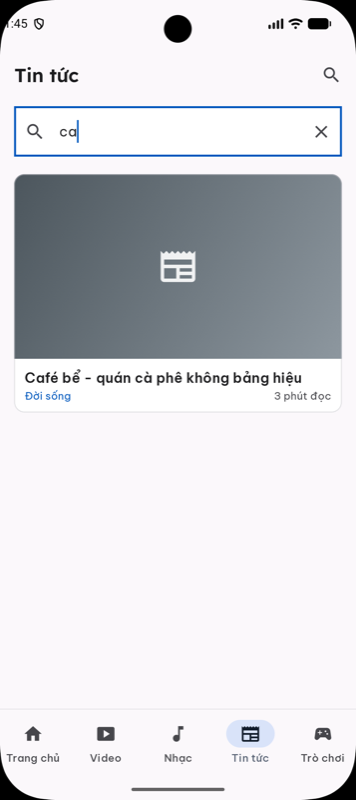
\includegraphics[height=6.1cm]{../figures/app/F-NEWS-04-01.png}
\end{column}
\end{columns}
\end{frame}

\begin{frame}{Mock Up: Phân hệ Tin tức}
\begin{columns}[T]
\begin{column}{0.46\textwidth}
{\small\bfseries\color{BKTemplate} F-NEWS-05: Chuyển bài báo thành audio (TTS)~--~``nghe tin''}\\[2.5mm]
Tính năng thuộc nhóm Major Projects
\end{column}
\begin{column}{0.50\textwidth}
\centering
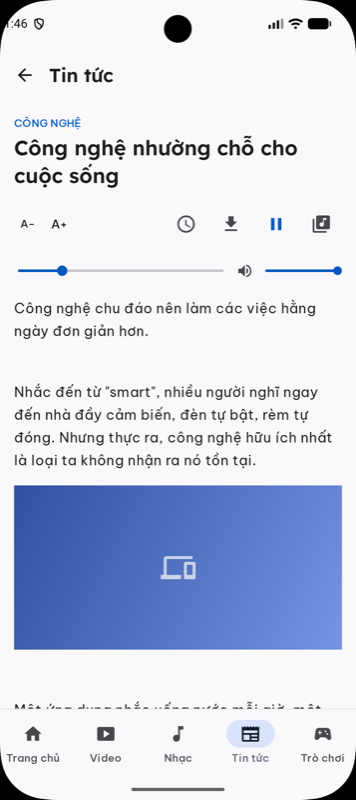
\includegraphics[width=2.75cm]{../figures/app/F-NEWS-05-01.png}\hspace{0.25cm}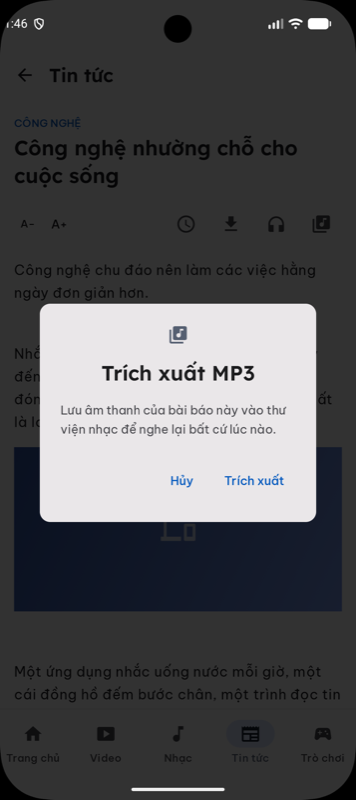
\includegraphics[width=2.75cm]{../figures/app/F-NEWS-05-02.png}
\end{column}
\end{columns}
\end{frame}

\begin{frame}{Mock Up: Phân hệ Tin tức}
\begin{columns}[T]
\begin{column}{0.46\textwidth}
{\small\bfseries\color{BKTemplate} F-NEWS-06: Sắp xếp mới nhất / phổ biến}\\[2.5mm]
Tính năng thuộc nhóm Quick Wins
\end{column}
\begin{column}{0.50\textwidth}
\centering
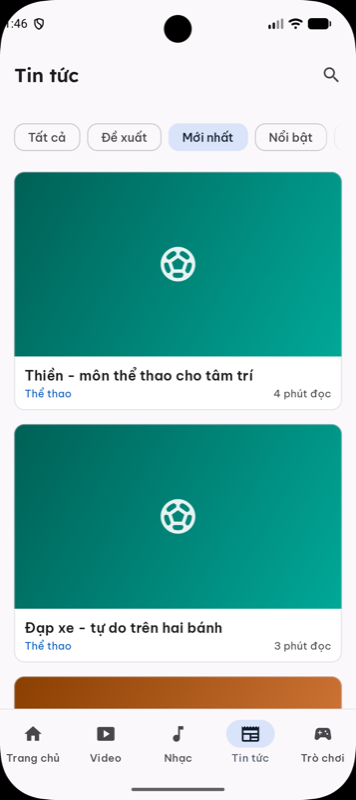
\includegraphics[height=6.1cm]{../figures/app/F-NEWS-06-01.png}
\end{column}
\end{columns}
\end{frame}

\begin{frame}{Mock Up: Phân hệ Tin tức}
\begin{columns}[T]
\begin{column}{0.46\textwidth}
{\small\bfseries\color{BKTemplate} F-NEWS-07: Nghe nhạc khi đọc tin (dock vẫn phát)}\\[2.5mm]
Tính năng thuộc nhóm Quick Wins
\end{column}
\begin{column}{0.50\textwidth}
\centering
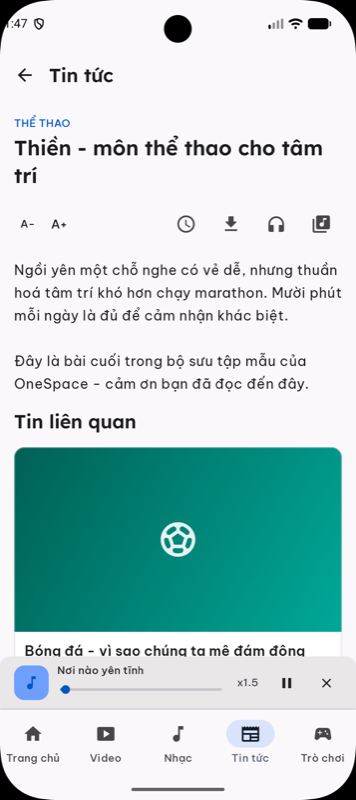
\includegraphics[height=6.1cm]{../figures/app/F-NEWS-07-01.png}
\end{column}
\end{columns}
\end{frame}

\begin{frame}{Mock Up: Phân hệ Tin tức}
\begin{columns}[T]
\begin{column}{0.46\textwidth}
{\small\bfseries\color{BKTemplate} F-NEWS-08: Quiz sinh ra từ bài báo đang đọc}\\[2.5mm]
Tính năng thuộc nhóm Major Projects
\end{column}
\begin{column}{0.50\textwidth}
\centering
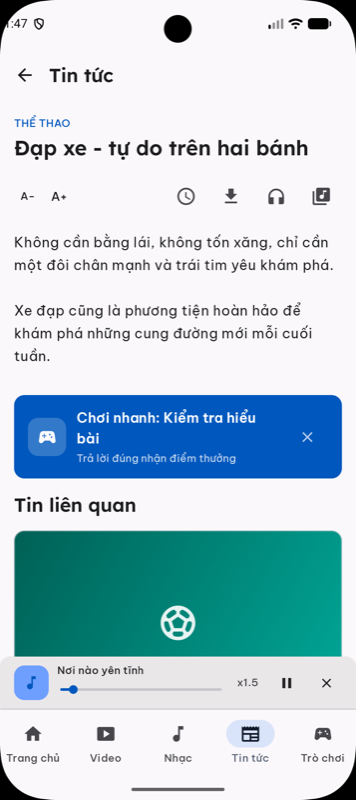
\includegraphics[width=2.75cm]{../figures/app/F-NEWS-08-01.png}\hspace{0.25cm}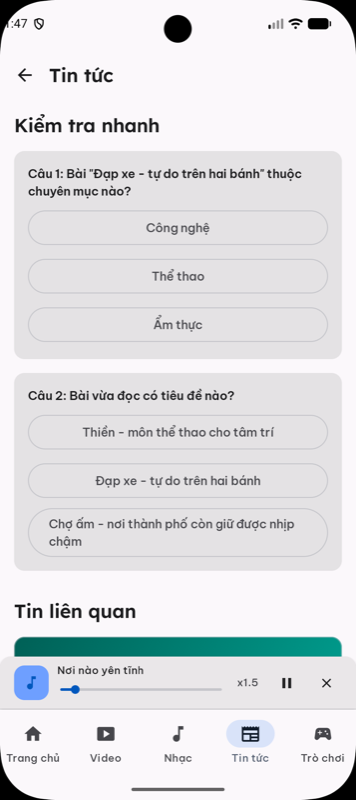
\includegraphics[width=2.75cm]{../figures/app/F-NEWS-08-02.png}
\end{column}
\end{columns}
\end{frame}

\begin{frame}{Mock Up: Phân hệ Tin tức}
\begin{columns}[T]
\begin{column}{0.46\textwidth}
{\small\bfseries\color{BKTemplate} F-NEWS-09: Gợi ý bài liên quan}\\[2.5mm]
Tính năng thuộc nhóm Fill-ins
\end{column}
\begin{column}{0.50\textwidth}
\centering
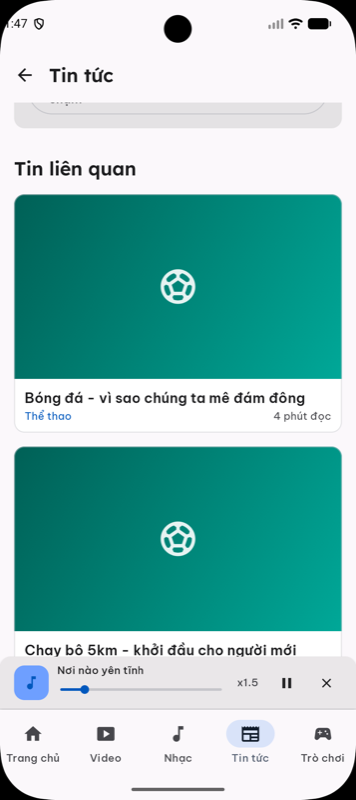
\includegraphics[height=6.1cm]{../figures/app/F-NEWS-09-01.png}
\end{column}
\end{columns}
\end{frame}

\begin{frame}{Mock Up: Phân hệ Tin tức}
\begin{columns}[T]
\begin{column}{0.46\textwidth}
{\small\bfseries\color{BKTemplate} F-NEWS-10: Bài đang đọc thu nhỏ thành thẻ nổi khi rời tab News}\\[2.5mm]
Tính năng thuộc nhóm Major Projects
\end{column}
\begin{column}{0.50\textwidth}
\centering
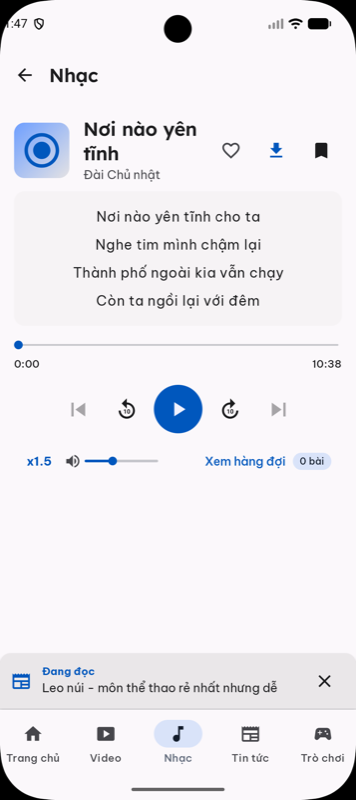
\includegraphics[width=2.75cm]{../figures/app/F-NEWS-10-01.png}\hspace{0.25cm}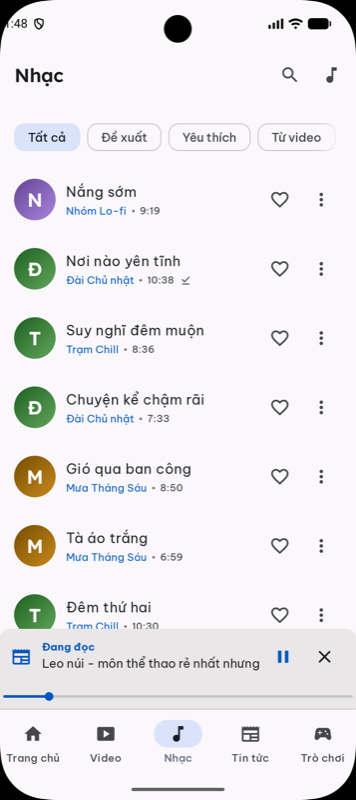
\includegraphics[width=2.75cm]{../figures/app/F-NEWS-10-02.png}
\end{column}
\end{columns}
\end{frame}

\begin{frame}{Mock Up: Phân hệ Trò chơi}
\begin{columns}[T]
\begin{column}{0.46\textwidth}
{\small\bfseries\color{BKTemplate} F-GAME-01: Hub minigame: danh sách, trạng thái mở khoá, phần thưởng}\\[2.5mm]
Tính năng thuộc nhóm Quick Wins
\end{column}
\begin{column}{0.50\textwidth}
\centering
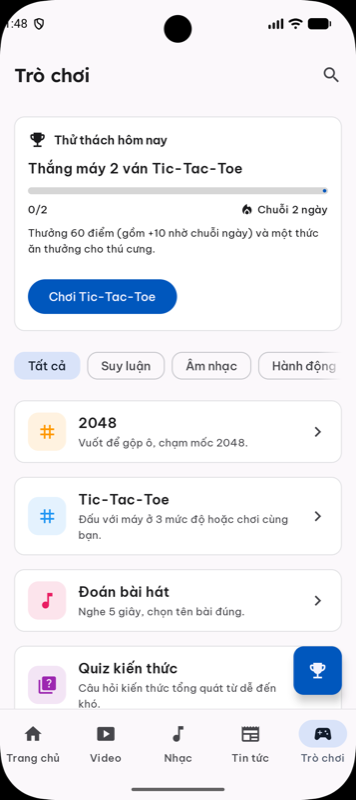
\includegraphics[height=6.1cm]{../figures/app/F-GAME-01-01.png}
\end{column}
\end{columns}
\end{frame}

\begin{frame}{Mock Up: Phân hệ Trò chơi}
\begin{columns}[T]
\begin{column}{0.46\textwidth}
{\small\bfseries\color{BKTemplate} F-GAME-02: Game đoán bài hát}\\[2.5mm]
Tính năng thuộc nhóm Major Projects
\end{column}
\begin{column}{0.50\textwidth}
\centering
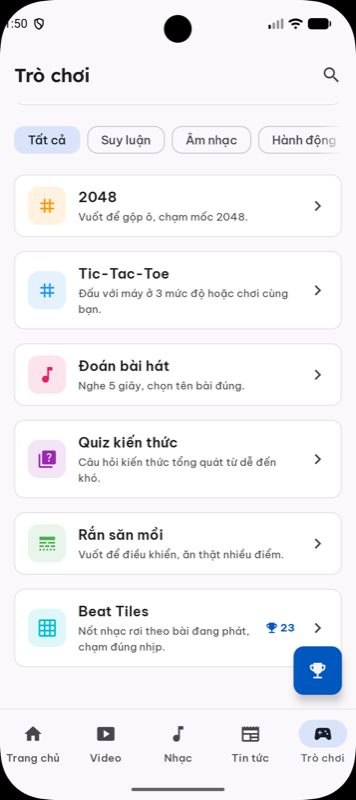
\includegraphics[width=2.32cm]{../figures/app/F-GAME-02-01.png}\hspace{0.2cm}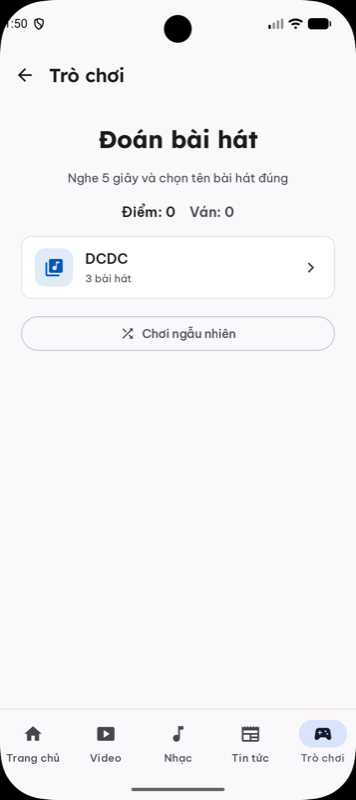
\includegraphics[width=2.32cm]{../figures/app/F-GAME-02-02.png}\hspace{0.2cm}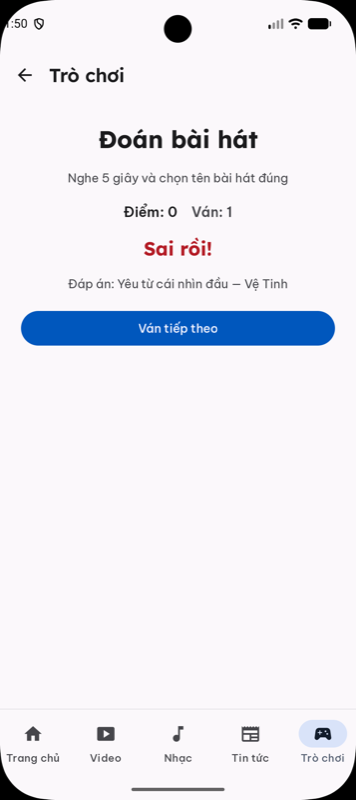
\includegraphics[width=2.32cm]{../figures/app/F-GAME-02-03.png}
\end{column}
\end{columns}
\end{frame}

\begin{frame}{Mock Up: Phân hệ Trò chơi}
\begin{columns}[T]
\begin{column}{0.46\textwidth}
{\small\bfseries\color{BKTemplate} F-GAME-03: Quiz tin tức}\\[2.5mm]
Tính năng thuộc nhóm Major Projects
\end{column}
\begin{column}{0.50\textwidth}
\centering
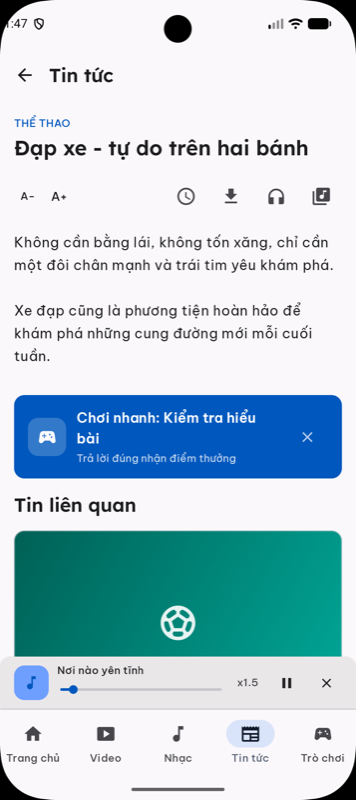
\includegraphics[width=2.75cm]{../figures/app/F-GAME-03-01.png}\hspace{0.25cm}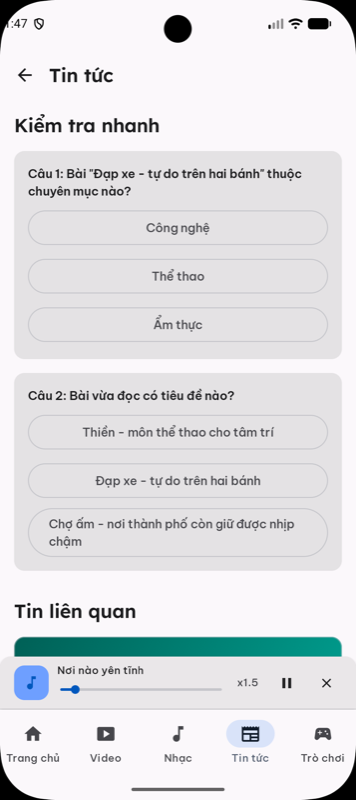
\includegraphics[width=2.75cm]{../figures/app/F-GAME-03-02.png}
\end{column}
\end{columns}
\end{frame}

\begin{frame}{Mock Up: Phân hệ Trò chơi}
\begin{columns}[T]
\begin{column}{0.46\textwidth}
{\small\bfseries\color{BKTemplate} F-GAME-04: Quiz kiến thức (kiểu Ai là triệu phú)}\\[2.5mm]
Tính năng thuộc nhóm Fill-ins
\end{column}
\begin{column}{0.50\textwidth}
\centering
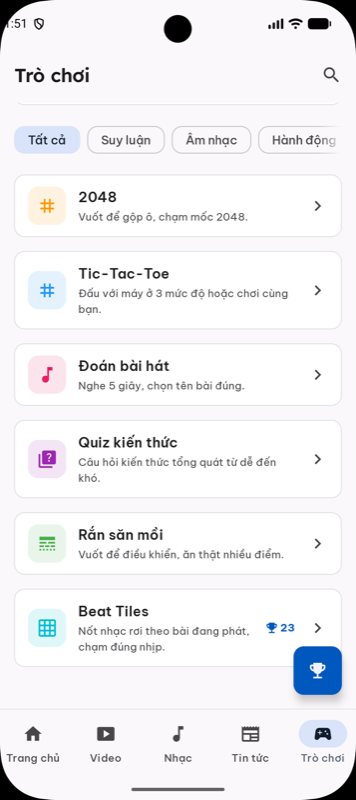
\includegraphics[width=2.32cm]{../figures/app/F-GAME-04-01.png}\hspace{0.2cm}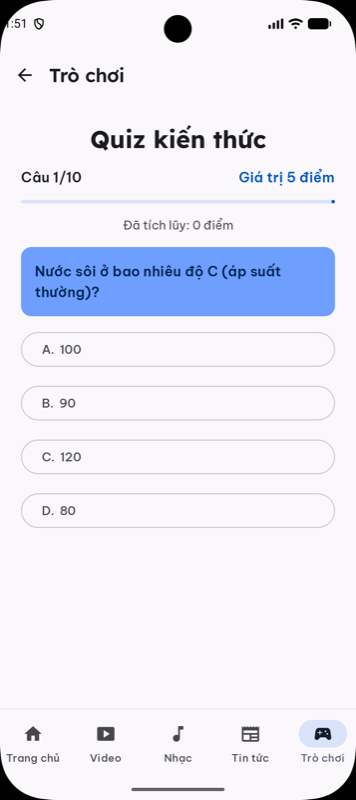
\includegraphics[width=2.32cm]{../figures/app/F-GAME-04-02.png}\hspace{0.2cm}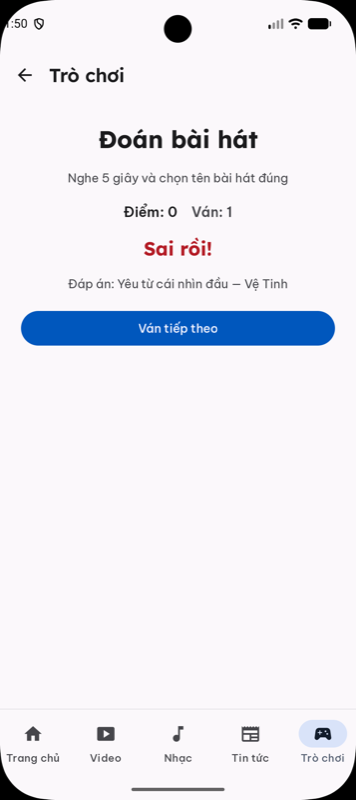
\includegraphics[width=2.32cm]{../figures/app/F-GAME-04-03.png}
\end{column}
\end{columns}
\end{frame}

\begin{frame}{Mock Up: Phân hệ Trò chơi}
\begin{columns}[T]
\begin{column}{0.46\textwidth}
{\small\bfseries\color{BKTemplate} F-GAME-05: Snake -- rắn săn mồi}\\[2.5mm]
Tính năng thuộc nhóm Fill-ins
\end{column}
\begin{column}{0.50\textwidth}
\centering
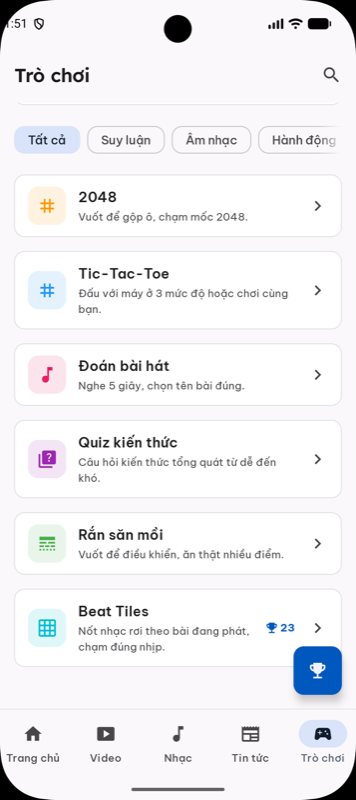
\includegraphics[width=2.32cm]{../figures/app/F-GAME-05-01.png}\hspace{0.2cm}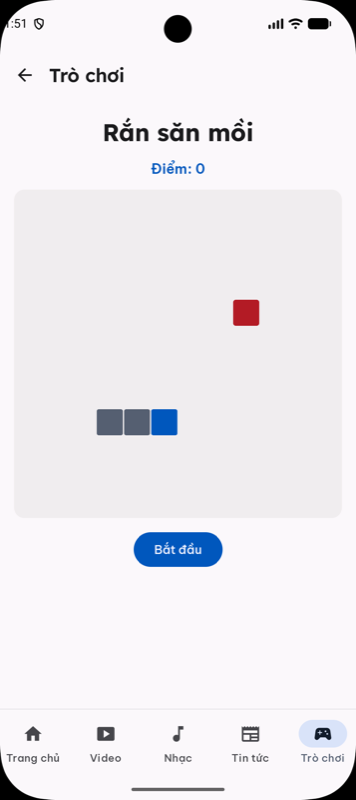
\includegraphics[width=2.32cm]{../figures/app/F-GAME-05-02.png}\hspace{0.2cm}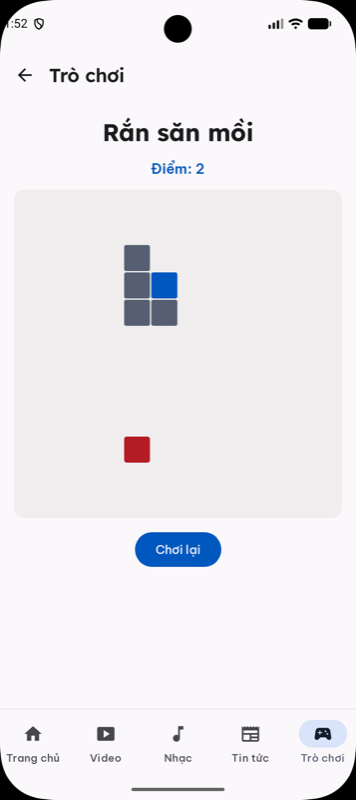
\includegraphics[width=2.32cm]{../figures/app/F-GAME-05-03.png}
\end{column}
\end{columns}
\end{frame}

\begin{frame}{Mock Up: Phân hệ Trò chơi (1/2)}
\begin{columns}[T]
\begin{column}{0.46\textwidth}
{\small\bfseries\color{BKTemplate} F-GAME-06: ``Beat tiles'' -- nốt nhạc rơi theo bài đang phát (kiểu piano tiles)}\\[2.5mm]
Tính năng thuộc nhóm Quick Wins
\end{column}
\begin{column}{0.50\textwidth}
\centering
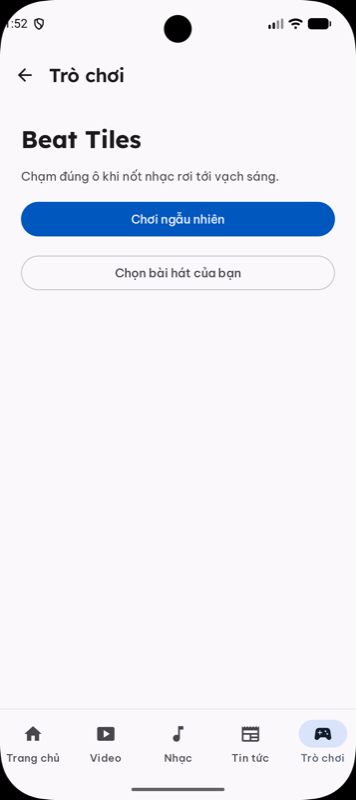
\includegraphics[width=2.75cm]{../figures/app/F-GAME-06-01.png}\hspace{0.25cm}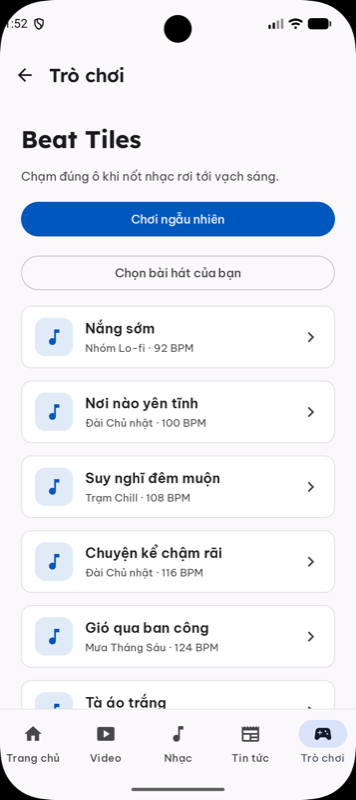
\includegraphics[width=2.75cm]{../figures/app/F-GAME-06-02.png}
\end{column}
\end{columns}
\end{frame}

\begin{frame}{Mock Up: Phân hệ Trò chơi (2/2)}
\begin{columns}[T]
\begin{column}{0.46\textwidth}
{\small\bfseries\color{BKTemplate} F-GAME-06: ``Beat tiles'' -- nốt nhạc rơi theo bài đang phát (kiểu piano tiles)}\\[2.5mm]
Tính năng thuộc nhóm Quick Wins
\end{column}
\begin{column}{0.50\textwidth}
\centering
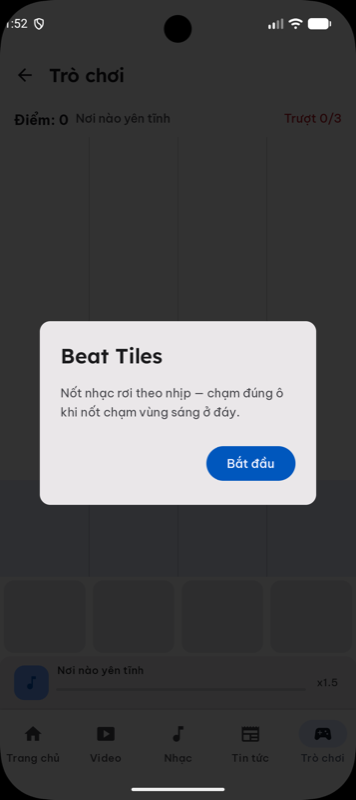
\includegraphics[width=2.75cm]{../figures/app/F-GAME-06-03.png}\hspace{0.25cm}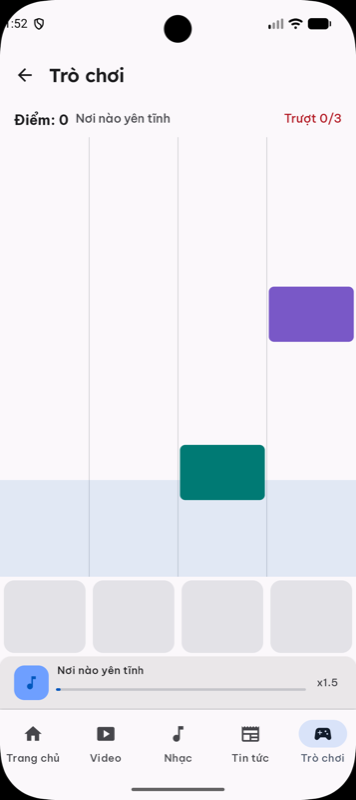
\includegraphics[width=2.75cm]{../figures/app/F-GAME-06-04.png}
\end{column}
\end{columns}
\end{frame}

\begin{frame}{Mock Up: Phân hệ Trò chơi}
\begin{columns}[T]
\begin{column}{0.46\textwidth}
{\small\bfseries\color{BKTemplate} F-GAME-07: Bảng xếp hạng tuần/tháng}\\[2.5mm]
Tính năng thuộc nhóm Major Projects
\end{column}
\begin{column}{0.50\textwidth}
\centering
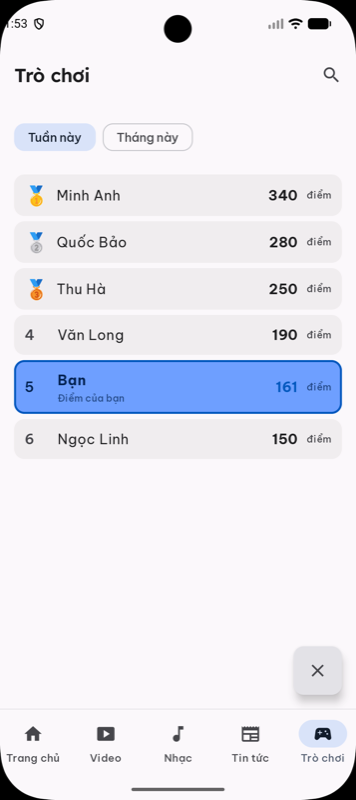
\includegraphics[width=2.75cm]{../figures/app/F-GAME-07-01.png}\hspace{0.25cm}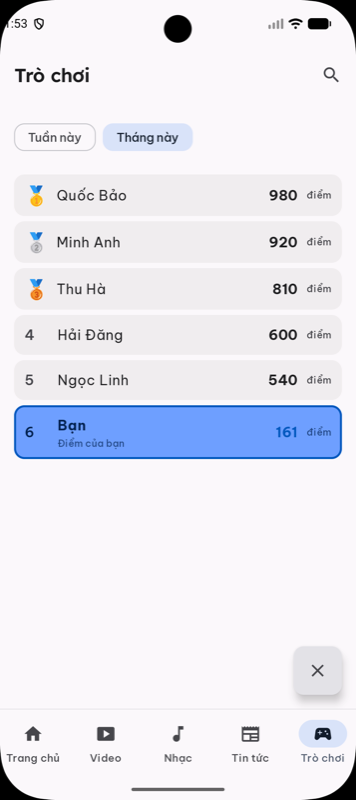
\includegraphics[width=2.75cm]{../figures/app/F-GAME-07-02.png}
\end{column}
\end{columns}
\end{frame}

\begin{frame}{Mock Up: Phân hệ Trò chơi}
\begin{columns}[T]
\begin{column}{0.46\textwidth}
{\small\bfseries\color{BKTemplate} F-GAME-08: Chơi game ở nửa dưới màn hình, video chạy phía trên}\\[2.5mm]
Tính năng thuộc nhóm Major Projects
\end{column}
\begin{column}{0.50\textwidth}
\centering
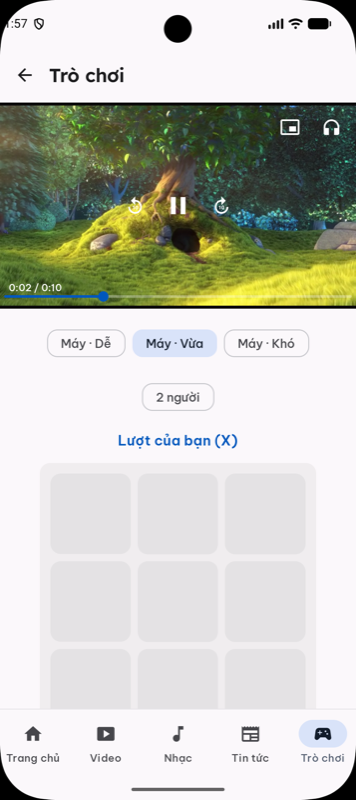
\includegraphics[height=6.1cm]{../figures/app/F-GAME-08-01.png}
\end{column}
\end{columns}
\end{frame}

\begin{frame}{Mock Up: Phân hệ Trò chơi}
\begin{columns}[T]
\begin{column}{0.46\textwidth}
{\small\bfseries\color{BKTemplate} F-GAME-09: Phần thưởng khi thắng minigame (điểm)}\\[2.5mm]
Tính năng thuộc nhóm Quick Wins
\end{column}
\begin{column}{0.50\textwidth}
\centering
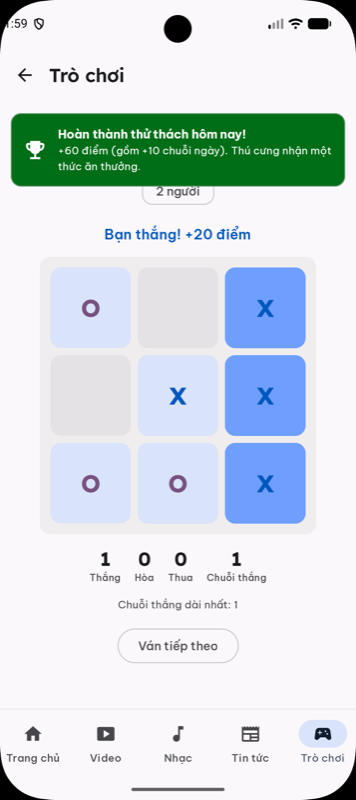
\includegraphics[height=6.1cm]{../figures/app/F-GAME-09-01.png}
\end{column}
\end{columns}
\end{frame}

\begin{frame}{Mock Up: Phân hệ Trò chơi}
\begin{columns}[T]
\begin{column}{0.46\textwidth}
{\small\bfseries\color{BKTemplate} F-GAME-10: 2048 (ghép số)}\\[2.5mm]
Tính năng thuộc nhóm Fill-ins
\end{column}
\begin{column}{0.50\textwidth}
\centering
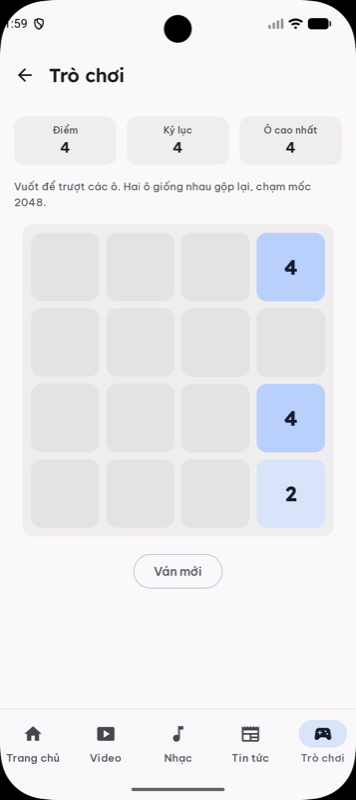
\includegraphics[height=6.1cm]{../figures/app/F-GAME-10-01.png}
\end{column}
\end{columns}
\end{frame}

\begin{frame}{Mock Up: Phân hệ Trò chơi}
\begin{columns}[T]
\begin{column}{0.46\textwidth}
{\small\bfseries\color{BKTemplate} F-GAME-11: Tic-Tac-Toe (caro 3$\times$3)}\\[2.5mm]
Tính năng thuộc nhóm Fill-ins
\end{column}
\begin{column}{0.50\textwidth}
\centering
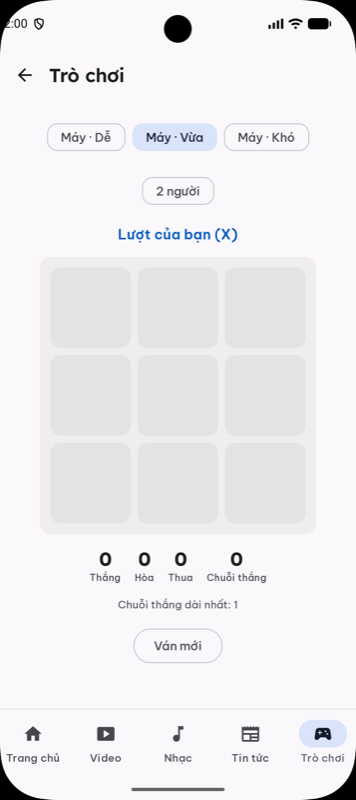
\includegraphics[width=2.75cm]{../figures/app/F-GAME-11-01.png}\hspace{0.25cm}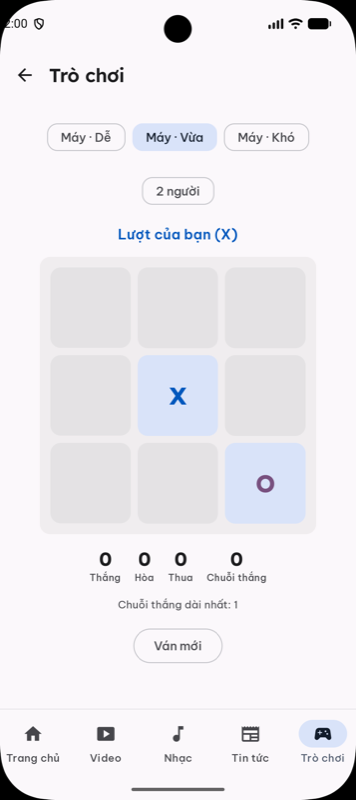
\includegraphics[width=2.75cm]{../figures/app/F-GAME-11-02.png}
\end{column}
\end{columns}
\end{frame}

\begin{frame}{Mock Up: Phân hệ Trò chơi}
\begin{columns}[T]
\begin{column}{0.46\textwidth}
{\small\bfseries\color{BKTemplate} F-GAME-12: Thử thách hằng ngày: xoay vòng 6 game, thưởng 50+5$\times$streak + thức ăn pet}\\[2.5mm]
Tính năng thuộc nhóm Quick Wins
\end{column}
\begin{column}{0.50\textwidth}
\centering
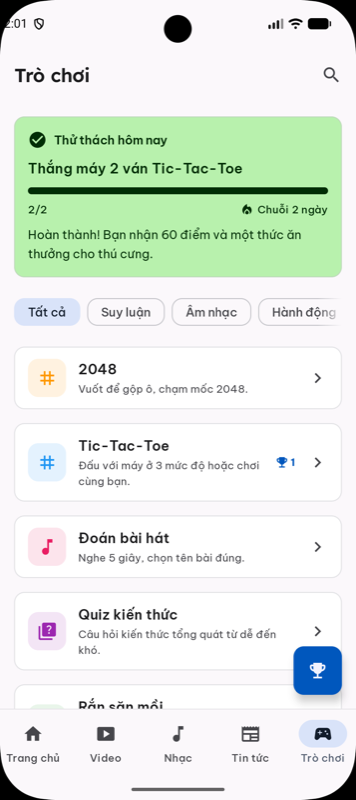
\includegraphics[height=6.1cm]{../figures/app/F-GAME-12-01.png}
\end{column}
\end{columns}
\end{frame}

\begin{frame}{Mock Up: Phân hệ Trò chơi}
\begin{columns}[T]
\begin{column}{0.46\textwidth}
{\small\bfseries\color{BKTemplate} F-GAME-13: Âm thanh và hiệu ứng game: âm phản hồi thao tác, tự giảm khi có nhạc/video}\\[2.5mm]
Tính năng thuộc nhóm Quick Wins
\end{column}
\begin{column}{0.50\textwidth}
\centering
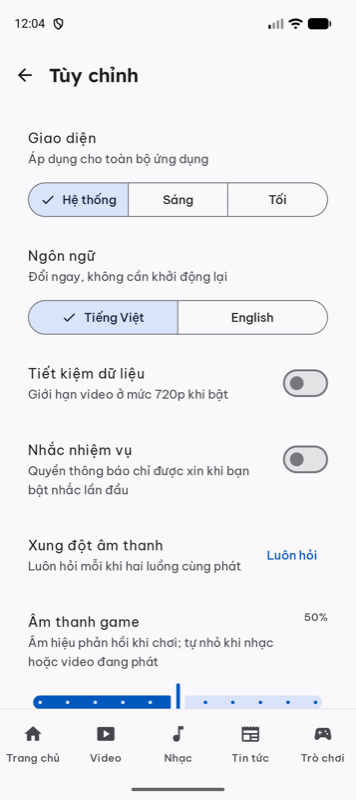
\includegraphics[height=6.1cm]{figures/app/F-GAME-13-01.png}
\end{column}
\end{columns}
\end{frame}

\begin{frame}{Mock Up: Dùng chung}
\begin{columns}[T]
\begin{column}{0.46\textwidth}
{\small\bfseries\color{BKTemplate} F-COM-01: Đăng ký/đăng nhập một tài khoản cho cả 4 phân hệ}\\[2.5mm]
Tính năng thuộc nhóm Major Projects
\end{column}
\begin{column}{0.50\textwidth}
\centering
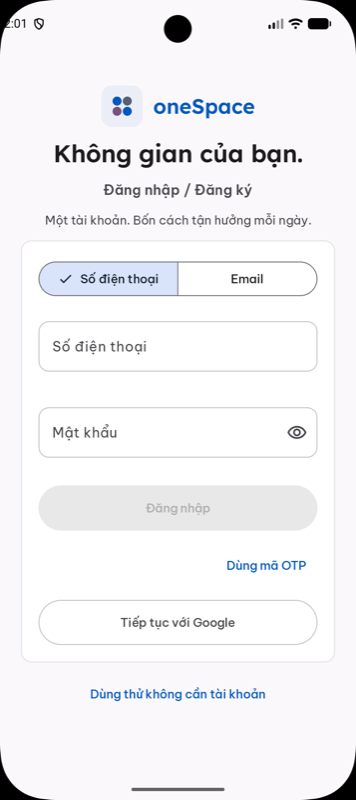
\includegraphics[width=2.32cm]{../figures/app/F-COM-01-01.png}\hspace{0.2cm}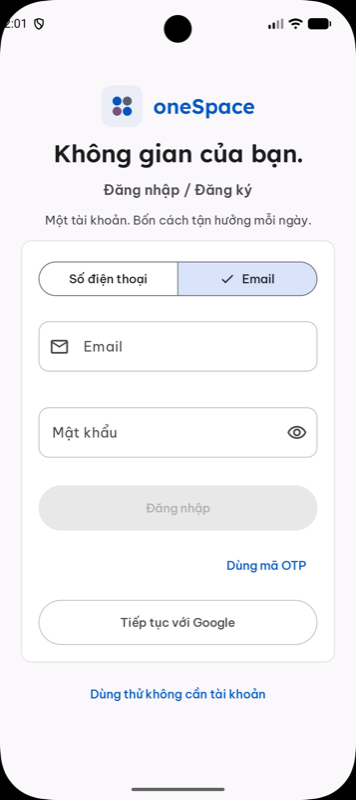
\includegraphics[width=2.32cm]{../figures/app/F-COM-01-02.png}\hspace{0.2cm}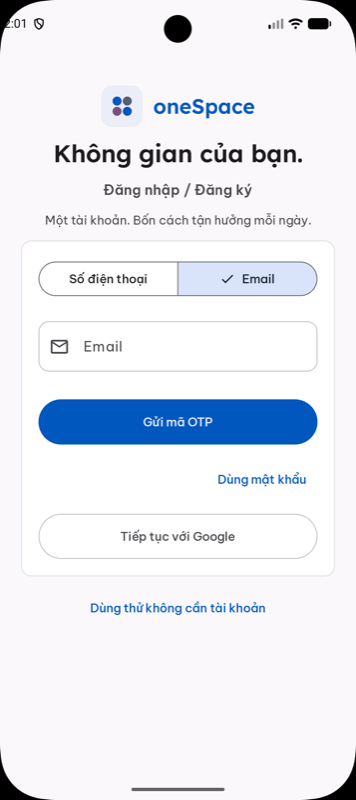
\includegraphics[width=2.32cm]{../figures/app/F-COM-01-03.png}
\end{column}
\end{columns}
\end{frame}

\begin{frame}{Mock Up: Dùng chung}
\begin{columns}[T]
\begin{column}{0.46\textwidth}
{\small\bfseries\color{BKTemplate} F-COM-02: Onboarding chọn sở thích lần đầu}\\[2.5mm]
Tính năng thuộc nhóm Quick Wins
\end{column}
\begin{column}{0.50\textwidth}
\centering
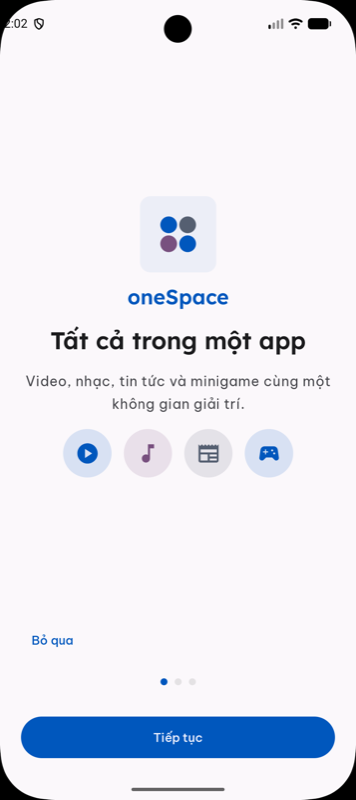
\includegraphics[width=2.32cm]{../figures/app/F-COM-02-01.png}\hspace{0.2cm}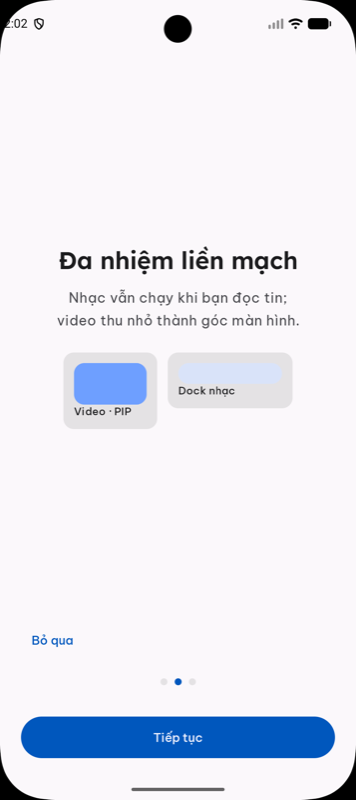
\includegraphics[width=2.32cm]{../figures/app/F-COM-02-02.png}\hspace{0.2cm}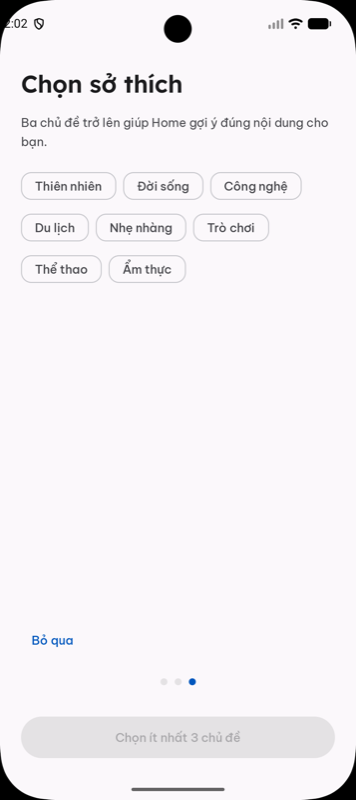
\includegraphics[width=2.32cm]{../figures/app/F-COM-02-03.png}
\end{column}
\end{columns}
\end{frame}

\begin{frame}{Mock Up: Dùng chung}
\begin{columns}[T]
\begin{column}{0.46\textwidth}
{\small\bfseries\color{BKTemplate} F-COM-03: Hồ sơ cá nhân: avatar, khung ảnh theo thành tích}\\[2.5mm]
Tính năng thuộc nhóm Fill-ins
\end{column}
\begin{column}{0.50\textwidth}
\centering
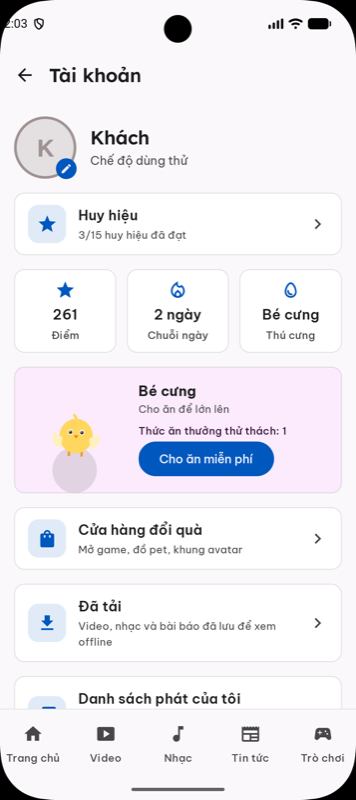
\includegraphics[width=2.75cm]{../figures/app/F-COM-03-01.png}\hspace{0.25cm}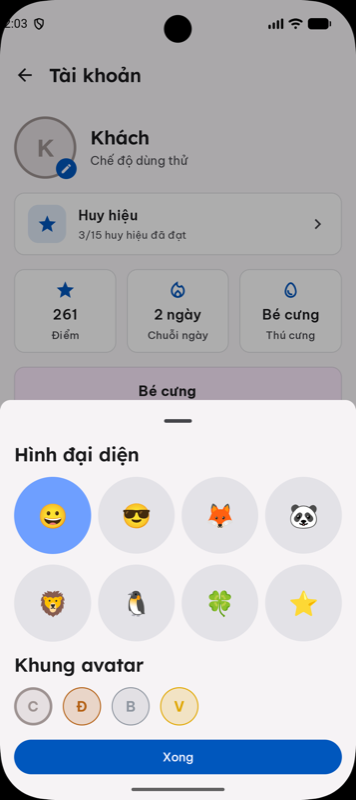
\includegraphics[width=2.75cm]{../figures/app/F-COM-03-02.png}
\end{column}
\end{columns}
\end{frame}

\begin{frame}{Mock Up: Dùng chung}
\begin{columns}[T]
\begin{column}{0.46\textwidth}
{\small\bfseries\color{BKTemplate} F-COM-04: Hệ điểm thưởng dùng chung (XP)}\\[2.5mm]
Tính năng thuộc nhóm Quick Wins
\end{column}
\begin{column}{0.50\textwidth}
\centering
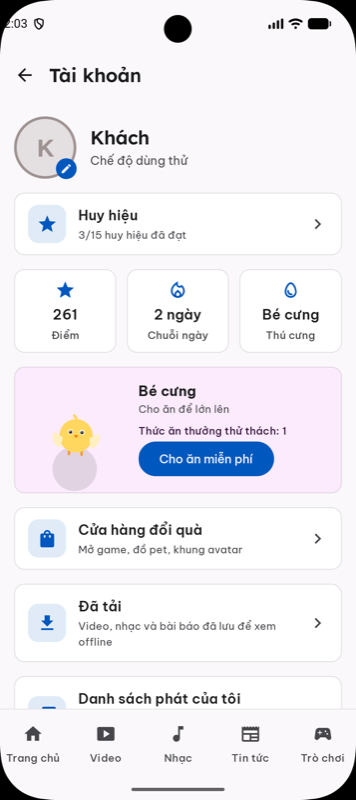
\includegraphics[width=2.75cm]{../figures/app/F-COM-04-01.png}\hspace{0.25cm}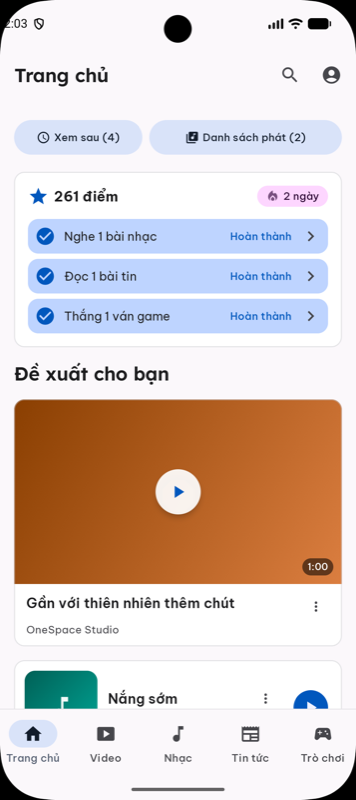
\includegraphics[width=2.75cm]{../figures/app/F-COM-04-02.png}
\end{column}
\end{columns}
\end{frame}

\begin{frame}{Mock Up: Dùng chung}
\begin{columns}[T]
\begin{column}{0.46\textwidth}
{\small\bfseries\color{BKTemplate} F-COM-05: Nhiệm vụ hằng ngày (3--5 nhiệm vụ)}\\[2.5mm]
Tính năng thuộc nhóm Quick Wins
\end{column}
\begin{column}{0.50\textwidth}
\centering
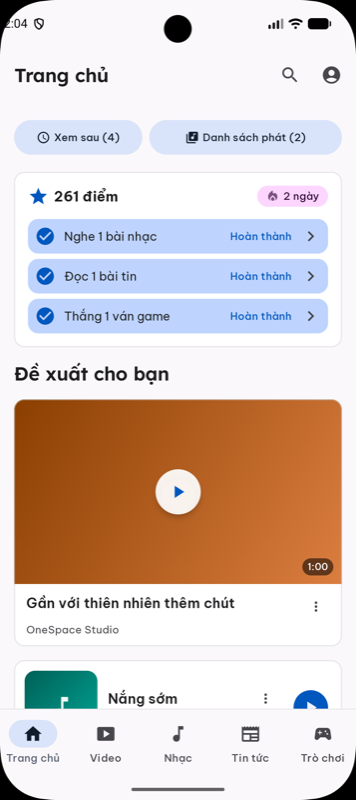
\includegraphics[height=6.1cm]{../figures/app/F-COM-05-01.png}
\end{column}
\end{columns}
\end{frame}

\begin{frame}{Mock Up: Dùng chung}
\begin{columns}[T]
\begin{column}{0.46\textwidth}
{\small\bfseries\color{BKTemplate} F-COM-06: Chuỗi ngày liên tiếp (streak)}\\[2.5mm]
Tính năng thuộc nhóm Quick Wins
\end{column}
\begin{column}{0.50\textwidth}
\centering
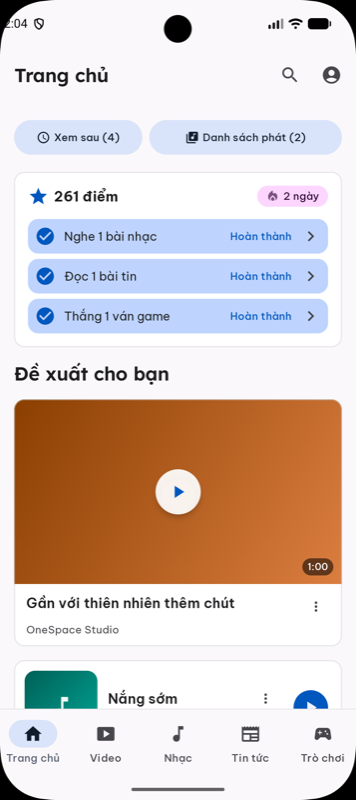
\includegraphics[height=6.1cm]{../figures/app/F-COM-06-01.png}
\end{column}
\end{columns}
\end{frame}

\begin{frame}{Mock Up: Dùng chung}
\begin{columns}[T]
\begin{column}{0.46\textwidth}
{\small\bfseries\color{BKTemplate} F-COM-07: Thú cưng ảo: nuôi bằng điểm, tiến hoá theo mốc}\\[2.5mm]
Tính năng thuộc nhóm Major Projects
\end{column}
\begin{column}{0.50\textwidth}
\centering
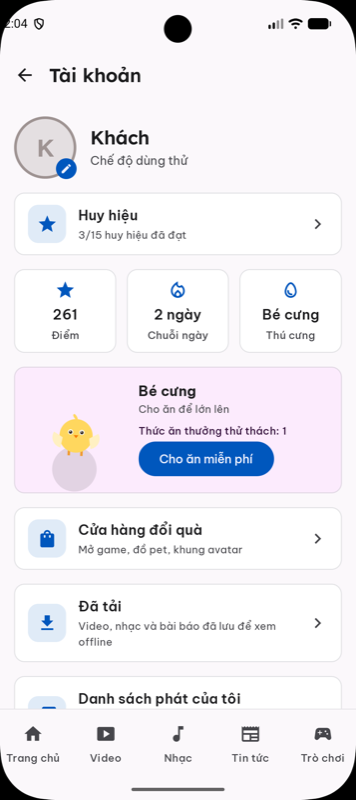
\includegraphics[width=2.75cm]{../figures/app/F-COM-07-01.png}\hspace{0.25cm}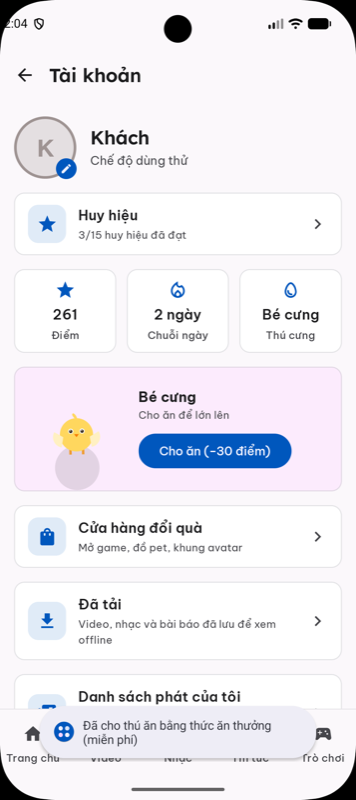
\includegraphics[width=2.75cm]{../figures/app/F-COM-07-02.png}
\end{column}
\end{columns}
\end{frame}

\begin{frame}{Mock Up: Dùng chung}
\begin{columns}[T]
\begin{column}{0.46\textwidth}
{\small\bfseries\color{BKTemplate} F-COM-08: Huy hiệu thành tựu}\\[2.5mm]
Tính năng thuộc nhóm Fill-ins
\end{column}
\begin{column}{0.50\textwidth}
\centering
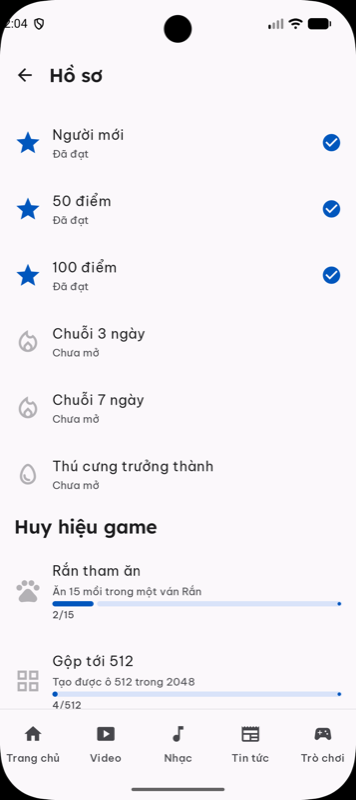
\includegraphics[height=6.1cm]{../figures/app/F-COM-08-01.png}
\end{column}
\end{columns}
\end{frame}

\begin{frame}{Mock Up: Dùng chung}
\begin{columns}[T]
\begin{column}{0.46\textwidth}
{\small\bfseries\color{BKTemplate} F-COM-09: Khung avatar độc quyền theo mốc thành tích}\\[2.5mm]
Tính năng thuộc nhóm Quick Wins
\end{column}
\begin{column}{0.50\textwidth}
\centering
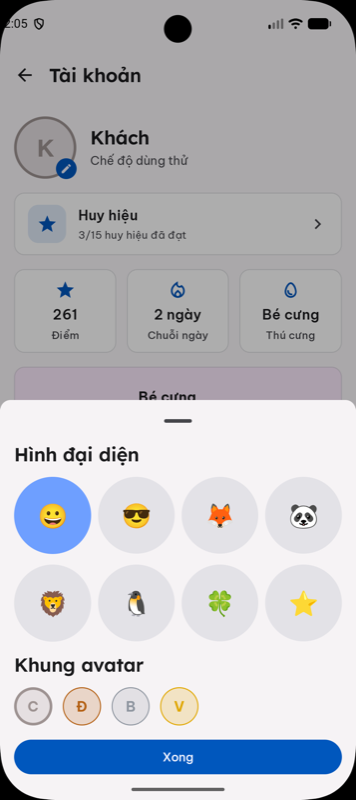
\includegraphics[height=6.1cm]{../figures/app/F-COM-09-01.png}
\end{column}
\end{columns}
\end{frame}

\begin{frame}{Mock Up: Dùng chung}
\begin{columns}[T]
\begin{column}{0.46\textwidth}
{\small\bfseries\color{BKTemplate} F-COM-10: Tổng kết tháng kiểu ``wrapped'', xuất thẻ chia sẻ}\\[2.5mm]
Tính năng thuộc nhóm Major Projects
\end{column}
\begin{column}{0.50\textwidth}
\centering
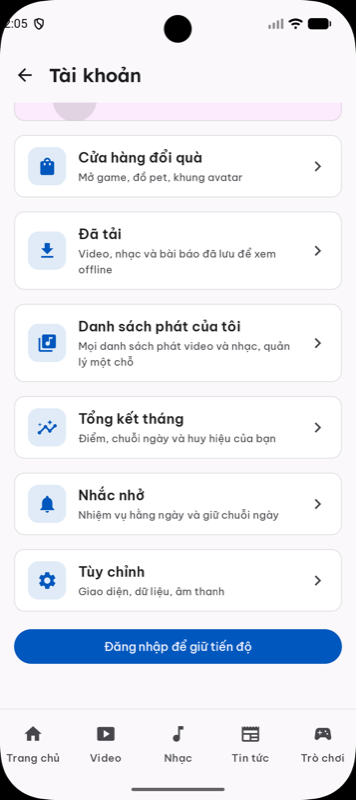
\includegraphics[width=2.32cm]{../figures/app/F-COM-10-01.png}\hspace{0.2cm}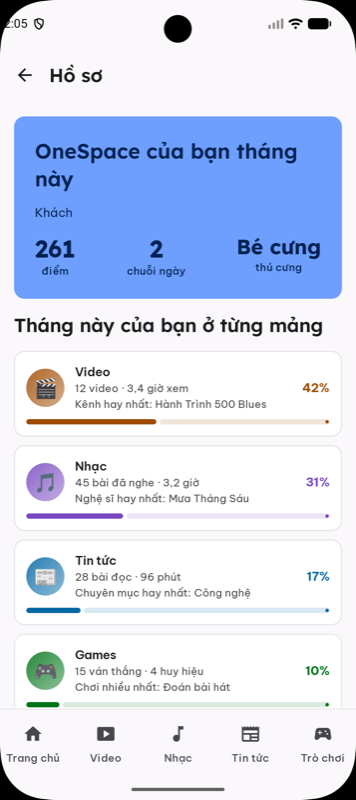
\includegraphics[width=2.32cm]{../figures/app/F-COM-10-02.png}\hspace{0.2cm}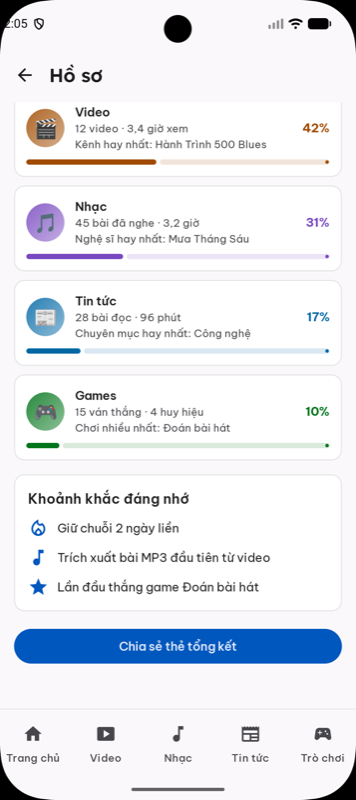
\includegraphics[width=2.32cm]{../figures/app/F-COM-10-03.png}
\end{column}
\end{columns}
\end{frame}

\begin{frame}{Mock Up: Dùng chung}
\begin{columns}[T]
\begin{column}{0.46\textwidth}
{\small\bfseries\color{BKTemplate} F-COM-11: Tìm kiếm xuyên nội dung (một ô tìm cho 4 phân hệ)}\\[2.5mm]
Tính năng thuộc nhóm Major Projects
\end{column}
\begin{column}{0.50\textwidth}
\centering
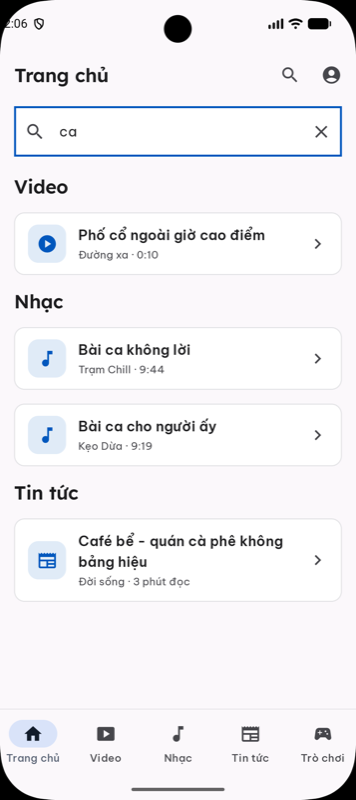
\includegraphics[height=6.1cm]{../figures/app/F-COM-11-01.png}
\end{column}
\end{columns}
\end{frame}

\begin{frame}{Mock Up: Dùng chung}
\begin{columns}[T]
\begin{column}{0.46\textwidth}
{\small\bfseries\color{BKTemplate} F-COM-12: Nhắc nhiệm vụ/streak hằng ngày}\\[2.5mm]
Tính năng thuộc nhóm Quick Wins
\end{column}
\begin{column}{0.50\textwidth}
\centering
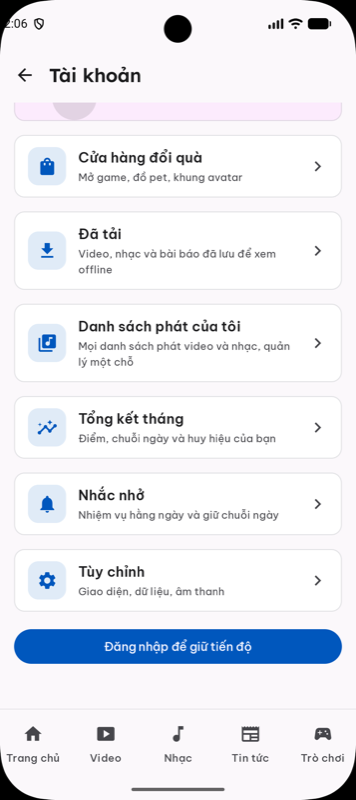
\includegraphics[width=2.75cm]{../figures/app/F-COM-12-01.png}\hspace{0.25cm}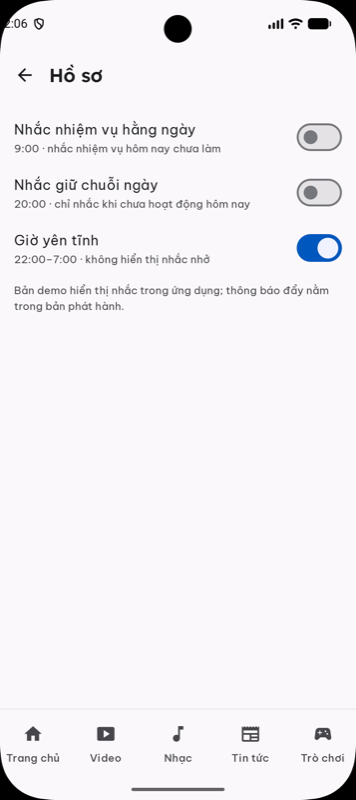
\includegraphics[width=2.75cm]{../figures/app/F-COM-12-02.png}
\end{column}
\end{columns}
\end{frame}

\begin{frame}{Mock Up: Dùng chung}
\begin{columns}[T]
\begin{column}{0.46\textwidth}
{\small\bfseries\color{BKTemplate} F-COM-13: Cài đặt: sáng/tối, ngôn ngữ, tiết kiệm dữ liệu}\\[2.5mm]
Tính năng thuộc nhóm Quick Wins
\end{column}
\begin{column}{0.50\textwidth}
\centering
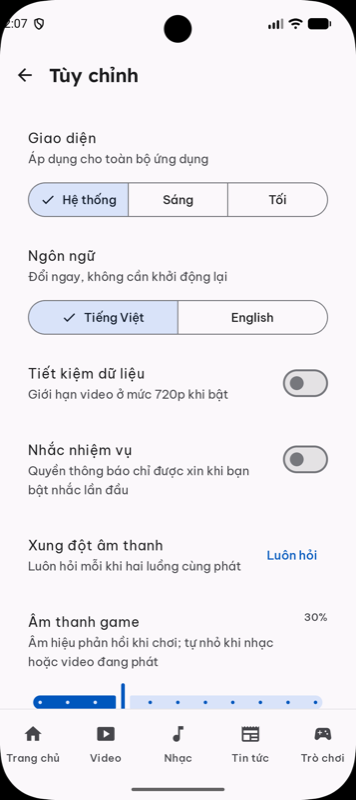
\includegraphics[width=2.75cm]{../figures/app/F-COM-13-01.png}\hspace{0.25cm}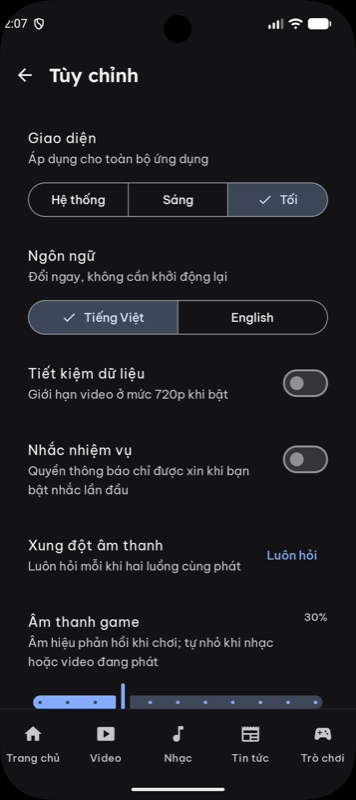
\includegraphics[width=2.75cm]{../figures/app/F-COM-13-02.png}
\end{column}
\end{columns}
\end{frame}

\begin{frame}{Mock Up: Dùng chung}
\begin{columns}[T]
\begin{column}{0.46\textwidth}
{\small\bfseries\color{BKTemplate} F-COM-14: Cửa sổ xác nhận khi hai luồng âm thanh xung đột}\\[2.5mm]
Tính năng thuộc nhóm Quick Wins
\end{column}
\begin{column}{0.50\textwidth}
\centering
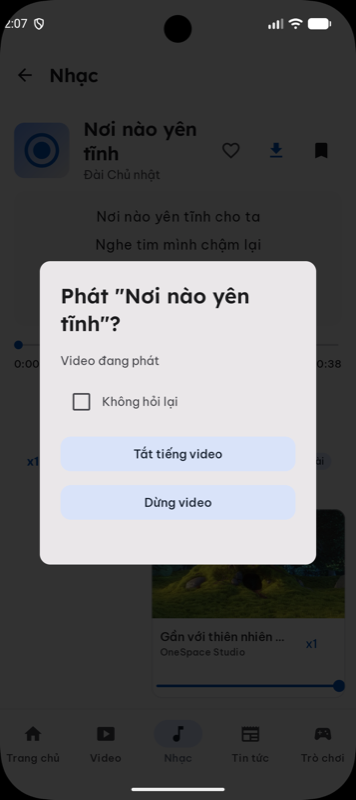
\includegraphics[width=2.75cm]{../figures/app/F-COM-14-01.png}\hspace{0.25cm}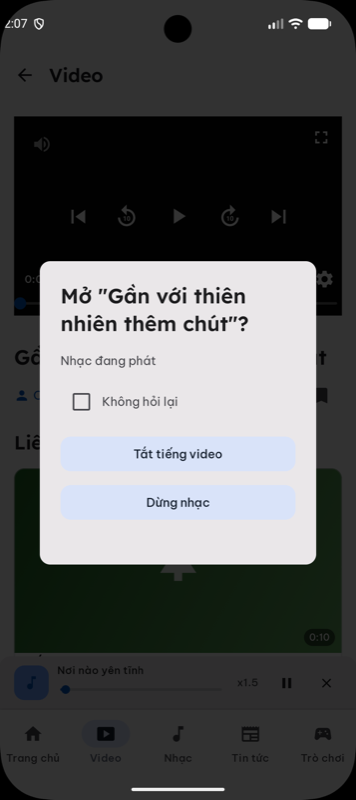
\includegraphics[width=2.75cm]{../figures/app/F-COM-14-02.png}
\end{column}
\end{columns}
\end{frame}

\begin{frame}{Mock Up: Dùng chung}
\begin{columns}[T]
\begin{column}{0.46\textwidth}
{\small\bfseries\color{BKTemplate} F-COM-15: Cửa hàng đổi quà bằng điểm (mở game, đồ pet, khung avatar)}\\[2.5mm]
Tính năng thuộc nhóm Quick Wins
\end{column}
\begin{column}{0.50\textwidth}
\centering
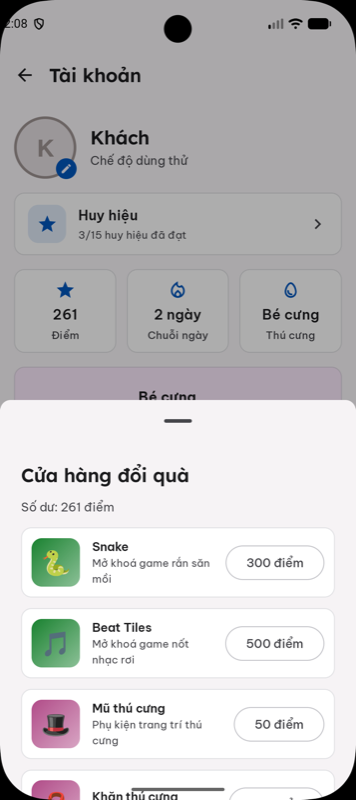
\includegraphics[height=6.1cm]{../figures/app/F-COM-15-01.png}
\end{column}
\end{columns}
\end{frame}

\begin{frame}{Mock Up: Dùng chung}
\begin{columns}[T]
\begin{column}{0.46\textwidth}
{\small\bfseries\color{BKTemplate} F-COM-16: Chế độ ngoại tuyến cơ bản: tin đã lưu, trạng thái mất mạng}\\[2.5mm]
Tính năng thuộc nhóm Major (hoãn tới gần cuối)
\end{column}
\begin{column}{0.50\textwidth}
\centering
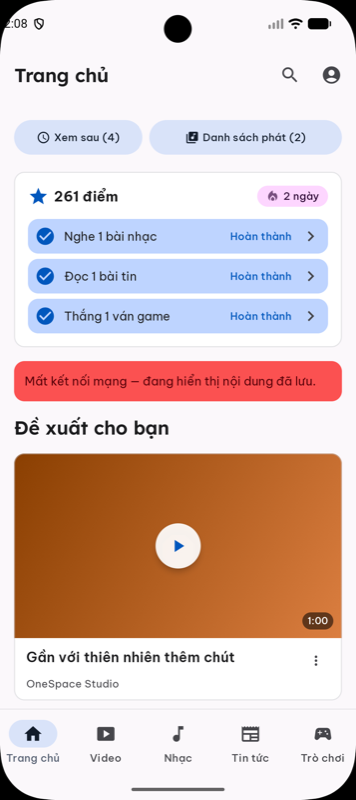
\includegraphics[width=2.75cm]{../figures/app/F-COM-16-01.png}\hspace{0.25cm}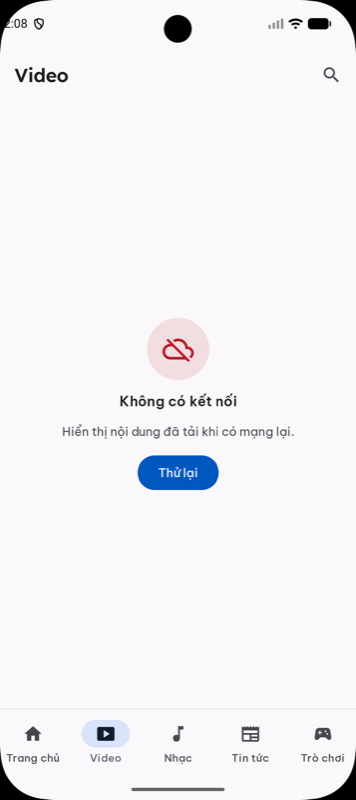
\includegraphics[width=2.75cm]{../figures/app/F-COM-16-02.png}
\end{column}
\end{columns}
\end{frame}

\begin{frame}{Mock Up: Dùng chung}
\begin{columns}[T]
\begin{column}{0.46\textwidth}
{\small\bfseries\color{BKTemplate} F-COM-18: Chế độ khách dùng thử (không cần tài khoản)}\\[2.5mm]
Tính năng thuộc nhóm Quick Wins
\end{column}
\begin{column}{0.50\textwidth}
\centering
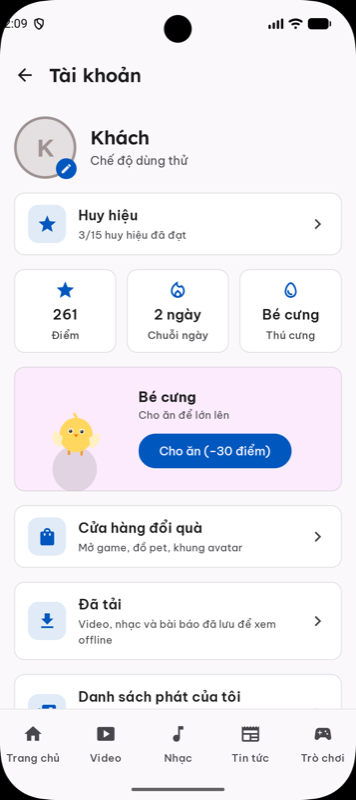
\includegraphics[width=2.75cm]{../figures/app/F-COM-18-01.png}\hspace{0.25cm}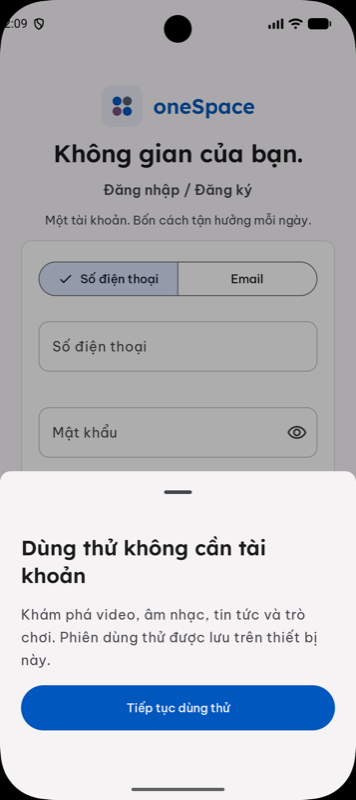
\includegraphics[width=2.75cm]{../figures/app/F-COM-18-02.png}
\end{column}
\end{columns}
\end{frame}

\begin{frame}{Mock Up: Dùng chung}
\begin{columns}[T]
\begin{column}{0.46\textwidth}
{\small\bfseries\color{BKTemplate} F-COM-19: Karaoke/Record: ghi màn hình video (MediaProjection), countdown 3-2-1}\\[2.5mm]
Tính năng thuộc nhóm Major Projects
\end{column}
\begin{column}{0.50\textwidth}
\centering
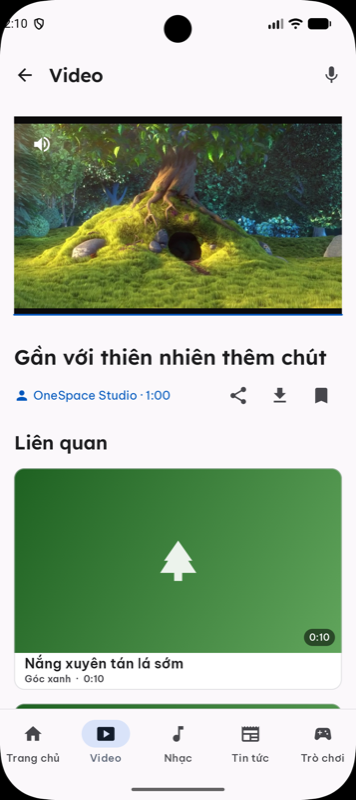
\includegraphics[width=2.32cm]{../figures/app/F-COM-19-01.png}\hspace{0.2cm}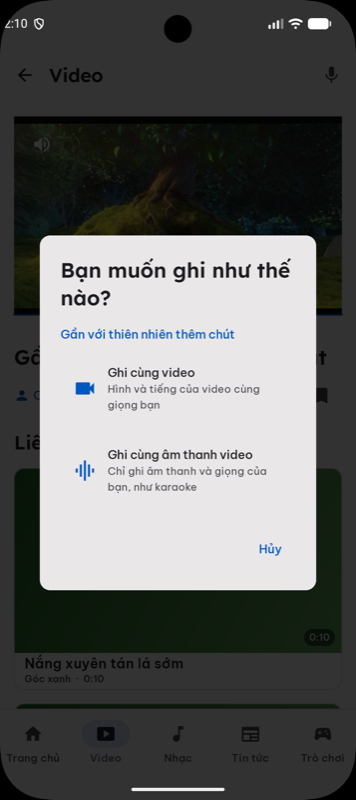
\includegraphics[width=2.32cm]{../figures/app/F-COM-19-02.png}\hspace{0.2cm}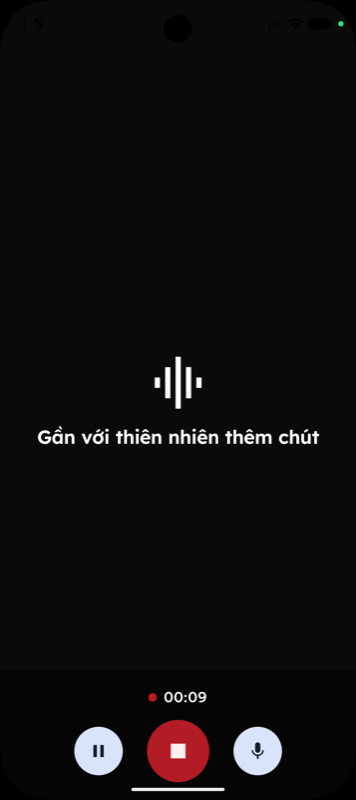
\includegraphics[width=2.32cm]{../figures/app/F-COM-19-03.png}
\end{column}
\end{columns}
\end{frame}

\begin{frame}{Mock Up: Dùng chung}
\begin{columns}[T]
\begin{column}{0.46\textwidth}
{\small\bfseries\color{BKTemplate} F-COM-20: Vuốt ngang đổi phân hệ (trừ Games) + hoàn tác đóng nhạc}\\[2.5mm]
Tính năng thuộc nhóm Quick Wins
\end{column}
\begin{column}{0.50\textwidth}
\centering
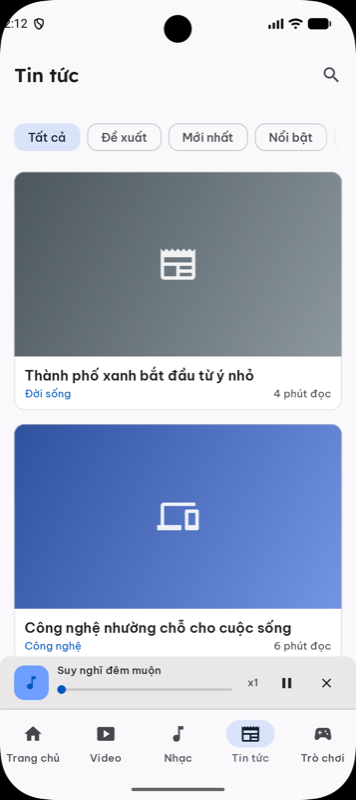
\includegraphics[height=6.1cm]{../figures/app/F-COM-20-01.png}
\end{column}
\end{columns}
\end{frame}

\begin{frame}{Mock Up: Dùng chung}
\begin{columns}[T]
\begin{column}{0.46\textwidth}
{\small\bfseries\color{BKTemplate} F-COM-21: Ghi âm, hát karaoke cùng bài hát đang phát (bên Nhạc)}\\[2.5mm]
Tính năng thuộc nhóm Major Projects
\end{column}
\begin{column}{0.50\textwidth}
\centering
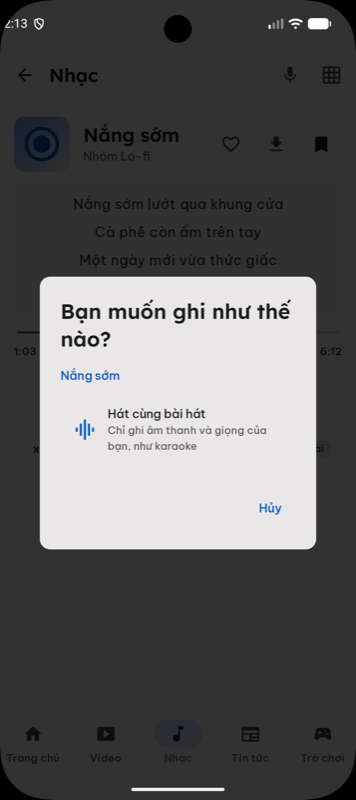
\includegraphics[height=6.1cm]{../figures/app/F-COM-21-01.png}
\end{column}
\end{columns}
\end{frame}

% ===== END MOCKUP =====








\subsection{Design System: Token màu theo vai trò}
% ------------------------------------------------------------
\begin{frame}{Design System --- Token màu theo vai trò}
\begin{columns}[T]
\begin{column}{0.48\textwidth}
{\small\textbf{Màu chính \& nhấn (Light)}}\vspace{1mm}
{\tiny
\begin{itemize}\setlength{\itemsep}{3pt}
\item \sw{0057BD}{F0F2FF} \texttt{primary} 0057BD / dark 85ADFF \newline Nút chính; tab đang chọn; chữ ``Đang phát''; logo
\item \sw{6E9FFF}{001B3F} \texttt{primaryContainer} 6E9FFF \newline Nền icon ContentCard; ô quiz đúng; huy hiệu; nhiệm vụ xong
\item \sw{555F71}{FFFFFF} \texttt{secondary} 555F71 / BDC7DC \newline Icon onboarding; màu phụ logo
\item \sw{78507F}{FFFFFF} \texttt{tertiary} 78507F / E7B6EC \newline Icon streak; nhãn ``Đã xem đến''
\item \sw{FDD6FF}{5E3966} \texttt{tertiaryContainer} FDD6FF / 5E3966 \newline Chip chuỗi ngày; card thú cưng
\item \sw{B31B25}{FFFFFF} \texttt{error} B31B25 / FF716C \newline Lỗi phát; quiz sai; icon yêu thích (tim đỏ)
\end{itemize}}
\end{column}
\begin{column}{0.48\textwidth}
{\small\textbf{Nền, bề mặt \& viền (Light)}}\vspace{1mm}
{\tiny
\begin{itemize}\setlength{\itemsep}{3pt}
\item \sw{FBF8FB}{131315} \texttt{background}/\texttt{surface} FBF8FB / 131315 \newline Nền mọi màn hình; nền card đang kéo (queue)
\item \sw{E3E2E7}{333539} \texttt{surfaceVariant} E3E2E7 / 333539 \newline Ô làn Beat Tiles; nền avatar chưa chọn
\item \sw{EAE7E9}{2A2A2C} \texttt{surfaceContainerHigh} EAE7E9 / 2A2A2C \newline Nền thẻ nổi: banner nhiệm vụ, khung đăng nhập
\item \sw{76777C}{909095} \texttt{outline} 76777C / 909095 \newline Icon radio chưa chọn; vạch phân tách TrackCard
\end{itemize}}
\vspace{1.5mm}
{\tiny
\begin{itemize}\setlength{\itemsep}{3pt}
\item Design system của ứng dụng được xây trên \textbf{Material 3}
\item Mã nguồn không hardcode màu, mọi màn hình đều tham chiếu \textbf{Material Theme}
\end{itemize}}
\end{column}
\end{columns}
\end{frame}

% ------------------------------------------------------------
\subsection{Typography}
% ------------------------------------------------------------
\begin{frame}{Typography --- Nguyên thang chữ Material 3}
\begin{columns}[T]
\begin{column}{0.58\textwidth}
{\tiny\color{TextGray} display $\cdot$ 57sp $\cdot$ splash logo}\\[1pt]
{\fontsize{22}{25}\selectfont\bfseries OneSpace}\\[7pt]
{\tiny\color{TextGray} headline $\cdot$ 24--28sp $\cdot$ tiêu đề màn}\\[1pt]
{\fontsize{14.5}{17}\selectfont\bfseries Thư viện}\\[6pt]
{\tiny\color{TextGray} title $\cdot$ 14--16sp $\cdot$ tiêu đề card, tab}\\[1pt]
{\fontsize{11}{13}\selectfont Nắng sớm}\\[6pt]
{\tiny\color{TextGray} body $\cdot$ 14sp $\cdot$ nội dung, mô tả}\\[1pt]
{\fontsize{9}{11}\selectfont Nhóm Lo-fi $\cdot$ 9:19}\\[6pt]
{\tiny\color{TextGray} label $\cdot$ 11--14sp $\cdot$ chip, nhãn phụ, badge}\\[2pt]
\colorbox[HTML]{E3E2E7}{\textcolor[HTML]{131315}{\fontsize{7.5}{9.5}\selectfont~Tất cả~}}\;\;
{\fontsize{7.5}{9.5}\selectfont\textcolor[HTML]{0057BD}{Đang phát}}\\[9pt]
{\tiny
\begin{itemize}\setlength{\itemsep}{2pt}
\item Nguyên thang M3 (display, headline, title, body, label), không font riêng
\item Đơn vị \texttt{sp} $\rightarrow$ phóng theo cỡ chữ hệ thống
\item Trình đọc bài: riêng 2 nút A$-$/A$+$ (0,8x--1,6x, bước 15\%)
\end{itemize}}
\end{column}
\begin{column}{0.38\textwidth}
\centering
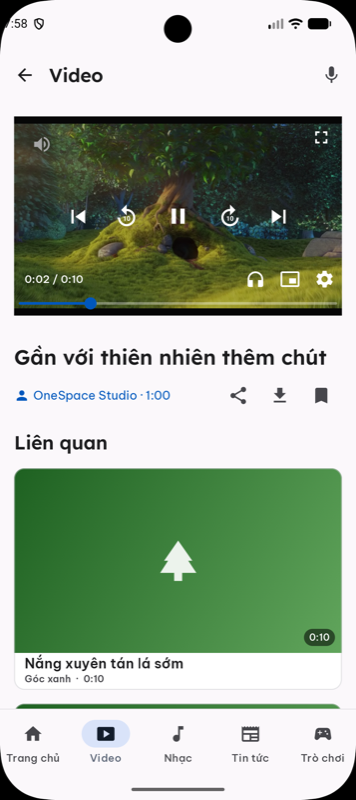
\includegraphics[height=170pt]{../figures/app/F-VID-01-02.png}\\[3pt]
{\tiny\color{TextGray} Màn hình thật}
\end{column}
\end{columns}
\end{frame}

% ------------------------------------------------------------
\subsection{Component}
% ------------------------------------------------------------
\begin{frame}{Component --- Ba nhóm chức năng}
\noindent\begin{minipage}{\textwidth}
{\tiny\color{TextGray} Input control $\cdot$ Navigation $\cdot$ Information --- ảnh chụp từ ứng dụng OneSpace}
\end{minipage}\vspace{2mm}

\begin{columns}[T]
\begin{column}{0.31\textwidth}
\centering
{\small\textbf{1. Input control}}\\[1.5mm]
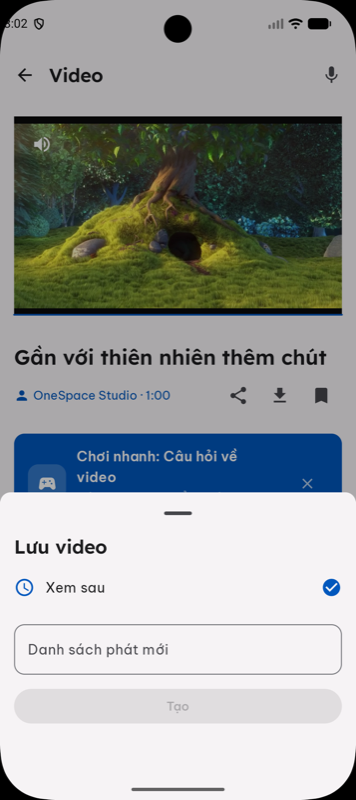
\includegraphics[height=88pt]{../figures/app/F-VID-04-01.png}\\[1.5mm]
{\tiny\color{TextGray} Bảng cài đặt trình phát}\\[1mm]
{\tiny
\begin{itemize}\setlength{\itemsep}{2pt}
\item Ô OTP / mật khẩu
\item Thanh trượt: tốc độ 0,5--2x, âm lượng
\item Chip chất lượng: Auto / 1080p / 720p / 360p
\item Ô tick ``Không hỏi lại''
\end{itemize}}
\end{column}
\begin{column}{0.31\textwidth}
\centering
{\small\textbf{2. Navigation}}\\[1.5mm]
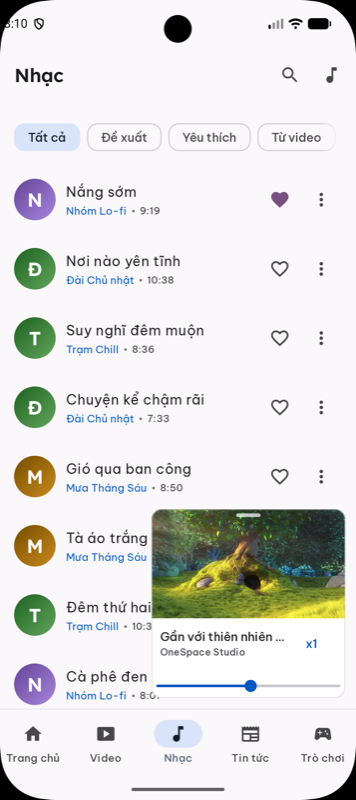
\includegraphics[height=88pt]{../figures/app/F-VID-08-01.png}\\[1.5mm]
{\tiny\color{TextGray} Màn Home --- thanh tab dưới đáy}\\[1mm]
{\tiny
\begin{itemize}\setlength{\itemsep}{2pt}
\item Bottom Nav 5 tab
\item Vuốt ngang đổi phân hệ
\item Nút Quay lại
\item Kéo dock nhạc lên mở hàng đợi
\end{itemize}}
\end{column}
\begin{column}{0.31\textwidth}
\centering
{\small\textbf{3. Information / Container}}\\[1.5mm]
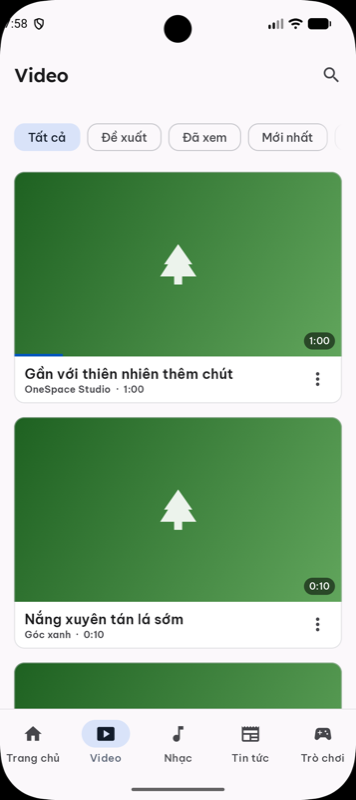
\includegraphics[height=88pt]{../figures/app/F-VID-01-01.png}\\[1.5mm]
{\tiny\color{TextGray} Feed Video --- thẻ nội dung dùng chung}\\[1mm]
{\tiny
\begin{itemize}\setlength{\itemsep}{2pt}
\item ContentCard (thẻ 4 phân hệ)
\item Skeleton feed khi tải
\item Snackbar thông báo
\item Modal Bottom Sheet (hàng đợi, chọn khung)
\end{itemize}}
\end{column}
\end{columns}
\vspace{1.5mm}
{\tiny\textbf{Thư viện dùng chung} (module \texttt{design system}): \texttt{FeaturePage} $\cdot$ \texttt{SectionTitle} $\cdot$ \texttt{ContentCard} $\cdot$ \texttt{CatalogContent} $\cdot$ \texttt{SkeletonFeed} $\cdot$ \texttt{EmptyState}}
\end{frame}

% ------------------------------------------------------------
\subsection{Trạng thái phụ}
% ------------------------------------------------------------
\begin{frame}{Trạng thái phụ: đang tải, trống, lỗi, ngoại tuyến}
\begin{columns}[T]
\begin{column}{0.55\textwidth}
{\small\textbf{Mọi feed dùng chung một bộ chuyển trạng thái}}\\[1.5mm]
{\footnotesize
\begin{itemize}\setlength{\itemsep}{4pt}
\item \textbf{Đang tải:} skeleton 4 hàng + hiệu ứng shimmer, không spinner toàn màn
\item \textbf{Trống:} icon + thông điệp + nút hành động (EmptyState)
\item \textbf{Lỗi:} ``Không tải được'' + nút ``Thử lại'' ở giữa màn hình
\item \textbf{Mất mạng:} banner ``Mất kết nối'' trên Home, nội dung đã lưu vẫn đọc được; có mạng tự phục hồi
\item Ván game cục bộ vẫn chơi được khi offline
\end{itemize}}
\end{column}
\begin{column}{0.41\textwidth}
\centering
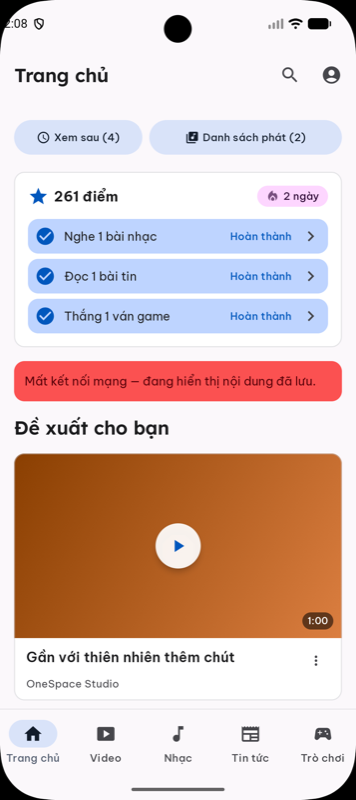
\includegraphics[height=4.1cm]{../figures/app/F-COM-16-01.png}\hspace{1mm}
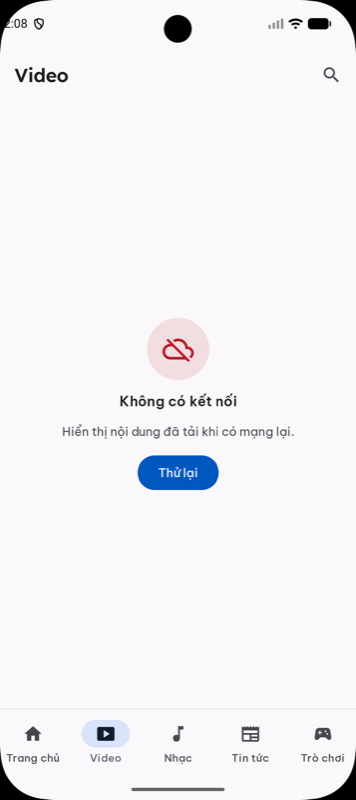
\includegraphics[height=4.1cm]{../figures/app/F-COM-16-02.png}\hspace{1mm}
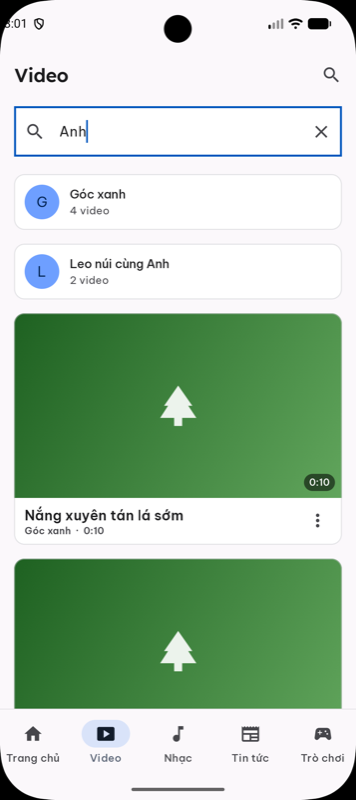
\includegraphics[height=4.1cm]{../figures/app/F-VID-03-02.png}\\[1mm]
{\tiny\color{TextGray} Trạng thái mất mạng (F-COM-16) $\cdot$ tìm kiếm không có kết quả (F-VID-03)}
\end{column}
\end{columns}
\end{frame}

% ------------------------------------------------------------
\subsection{Accessibility}
% ------------------------------------------------------------
\begin{frame}{Accessibility}
\begin{columns}[T]
\begin{column}{0.48\textwidth}
{\small\textbf{Vùng chạm $\geq$ 48$\times$48 dp}}\vspace{1mm}
{\tiny
\begin{itemize}\setlength{\itemsep}{2pt}
\item Mọi nút dùng component M3 $\rightarrow$ tự kế thừa
\item Thẻ nội dung cao $>$ 48dp
\item Ô bàn chơi 2048: 4$\times$4 ô, mỗi ô $>$ 48dp
\end{itemize}}\vspace{2mm}
{\small\textbf{Tương phản màu (WCAG 2.x)}}\vspace{1mm}
{\tiny
\begin{tabular}{@{}lll@{}}
\toprule
\textbf{Cặp} & \textbf{Light} & \textbf{Dark} \\
\midrule
onBackground/bg & 16,3:1 & 14,4:1 \\
onPrimary/primary & 6,4:1 & 7,6:1 \\
onSurfaceVar/surface & 8,9:1 & 10,9:1 \\
outline/bg & 4,3:1 & 5,8:1 \\
\bottomrule
\end{tabular}}
\end{column}
\begin{column}{0.48\textwidth}
{\small\textbf{Ví dụ cặp màu đạt AA}}\vspace{1mm}

\colorbox[HTML]{FBF8FB}{\textcolor[HTML]{131315}{\rule{0pt}{0.28cm}~Nền sáng, chữ tối --- 16,3:1 \textcolor{GreenOK}{\checkmark}~}}\\[3pt]
\colorbox[HTML]{131315}{\textcolor[HTML]{FBF8FB}{\rule{0pt}{0.28cm}~Nền tối, chữ sáng --- 14,4:1 \textcolor{GreenOK}{\checkmark}~}}\\[3pt]
\colorbox[HTML]{0057BD}{\textcolor[HTML]{F0F2FF}{\rule{0pt}{0.28cm}~Nút chính, onPrimary --- 6,4:1 \textcolor{GreenOK}{\checkmark}~}}\\[3pt]
\colorbox[HTML]{B31B25}{\textcolor[HTML]{FFFFFF}{\rule{0pt}{0.28cm}~Nút lỗi, onError --- 6,5:1 \textcolor{GreenOK}{\checkmark}~}}
\vspace{2.5mm}

{\small\textbf{Chữ và trình đọc màn hình}}\vspace{1mm}
{\tiny
\begin{itemize}\setlength{\itemsep}{2pt}
\item Toàn bộ chữ dùng đơn vị sp~--~theo cỡ chữ hệ thống; trình đọc bài có A$-$/A$+$ 0,8x--1,6x
\item TalkBack: nhãn đã thêm ở Account, Nhạc, Tin; thẻ game và một số nút icon chưa đủ~--~tự đánh giá chưa đạt, xếp v2
\end{itemize}}
\end{column}
\end{columns}
\end{frame}

% ------------------------------------------------------------
\subsection{Micro-interactions}
% ------------------------------------------------------------
\begin{frame}{Micro-interactions --- Mô hình Saffer 4 thành phần}
\begin{center}
\begin{tikzpicture}[
    font=\scriptsize,
    comp/.style={draw=BKTemplate, thick, rounded corners=3pt, fill=BKTemplate!8, minimum height=10mm, minimum width=2.4cm, align=center},
    arrow/.style={-{Latex[length=2mm]}, BKTemplate!60, thick}]
  \node[comp] (trg) at (0,0) {\textbf{Trigger}\\Người dùng làm gì};
  \node[comp, right=1.5cm of trg] (rul) {\textbf{Rules}\\Điều kiện áp};
  \node[comp, right=1.5cm of rul] (fdb) {\textbf{Feedback}\\Người dùng thấy gì};
  \node[comp, below=1.2cm of fdb] (lp) {\textbf{Loops \& Modes}\\Hành vi lặp / giới hạn};
  \draw[arrow] (trg) -- (rul);
  \draw[arrow] (rul) -- (fdb);
  \draw[arrow] (fdb) -- (lp);
  \draw[arrow] (lp.west) -- ++(-8.1,0) -- ++(0,3.2) -- (0,0.98) -- (trg.north);
\end{tikzpicture}
\end{center}
\end{frame}

\begin{frame}{Micro-interactions --- Các tương tác đã cài}
\begin{columns}[T]
\begin{column}{0.48\textwidth}
{\scriptsize\textbf{Tải và điều hướng}}\vspace{1mm}
{\tiny
\begin{itemize}\setlength{\itemsep}{2.5pt}
\item \textbf{Skeleton feed:} vào feed khi dữ liệu đang tải, bốn hàng khung xám kèm hiệu ứng shimmer; khung biến mất ngay khi có dữ liệu
\item \textbf{Ripple Material:} mọi nút, thẻ, tab phản hồi bằng vòng sóng lan từ điểm chạm; mặc định toàn hệ thống
\item \textbf{Vuốt ngang:} vuốt trái/phải trên màn feed chuyển sang phân hệ kế bên, giữ nguyên trạng thái từng phân hệ; tắt trong game vì cử chỉ dành cho điều khiển ván chơi
\item \textbf{Dock mini player:} bài đang phát hiện một hàng dock ở đáy mọi màn (kể cả trình đọc bài); chạm mở trình phát đầy đủ
\item \textbf{Cửa sổ nổi:} rời tab khi video đang phát, video thu nhỏ thành cửa sổ ở góc kèm nhãn ``Đang phát'' và ba nút Mở rộng, Tạm dừng, Đóng
\end{itemize}}
\end{column}
\begin{column}{0.48\textwidth}
{\scriptsize\textbf{Tương tác nội dung}}\vspace{1mm}
{\tiny
\begin{itemize}\setlength{\itemsep}{2.5pt}
\item \textbf{Popup C1:} mở nhạc khi video đang phát: hộp thoại hai lựa chọn kèm ô tick ``Không hỏi lại''; không có nút bỏ qua, phải chọn một
\item \textbf{Trạng thái rỗng:} danh mục không có nội dung hiển thị biểu tượng, thông điệp và nút hành động; không để màn hình trống không lối đi
\item \textbf{Mất mạng:} feed không tải được hiện ``Không có kết nối'' kèm nút ``Thử lại''; khi có mạng tự phục hồi
\item \textbf{Bàn chơi 2048:} ô cùng giá trị gộp nhau theo hướng vuốt, bàn chơi và điểm cập nhật tức thì sau mỗi nước
\item \textbf{Beat Tiles:} nốt rơi bốn làn, chạm đúng ô khi nốt vào vùng sáng; điểm và combo tăng tức thì, nhạc vẫn phát
\end{itemize}}
\end{column}
\end{columns}
\end{frame}

% ============================================================
% SECTION 4 - KIẾN TRÚC KỸ THUẬT
% Nền tảng · Kiến trúc ba lớp · Mô-đun · Điều hướng
% Dữ liệu · Upload & phát · Lưu trữ · Phối hợp media · TTS
% ============================================================
\section{Kiến trúc kỹ thuật}

% ------------------------------------------------------------
\subsection{Nền tảng và lựa chọn kỹ thuật}
% ------------------------------------------------------------
\begin{frame}{Nền tảng và lựa chọn kỹ thuật}
\small
\centering
\begin{tabular}{@{}p{3.4cm}p{5.3cm}p{5.2cm}@{}}
\toprule
\textbf{Vai trò} & \textbf{Công nghệ} & \textbf{Mục đích} \\
\midrule
Nền tảng và giao diện & Android, Kotlin, Compose, Material 3 & Xây dựng giao diện và tích hợp Android \\
Trạng thái và lắp ghép & ViewModel, StateFlow, Hilt & Quản lý UI state và cung cấp thành phần \\
Điều hướng và phát media & Navigation Compose, Media3 & Chuyển màn hình, dùng chung bộ phát \\
Kết nối và lưu dữ liệu & Retrofit, Room, DataStore & Gọi API, lưu dữ liệu và thiết lập \\
\bottomrule
\end{tabular}

\vspace{0.3cm}
\begin{exampleblock}{Lý do chọn Android Native}
Kotlin + Jetpack Compose: một hệ công cụ duy nhất cho cả bốn phân hệ; một vòng đời, một audio focus; Media3 là bộ phát dùng chung; nhóm đã có kinh nghiệm. Hỗ trợ tối thiểu \textbf{Android 8.0 (API 26)}.
\end{exampleblock}
\end{frame}

% ------------------------------------------------------------
\subsection{Lý giải lựa chọn công nghệ}
% ------------------------------------------------------------
\begin{frame}{Lý giải lựa chọn công nghệ --- các phương án đã cân nhắc}
\begin{center}\tiny
\setlength{\tabcolsep}{3pt}
\begin{tabular}{@{}p{2.4cm}p{4.6cm}p{4.0cm}p{2.4cm}@{}}
\toprule
\textbf{Phương án} & \textbf{Điểm phù hợp} & \textbf{Chi phí trong bài} & \textbf{Kết luận} \\
\midrule
\textbf{Android Native / Kotlin} & Trực tiếp dùng lifecycle, Media3, media session và audio focus; nhóm có kinh nghiệm & Chỉ triển khai Android & \textbf{Chọn} \\
iOS Native / Swift & Tích hợp hệ thống iOS trực tiếp & Thêm nền tảng và công cụ; không có bản iOS để kiểm thử & Phân tích, không triển khai \\
Flutter & Chia sẻ UI và logic đa nền tảng & Cần kiểm tra plugin và phần tích hợp Android cho từng yêu cầu media & Không chọn trong phạm vi bài \\
React Native & Chia sẻ UI/logic bằng JS/TS & Phụ thuộc thư viện / native integration cho media và background & Không chọn \\
Kotlin Multiplatform & Chia sẻ logic Kotlin & Vẫn cần chiến lược UI/media theo nền tảng; tăng phạm vi kiểm thử & Cân nhắc sau nếu có iOS \\
\bottomrule
\end{tabular}
\end{center}
\vspace{1.2mm}
{\tiny\color{TextGray} Lý do cốt lõi: bài tập trung vào \textbf{vòng đời, đa nhiệm media và audio focus}~--~những thứ cần quyền truy cập hệ thống sâu nhất. Không khẳng định framework này luôn nhanh hơn framework khác, hay mọi app đa nền tảng đều phải tự viết native bridge.}
\end{frame}

% ------------------------------------------------------------
\subsection{Kiến trúc tổng thể}
% ------------------------------------------------------------
\begin{frame}{Kiến trúc tổng thể: app, backend và dịch vụ ngoài}
\begin{center}
\begin{tikzpicture}[
  font=\scriptsize,
  box/.style={draw=BKTemplate, thick, rounded corners=3pt, fill=BKTemplate!8, align=center, inner sep=3pt},
  ext/.style={draw=GreenOK!70!black, thick, rounded corners=3pt, fill=GreenOK!8, align=center, inner sep=3pt},
  lnk/.style={-{Latex[length=1.8mm]}, thick, BKTemplate!80},
  lnk2/.style={-{Latex[length=1.8mm]}, thick, dashed, TextGray}]
  \node[box, minimum width=4.0cm, minimum height=0.85cm] (tts) at (2.55,6.3) {\textbf{TTS on-device / cloud}\\{\tiny module thay được}};
  \node[box, minimum width=4.6cm, minimum height=3.4cm] (app) at (2.55,3.15) {\textbf{Ứng dụng Android}\\[2pt]
    Compose UI $\cdot$ ViewModel\\
    Media3 player (dùng chung)\\
    Room $\cdot$ DataStore\\[2pt]
    {\tiny feature: video $\cdot$ nhạc $\cdot$ tin $\cdot$ game $\cdot$ dùng chung}};
  \node[box, minimum width=3.8cm, minimum height=1.1cm] (api) at (9.55,4.75) {\textbf{API server (thiết kế)}\\REST $\cdot$ JSON};
  \node[box, minimum width=3.8cm, minimum height=1.1cm] (db) at (9.55,2.3) {\textbf{CSDL quan hệ + kho media}\\dữ liệu $\cdot$ tệp phát};
  \node[ext, minimum width=2.0cm, minimum height=1.1cm] (rss) at (12.75,4.75) {\textbf{RSS}\\VnExpress};
  \draw[lnk] ([yshift=14pt]app.east) -- ([yshift=6pt]api.west) node[midway, above, font=\tiny, align=center]{HTTPS/JSON: danh mục\\$\cdot$ tài khoản $\cdot$ điểm};
  \draw[lnk] ([yshift=-14pt]app.east) -- ([yshift=-4pt]db.west) node[midway, below, font=\tiny]{HTTPS stream media (Media3)};
  \draw[lnk] (api.south) -- (db.north) node[midway, right, font=\tiny]{SQL};
  \draw[lnk2] (rss.west) -- (api.east) node[midway, above, font=\tiny]{nạp tin};
  \draw[lnk, {Latex[length=1.8mm]}-{Latex[length=1.8mm]}] (app.north) -- (tts.south) node[midway, right, font=\tiny]{đọc bài};
\end{tikzpicture}
\end{center}
\vspace{1mm}
{\tiny\color{TextGray} Sơ đồ mức \textbf{container (C4)}. Giai đoạn môn học: \textbf{local-first}~--~danh mục do repository trong app cung cấp (mock), backend hoãn theo ADR-17. Thay nguồn $=$ thay URL: player, UI và logic phát không đổi.}
\end{frame}

% ------------------------------------------------------------
\subsection{Kiến trúc ba lớp}
% ------------------------------------------------------------
\begin{frame}{Kiến trúc ba lớp}
\begin{columns}[T]
\begin{column}{0.52\textwidth}
\footnotesize
\begin{itemize}\setlength{\itemsep}{3pt}
\item \textbf{Presentation} hiển thị: Compose, UI state, ViewModel, callback UI
\item \textbf{Domain} giữ nghiệp vụ: model, contract, policy~--~Kotlin thuần, không phụ thuộc Android, kiểm thử không cần emulator
\item \textbf{Data} làm việc với API và dữ liệu lưu trữ: repository, nguồn local/remote, adapter Media3/hệ thống
\item Luồng dữ liệu một chiều (UDF): UI state đi xuống, user intent đi lên
\item Hilt ở composition root chọn implementation theo contract
\end{itemize}
\end{column}
\begin{column}{0.40\textwidth}
\centering
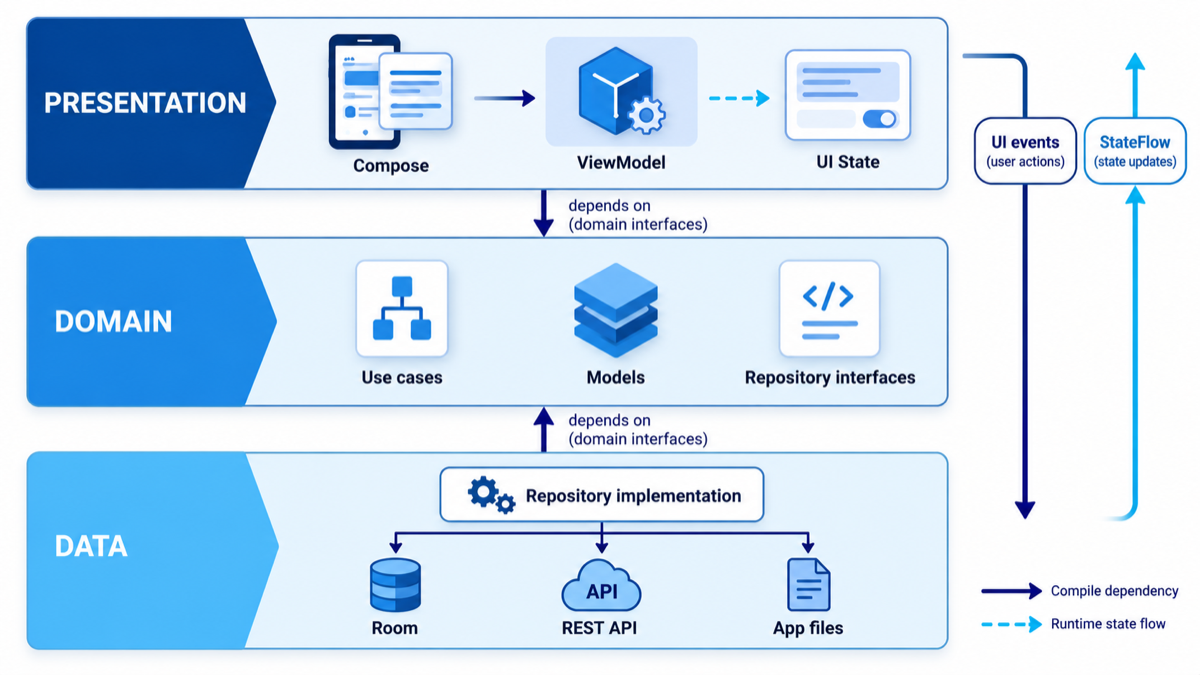
\includegraphics[width=\linewidth]{figures/Kiến trúc ba lớp.png}
\end{column}
\end{columns}
\end{frame}

% ------------------------------------------------------------
\subsection{Cấu trúc mô-đun}
% ------------------------------------------------------------
\begin{frame}{Cấu trúc mô-đun}
\begin{columns}[T]
\begin{column}{0.52\textwidth}
\footnotesize
\begin{itemize}\setlength{\itemsep}{3pt}
\item \textbf{:app} lắp ghép: MainActivity, shell, root routing, Hilt wiring
\item \textbf{Feature} sở hữu màn hình: mỗi phân hệ một module feature (video, music, news, games, onboarding, account\ldots)
\item \textbf{Domain, data và core} được quản lý riêng: domain một module Kotlin thuần; data theo phân hệ; core theo vai trò (design system, session, media, database, datastore, network)
\item Kiểm tra phụ thuộc \textbf{tự động} bằng tác vụ \texttt{verifyArchitecture}
\end{itemize}
\end{column}
\begin{column}{0.42\textwidth}
\centering
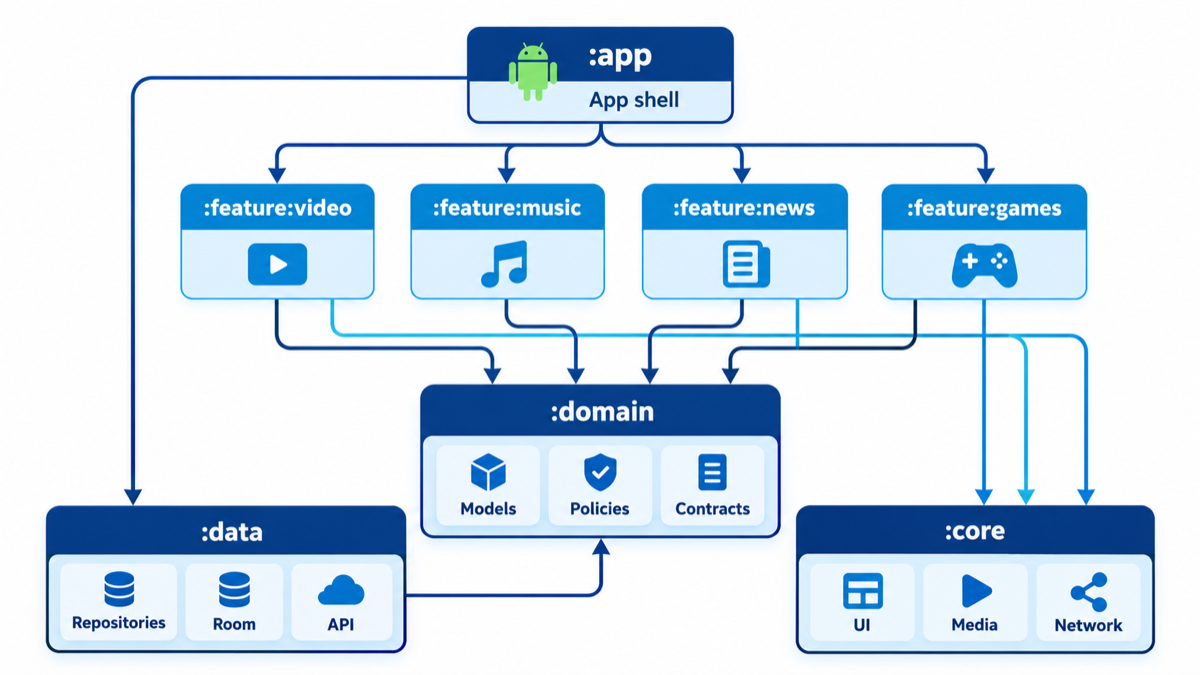
\includegraphics[width=\linewidth]{figures/Cấu trúc mô-đun.png}
\end{column}
\end{columns}
\end{frame}

% ------------------------------------------------------------
\subsection{Điều hướng do app quản lý}
% ------------------------------------------------------------
\begin{frame}{Điều hướng do app quản lý}
\centering
{\small App chọn luồng khởi động và quản lý Back. Feature cung cấp route và graph của mình.}\vspace{2.5mm}

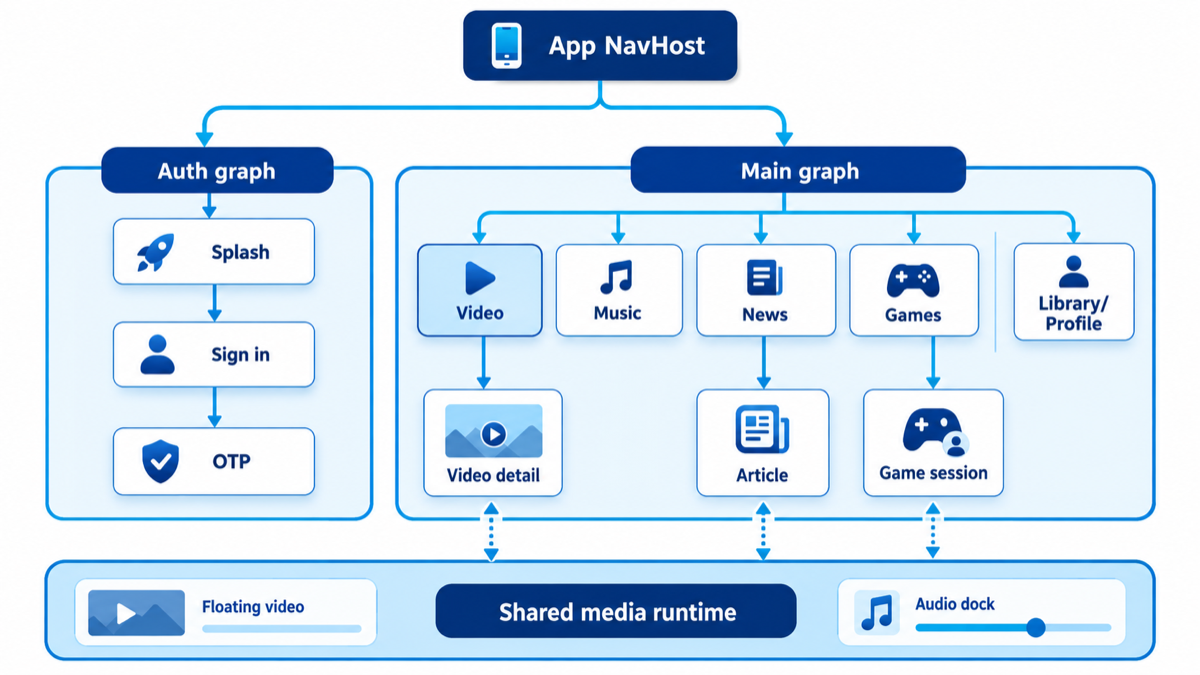
\includegraphics[width=10.5cm]{figures/Điều hướng do app quản lý.png}
\end{frame}

% ------------------------------------------------------------
\subsection{Nội dung và dữ liệu lấy từ đâu?}
% ------------------------------------------------------------
\begin{frame}{Nội dung và dữ liệu lấy từ đâu?}
\small
\centering
\begin{tabular}{@{}p{3.3cm}p{5.3cm}p{5.6cm}@{}}
\toprule
\textbf{Loại dữ liệu} & \textbf{Nguồn dự kiến} & \textbf{Ứng dụng nhận được gì?} \\
\midrule
Video và nhạc & Tệp nhóm tự tạo hoặc được phép dùng & Nhóm upload kho media, API trả danh mục \\
Bài đọc và nghe tin TTS & Bài nhóm biên soạn hoặc được phép lưu toàn văn & Nội dung để đọc trong app và tạo tiếng nói \\
Tin từ nguồn ngoài & Dự kiến RSS VnExpress, có ghi nguồn & Tiêu đề, tóm tắt và link về bài gốc \\
Game và dữ liệu tài khoản & Luật game trong app, cấu hình và API của nhóm & Quiz, nhiệm vụ, playlist và dữ liệu cá nhân \\
\bottomrule
\end{tabular}

\vspace{0.3cm}
{\footnotesize\color{TextGray} Kho nội dung mẫu trong phạm vi môn học: 50 video, 50 bài hát, 50 bài báo~--~tự dựng hoặc được phép dùng.}
\end{frame}

% ------------------------------------------------------------
\subsection{Upload và phát nội dung}
% ------------------------------------------------------------
\begin{frame}{Upload và phát nội dung}
\begin{center}
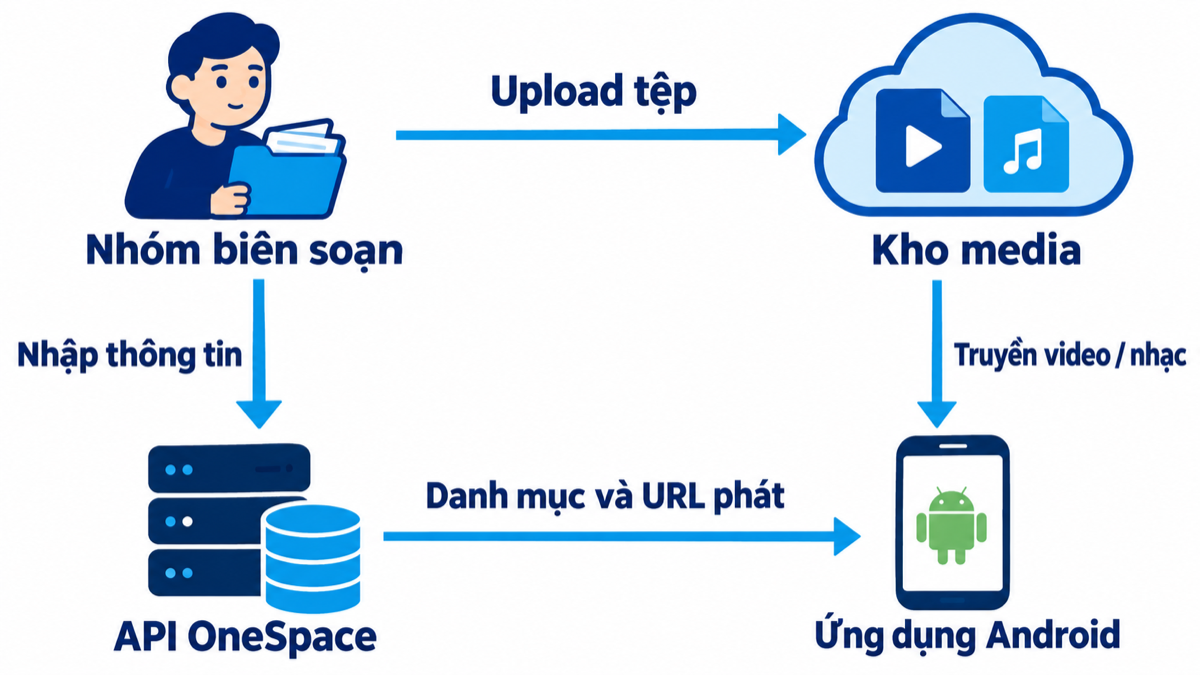
\includegraphics[width=8.2cm]{figures/Upload và phát nội dung.png}
\end{center}
\vspace{1.5mm}
\small
\begin{itemize}\setlength{\itemsep}{3pt}
\item App gọi API lấy danh mục (tiêu đề, mô tả, URL); media stream thẳng từ kho media qua bộ phát Media3
\item Thay nguồn $=$ thay URL: player, UI và logic phát không đổi
\item Quiz, nhiệm vụ, câu hỏi soạn sẵn đi kèm nội dung khi đăng
\end{itemize}
\end{frame}

% ------------------------------------------------------------
\subsection{Dữ liệu được lưu ở đâu?}
% ------------------------------------------------------------
\begin{frame}{Dữ liệu được lưu ở đâu?}
\small
\centering
\begin{tabular}{@{}p{3.0cm}p{5.4cm}p{5.6cm}@{}}
\toprule
\textbf{Nơi lưu} & \textbf{Dữ liệu chính} & \textbf{Ý nghĩa} \\
\midrule
Room trên điện thoại & Danh mục đã lấy, bookmark, tiến độ & Đọc lại dữ liệu đã lưu khi mất mạng \\
DataStore & Thiết lập nhỏ của thiết bị & Ghi nhớ cấu hình giao diện và phát \\
Tệp riêng của ứng dụng & TTS và MP3 đã tạo hoặc tải hoàn tất & Lưu tệp âm thanh, tách khỏi cache tạm \\
Server và kho media & Tài khoản, playlist đồng bộ, điểm và tệp gốc & Quản lý dữ liệu chung và quyền truy cập \\
\bottomrule
\end{tabular}

\vspace{0.3cm}
{\footnotesize\color{TextGray} Nguyên tắc offline-first: mọi dữ liệu đã xem có bản lưu cục bộ; đồng bộ lại khi có mạng.}
\end{frame}

% ------------------------------------------------------------
\subsection{Mô hình dữ liệu và API}
% ------------------------------------------------------------
\begin{frame}{Mô hình dữ liệu (physical) --- ERD Room schema v5}
\begin{center}
\begin{tikzpicture}[font=\tiny]
  % ===== video_progress =====
  \draw[draw=BKTemplate, thick] (0,0) rectangle (4.0,-1.45);
  \fill[BKTemplate] (0,0) rectangle (4.0,-0.3);
  \node[text=white, font=\tiny\bfseries] at (2.0,-0.15) {video\_progress};
  \node[anchor=north west, align=left, inner sep=3pt] at (0.03,-0.33) {\underline{videoId}~PK (FK logic)\\title\\positionMs (vị trí xem)\\updatedAt};
  % ===== watchlist =====
  \draw[draw=BKTemplate, thick] (4.3,0) rectangle (8.3,-1.3);
  \fill[BKTemplate] (4.3,0) rectangle (8.3,-0.3);
  \node[text=white, font=\tiny\bfseries] at (6.3,-0.15) {watchlist};
  \node[anchor=north west, align=left, inner sep=3pt] at (4.33,-0.33) {\underline{videoId}~PK (FK logic)\\title\\savedAt};
  % ===== point_entries (nhóm: gamification) =====
  \draw[draw=GreenOK!65!black, thick] (8.6,0) rectangle (12.6,-1.45);
  \fill[GreenOK!65!black] (8.6,0) rectangle (12.6,-0.3);
  \node[text=white, font=\tiny\bfseries] at (10.6,-0.15) {point\_entries};
  \node[anchor=north west, align=left, inner sep=3pt] at (8.63,-0.33) {\underline{id}~PK (tự tăng)\\source\\amount\\timestamp};
  % ===== daily_missions (nhóm: gamification) =====
  \draw[draw=GreenOK!65!black, thick] (0,-1.65) rectangle (4.0,-3.6);
  \fill[GreenOK!65!black] (0,-1.65) rectangle (4.0,-1.95);
  \node[text=white, font=\tiny\bfseries] at (2.0,-1.8) {daily\_missions};
  \node[anchor=north west, align=left, inner sep=3pt] at (0.03,-1.98) {\underline{id}~PK\\title\\targetType $\cdot$ target\\progress $\cdot$ completed\\date (mỗi ngày)};
  % ===== extracted_audio (nhóm: thư viện âm thanh) =====
  \draw[draw=BKLight, thick] (4.3,-1.65) rectangle (8.3,-3.35);
  \fill[BKLight] (4.3,-1.65) rectangle (8.3,-1.95);
  \node[text=white, font=\tiny\bfseries] at (6.3,-1.8) {extracted\_audio};
  \node[anchor=north west, align=left, inner sep=3pt] at (4.33,-1.98) {\underline{videoId}~PK (FK logic)\\title $\cdot$ creator\\url $\cdot$ duration\\extractedAt};
  % ===== downloaded_content (nhóm: thư viện offline) =====
  \draw[draw=BKLight, thick] (8.6,-1.65) rectangle (12.6,-3.35);
  \fill[BKLight] (8.6,-1.65) rectangle (12.6,-1.95);
  \node[text=white, font=\tiny\bfseries] at (10.6,-1.8) {downloaded\_content};
  \node[anchor=north west, align=left, inner sep=3pt] at (8.63,-1.98) {\underline{contentId}~PK (FK logic)\\type (video / nhạc / tin)\\title $\cdot$ subtitle\\downloadedAt};
  % ===== DataStore + tệp =====
  \node[draw=BKLight, thick, rounded corners=3pt, fill=BKLight!10, align=left, inner sep=4pt, anchor=north west, text width=11.2cm, font=\tiny] at (0.35,-3.95) {\textbf{DataStore (preferences):} phiên đăng nhập $\cdot$ cài đặt $\cdot$ bài tin đã lưu $\cdot$ playlist (JSON) $\cdot$ trạng thái game (streak, pet, shop)\\[1pt]\textbf{Tệp riêng của ứng dụng:} MP3 trích từ video, TTS đã tạo};
  \node[font=\tiny, text=TextGray, align=center, text width=12.4cm] at (6.3,-5.15) {videoId / contentId là khóa ngoại \textbf{logic} (tham chiếu mềm) tới danh mục; không có FK vật lý --- ràng buộc do repository trong app đảm bảo.\\ Màu tiêu đề: xanh đậm = tương tác nội dung $\cdot$ xanh lam = thư viện offline (tải về / trích xuất) $\cdot$ xanh lá = gamification.};
\end{tikzpicture}
\end{center}
\end{frame}

% ------------------------------------------------------------
\begin{frame}{Mô hình dữ liệu backend (thiết kế giai đoạn remote)}
\begin{center}\tiny
\setlength{\tabcolsep}{3pt}
\begin{tabular}{@{}p{2.4cm}p{2.6cm}p{4.4cm}p{3.5cm}@{}}
\toprule
\textbf{Entity} & \textbf{Khóa chính} & \textbf{Trường chính} & \textbf{Quan hệ} \\
\midrule
users & id & phone, name, avatar, created\_at & 1--n playlists, point\_entries, missions, progress \\
content\_items & id & type (video / nhạc / tin), title, url, duration, published\_at & 1--n playlist\_items, progress \\
playlists & id & user\_id, name, updated\_at & thuộc users; 1--n playlist\_items \\
playlist\_items & (playlist\_id, item\_id) & position & thuộc playlists; trỏ content\_items \\
point\_entries & id & user\_id, source, amount, created\_at & thuộc users (ledger điểm) \\
daily\_missions & id & user\_id, title, target, progress, date & thuộc users \\
progress & (user\_id, item\_id) & position\_ms, updated\_at & thuộc users + content\_items \\
\bottomrule
\end{tabular}
\end{center}
\vspace{1.2mm}
{\tiny\color{TextGray} Thiết kế cho giai đoạn remote (ADR-17)~--~chưa hiện thực; khớp endpoint ở slide sau. Bản đang chạy trên máy là ERD Room ở slide trước (6 bảng cục bộ).}
\end{frame}

% ------------------------------------------------------------
\begin{frame}{Thiết kế API (giai đoạn remote)}
{\tiny\color{TextGray} REST + JSON, HTTPS TLS 1.2 trở lên, token định danh (SEC-03). Thiết kế cho giai đoạn remote~--~app hiện dùng mock repository cùng interface nên thay thế không đụng UI.}
\vspace{1.2mm}
\begin{center}\tiny
\begin{tabular}{@{}llp{4.4cm}p{5.0cm}@{}}
\toprule
\textbf{Method} & \textbf{Endpoint} & \textbf{Ý nghĩa} & \textbf{Trả về chính} \\
\midrule
GET & /catalog/videos & Danh mục video & id, title, creator, duration, url, thumbnail \\
GET & /catalog/tracks & Danh mục nhạc & id, title, artist, album, duration, url \\
\midrule
GET & /news/articles & Danh sách tin & id, title, summary, source, publishedAt \\
GET & /news/articles/\{id\} & Chi tiết bài & toàn văn, quiz, bài liên quan \\
\midrule
POST & /auth/otp & Gửi OTP SMS & thời hạn 5 phút (SEC-01) \\
POST & /auth/verify & Đổi OTP lấy token & token, hồ sơ người dùng \\
\midrule
GET & /me/playlists & Playlist của tôi & id, tên, danh sách mục \\
POST & /me/playlists & Tạo / sửa playlist & playlist đã lưu \\
POST & /me/points & Ghi điểm, nhiệm vụ & số dư, nhiệm vụ hôm nay \\
\bottomrule
\end{tabular}
\end{center}
\vspace{0.5mm}
{\tiny\color{TextGray} Phân trang: \texttt{?page=\&limit=}; đồng bộ xung đột theo ID + version.}
\end{frame}

% ------------------------------------------------------------
\begin{frame}{API: mẫu phản hồi và xử lý mã lỗi}
\begin{columns}[T]
\begin{column}{0.42\textwidth}
{\small\textbf{Mẫu phản hồi}}\\[0.8mm]
{\tiny\ttfamily
GET /catalog/videos?page=1\\[0.5mm]
\{"items": [\\
~~"id": "v01",\\
~~"title": "Giới thiệu OneSpace",\\
~~"creator": "Nhóm OneSpace",\\
~~"duration": 213,\\
~~"url": "https://\ldots/oceans.mp4",\\
~~"thumbnail": "https://\ldots/v01.jpg"\\
], "page": 1, "hasMore": true\}}
\end{column}
\begin{column}{0.56\textwidth}
{\small\textbf{Mã lỗi chuẩn HTTP}}\\[0.8mm]
{\tiny
\begin{tabular}{@{}llp{4.4cm}@{}}
\toprule
\textbf{Mã} & \textbf{Ý nghĩa} & \textbf{App xử lý} \\
\midrule
400 & Sai tham số & Thông báo, giữ dữ liệu cũ \\
401 & Token hết hạn & Yêu cầu đăng nhập lại \\
403 & Không có quyền & Ẩn hành động cần quyền \\
404 & Không có nội dung & EmptyState + gợi ý thay thế \\
409 & Xung đột phiên bản & Giữ bản mới hơn, sync lại \\
429 & Quá nhiều request & Chờ rồi tự thử lại \\
5xx & Lỗi server & ``Không tải được'' + Thử lại \\
\bottomrule
\end{tabular}}
\vspace{1.5mm}

{\tiny\color{TextGray} Lỗi player và lỗi request hiện qua ErrorState dùng chung; connectivity chỉ là tín hiệu gợi ý~--~kết quả thao tác do lỗi thật quyết định.}
\end{column}
\end{columns}
\end{frame}

% ------------------------------------------------------------
\subsection{Luồng chính: sequence diagram}
% ------------------------------------------------------------
\begin{frame}{Sequence diagram: xung đột âm thanh (C1)}
\begin{center}
\begin{tikzpicture}[
  font=\tiny,
  ll/.style={draw=BKTemplate, thick, rounded corners=2pt, fill=BKTemplate!10, minimum width=2.15cm, minimum height=0.5cm, align=center},
  msg/.style={-{Latex[length=1.5mm]}, thick},
  ret/.style={-{Latex[length=1.5mm]}, thick, dashed},
  note/.style={draw=OrangeWarn, fill=OrangeWarn!12, rounded corners=2pt, inner sep=2.5pt, align=center}]
  \node[ll] (u)  at (1.1,6.45) {\bfseries Người dùng};
  \node[ll] (ui) at (3.9,6.45) {Màn Nhạc (UI)};
  \node[ll] (sp) at (6.8,6.45) {Session\\Coordinator};
  \node[ll] (mc) at (9.7,6.45) {Media\\Coordinator};
  \node[ll] (pl) at (12.55,6.45) {2 Player\\(nhạc $\cdot$ video)};
  \foreach \n in {u,ui,sp,mc,pl} \draw[dashed, TextGray!60] (\n.south) -- ++(0,-4.6);
  % Thanh kích hoạt (execution specification)
  \foreach \bx/\ya/\yb in {3.9/5.4/5.9, 6.8/1.75/5.4, 9.7/2.45/3.5, 12.55/2.45/3.0}{
    \draw[fill=white, draw=black!60, thick] (\bx-0.07,\ya) rectangle (\bx+0.07,\yb);}
  \draw[msg] (1.1,5.9) -- (3.9,5.9) node[midway, above]{1. Mở bài nhạc (video đang phát)};
  \draw[msg] (3.9,5.4) -- (6.8,5.4) node[midway, above]{2. Xin quyết định luồng tiếng};
  \node[note] at (8.6,5.0) {chưa có quy tắc đã lưu};
  \draw[dashed, TextGray] (6.8,5.28) -- (7.6,5.03);
  \draw[ret] (6.8,4.5) -- (1.1,4.5) node[midway, above]{3. Popup 2 lựa chọn + ô tick (F-COM-14)};
  \draw[msg] (1.1,4.0) -- (6.8,4.0) node[midway, above]{4. Chọn ``Tắt tiếng video''};
  \draw[msg] (6.8,3.5) -- (9.7,3.5) node[midway, above]{5. Áp dụng chính sách};
  \draw[msg] (9.7,3.0) -- (12.55,3.0) node[midway, above, align=center]{6. Video: còn hình,\\tắt tiếng};
  \draw[msg] (9.7,2.45) -- (12.55,2.45) node[midway, above, align=center]{7. Nhạc: phát tiếp,\\nguồn tiếng chính};
  \node[note] at (9.35,1.8) {tick ``Không hỏi lại'' $\Rightarrow$ lần sau áp dụng im lặng};
  \draw[dashed, TextGray] (6.8,2.1) -- (7.4,1.86);
\end{tikzpicture}
\end{center}
\vfill
{\tiny\color{TextGray} Lựa chọn còn lại: ``Dừng video''~--~video dừng và lưu vào Xem sau đúng vị trí.}
\end{frame}

% ------------------------------------------------------------
\begin{frame}{Sequence diagram: khởi động và khôi phục phiên}
\begin{center}
\begin{tikzpicture}[
  font=\tiny,
  ll/.style={draw=BKTemplate, thick, rounded corners=2pt, fill=BKTemplate!10, minimum width=2.15cm, minimum height=0.5cm, align=center},
  msg/.style={-{Latex[length=1.5mm]}, thick},
  ret/.style={-{Latex[length=1.5mm]}, thick, dashed},
  note/.style={draw=OrangeWarn, fill=OrangeWarn!12, rounded corners=2pt, inner sep=2.5pt, align=center}]
  \node[ll] (u)    at (1.1,6.45) {\bfseries Người dùng};
  \node[ll] (os)   at (3.9,6.45) {Hệ điều hành};
  \node[ll] (app)  at (6.8,6.45) {App\\(Splash $\rightarrow$ Main)};
  \node[ll] (st)   at (9.7,6.45) {DataStore\\+ Room};
  \node[ll] (ss)   at (12.55,6.45) {Session\\Coordinator};
  \foreach \n in {u,os,app,st,ss} \draw[dashed, TextGray!60] (\n.south) -- ++(0,-4.6);
  % Thanh kích hoạt
  \foreach \bx/\ya/\yb in {6.8/3.9/5.4, 9.7/4.4/4.9, 12.55/3.1/3.9}{
    \draw[fill=white, draw=black!60, thick] (\bx-0.07,\ya) rectangle (\bx+0.07,\yb);}
  \draw[msg] (1.1,5.9) -- (3.9,5.9) node[midway, above]{1. Mở lại app (sau khi tiến trình bị hủy)};
  \draw[msg] (3.9,5.4) -- (6.8,5.4) node[midway, above]{2. Khởi động process + MainActivity (splash giữ theo state)};
  \draw[msg] (6.8,4.9) -- (9.7,4.9) node[midway, above]{3. Đọc onespace\_session, hydrate playlist};
  \draw[ret] (9.7,4.4) -- (6.8,4.4) node[midway, above]{4. tab cuối, bài cuối, playlists, điểm/streak};
  \draw[msg] (6.8,3.9) -- (12.55,3.9) node[midway, above]{5. restoreColdStartSession(): mở tab cuối; đặt bài cuối ở 0:00};
  \node[note] at (10.85,3.02) {nhạc không tự phát\\--~bấm play trên dock};
  \draw[dashed, TextGray] (12.55,3.35) -- (12.1,3.08);
  \node[note, align=center] at (7.3,1.95) {Mở lại video dở: checkpoint Room 3 giây $\rightarrow$ seek đúng vị trí};
  \draw[dashed, TextGray] (9.7,2.2) -- (9.55,2.02);
\end{tikzpicture}
\end{center}
\vfill
{\tiny\color{TextGray} Đã đối chiếu code: tab cuối + bài cuối (trạng thái dừng) + playlist + vị trí video khi mở lại video + điểm/streak/pet giữ nguyên. Vị trí đọc tin và ván game qua process death, tự phát lại nhạc: hạng mục sau~--~xem bảng kiểm chứng kiến trúc trong báo cáo.}
\end{frame}

% ------------------------------------------------------------
\subsection{Phối hợp video, nhạc và các màn hình}
% ------------------------------------------------------------
\begin{frame}{Phối hợp video, nhạc và các màn hình}
\small
\begin{enumerate}\setlength{\itemsep}{5pt}
\item \textbf{Dùng chung bộ phát}~--~Một bộ phát video và một bộ phát audio phục vụ toàn ứng dụng (Media3); bốn phân hệ không tự dựng player riêng
\item \textbf{Chọn âm thanh chính}~--~Video có tiếng và nhạc cùng phát: hỏi người dùng giữ nguồn nào (popup C1/C2 kèm ô tick ``Không hỏi lại''); một thời điểm chỉ một nguồn tiếng chính
\item \textbf{Hiệu ứng game lớp riêng (F-GAME-13)}~--~SFX qua SoundPool sonification, tự giảm còn 25\% khi nhạc/video/TTS đang phát, mức âm chỉnh trong Cài đặt; không xin audio focus
\item \textbf{Giữ phiên khi chuyển màn hình}~--~Video nổi và audio dock tiếp tục điều khiển cùng phiên phát; quay lại đúng vị trí (lệch $\leq$ 2 giây), kể cả khi hệ điều hành đã hủy app
\end{enumerate}
\vspace{1mm}
\begin{exampleblock}{Kết quả}
Người dùng nghe nhạc khi đọc tin, xem video nổi khi lướt feed, chơi game với nhạc nền~--~một trải nghiệm liền mạch thay vì bốn ứng dụng riêng.
\end{exampleblock}
\end{frame}

% ------------------------------------------------------------
\begin{frame}{Sequence diagram: xem video và chuyển phân hệ (X1)}
\begin{center}
\begin{tikzpicture}[
  font=\tiny,
  ll/.style={draw=BKTemplate, thick, rounded corners=2pt, fill=BKTemplate!10, minimum width=2.15cm, minimum height=0.5cm, align=center},
  msg/.style={-{Latex[length=1.5mm]}, thick},
  ret/.style={-{Latex[length=1.5mm]}, thick, dashed},
  note/.style={draw=OrangeWarn, fill=OrangeWarn!12, rounded corners=2pt, inner sep=2.5pt, align=center}]
  \node[ll] (u)  at (1.1,6.45) {\bfseries Người dùng};
  \node[ll] (ui) at (3.9,6.45) {Màn Video (UI)};
  \node[ll] (sc) at (6.8,6.45) {Session\\Coordinator};
  \node[ll] (pv) at (9.7,6.45) {Video engine\\(Media3)};
  \node[ll] (sh) at (12.55,6.45) {Shell\\(cửa sổ nổi)};
  \foreach \n in {u,ui,sc,pv,sh} \draw[dashed, TextGray!60] (\n.south) -- ++(0,-4.6);
  % Thanh kích hoạt
  \foreach \bx/\ya/\yb in {3.9/4.35/5.9, 6.8/4.85/5.4, 9.7/4.35/4.95, 12.55/2.5/3.95}{
    \draw[fill=white, draw=black!60, thick] (\bx-0.07,\ya) rectangle (\bx+0.07,\yb);}
  \draw[msg] (1.1,5.9) -- (3.9,5.9) node[midway, above]{1. Chạm video trong feed};
  \draw[msg] (3.9,5.4) -- (6.8,5.4) node[midway, above, align=center]{2. playVideo(id): đọc vị trí đã lưu; nhạc đang phát $\rightarrow$ popup C2 (X0)};
  \draw[msg] (6.8,4.9) -- (9.7,4.9) node[midway, above]{3. Mở stream tại resumeFrom};
  \draw[ret] (9.7,4.4) -- (3.9,4.4) node[midway, above]{4. Phát tiếp tại vị trí đã lưu ($\leq$ 2 giây)};
  \draw[msg] (1.1,3.9) -- (12.55,3.9) node[midway, above]{5. Chọn tab khác (ví dụ Tin tức)};
  \node[note] at (10.8,3.05) {videoDocked = true\\cửa sổ nổi hiện, vẫn phát};
  \draw[dashed, TextGray] (12.55,3.5) -- (12.1,3.1);
  \draw[msg] (12.55,2.5) -- (3.9,2.5) node[midway, above]{6. Chạm ``Mở rộng'': mở lại player, cùng engine, đúng vị trí};
  \node[note] at (9.2,1.75) {Đóng cửa sổ nổi: dừng + lưu vị trí + thêm Xem sau};
  \draw[dashed, TextGray] (12.55,2.2) -- (10.85,1.8);
\end{tikzpicture}
\end{center}
\vfill
{\tiny\color{TextGray} Kịch bản theo code thật: OneSpaceApp (videoDocked), SessionPlayers (FloatingVideo), MediaPlaybackCoordinator (cùng engine). Tab đích là Home: phát trong card feed, không cửa sổ nổi.}
\end{frame}

% ------------------------------------------------------------
\subsection{Nghe tin TTS và tạo MP3}
% ------------------------------------------------------------
\begin{frame}{Nghe tin TTS và tạo MP3}
\begin{columns}[T]
\begin{column}{0.54\textwidth}
\footnotesize
\begin{itemize}\setlength{\itemsep}{3pt}
\item \textbf{TTS đọc bài báo:} nút ``Nghe tin'' trong trình đọc $\rightarrow$ TTS on-device đọc bài; nhạc đang phát tự nhường (C13)
\item \textbf{Tạo file MP3 thật:} bản audio của bài (TTS) và bản trích từ video (F-VID-10) được ghi thành tệp mp3 trong tệp riêng của ứng dụng
\item Tệp phát lại như một bài nhạc thường: điều khiển bằng dock mini, đưa vào hàng đợi, xoá được
\item Engine TTS là \textbf{module thay được}: on-device (miễn phí, chất lượng vừa) hoặc API cloud (chất lượng, phí theo ký tự)~--~đổi hướng không đụng UI
\end{itemize}
\end{column}
\begin{column}{0.40\textwidth}
\centering
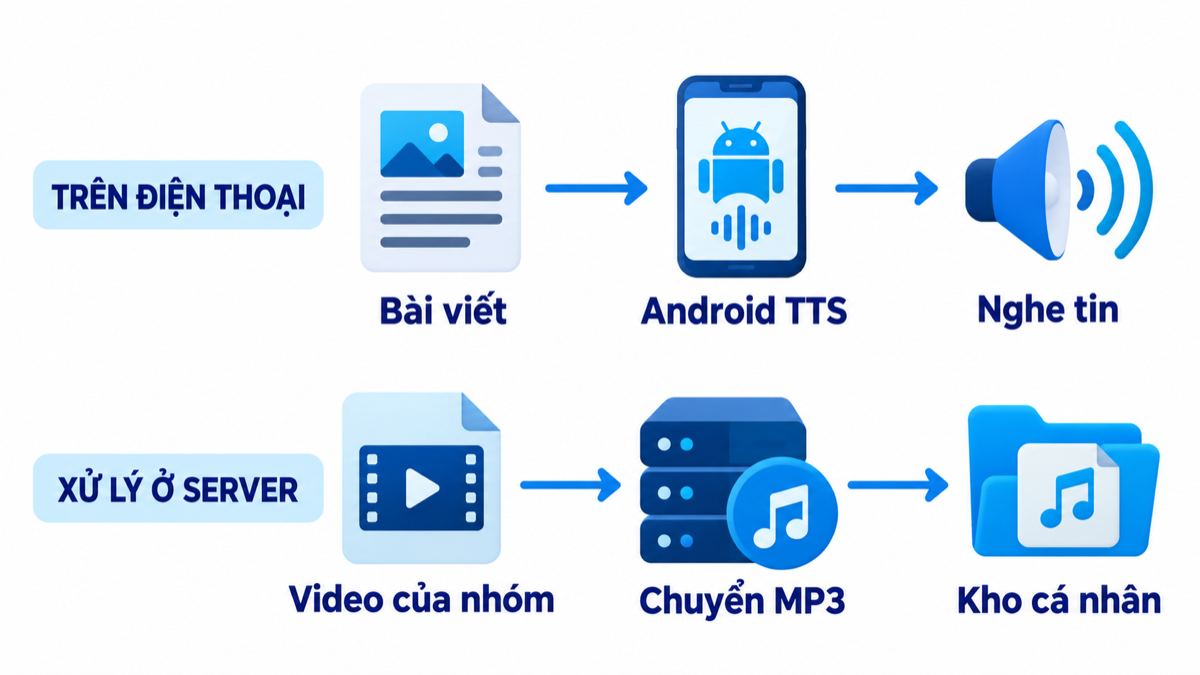
\includegraphics[width=\linewidth]{figures/Nghe tin TTS và tạo MP3.png}
\end{column}
\end{columns}
\end{frame}

% ------------------------------------------------------------
\subsection{Ma trận truy vết}
% ------------------------------------------------------------
\begin{frame}{Ma trận truy vết (requirement $\rightarrow$ kiến trúc)}
\begin{center}\tiny
\setlength{\tabcolsep}{3pt}
\begin{tabular}{@{}p{4.0cm}p{3.0cm}p{2.5cm}p{3.8cm}@{}}
\toprule
\textbf{Yêu cầu (kèm user story)} & \textbf{Use case} & \textbf{Màn hình} & \textbf{Thành phần kiến trúc} \\
\midrule
F-VID-01 · US-VID-01 & Xem video (UC-02) & Mockup F-VID-01 & feature/video + core/media \\
F-VID-08 · US-VID-02, US-CROSS-03 & Tiếp tục xem khi chuyển phân hệ (X1) & Mockup F-VID-08 & app (shell) + core/session \\
F-MUS-02 · US-MUS-02, US-CROSS-01 & Nghe nhạc (UC-03) & Mockup F-MUS-02 & core/session + core/media \\
F-COM-14 · US-MUS-03, US-CROSS-02 & Xử lý xung đột âm thanh (X0) & Mockup F-COM-14 & domain (SessionPolicy) + app \\
F-NEWS-05 · US-NEWS-04, US-CROSS-08 & Nghe tin TTS (X4) & Mockup F-NEWS-05 & feature/news + core/media (TTS) \\
F-GAME-02 · US-GAME-02 & Chơi minigame (UC-05) & Mockup F-GAME-02 & feature/games + core/media \\
F-COM-01 · US-COM-01 & Quản lý danh tính (UC-11) & Mockup F-COM-01 & feature/auth + core/datastore \\
\bottomrule
\end{tabular}
\end{center}
\vspace{1.5mm}
{\tiny\color{TextGray} Chuỗi đầy đủ: yêu cầu $\rightarrow$ use case (sơ đồ tổng quan) $\rightarrow$ user story kèm AC $\rightarrow$ màn hình (mock up ảnh thật) $\rightarrow$ module kiến trúc. Tổng: \textbf{76} yêu cầu $\rightarrow$ \textbf{45} story (100\% có AC) $\rightarrow$ \textbf{74} mã có ảnh chụp $\rightarrow$ \textbf{23} mô-đun Gradle.}
\end{frame}


% ============================================================
% THANK YOU
% ============================================================
\setbeamertemplate{footline}{}
\begin{frame}
    \centering
    \vspace{0.3cm}
    \textbf{\Huge{Cảm ơn thầy và các bạn}}\\
    \vspace{0.55cm}

    {\small Phạm Khánh Duy (2310510) \quad·\quad Nguyễn Trần Yến Nhi (2312506) \quad·\quad Tăng Hồng Ái (2310167)}\\
    \vspace{0.25cm}
    {\small CO3043 --- Phát triển Ứng dụng trên Thiết bị Di động \quad·\quad Bài tập lớn}\\
    \vspace{0.15cm}
    {\scriptsize \color{TextGray} Khoa Khoa học và Kỹ thuật Máy tính\\[0.5mm]
    GVHD: TS.\ Phan Trần Minh Khuê}
\end{frame}

\end{document}
